\documentclass[a4paper,12pt]{article}
\documentclass[a4paper,12pt]{article}
\usepackage[german]{babel}
\usepackage{amsfonts,amsmath,amssymb,bbm,wasysym,mathrsfs}
\usepackage{enumerate}
\usepackage{makeidx}
\usepackage[german,norefeq,norefpage]{nomencl}
\makeindex
\usepackage[style=long,border=none,header=plain,cols=3]{glossary}
\makeglossary
\usepackage{graphicx,color}
\usepackage[nottoc]{tocbibind}
\usepackage[only, lightning]{stmaryrd}
%\usepackage[squaren]{SIunits}
\makeatletter
\providecommand{\LyX}{L\kern-.1667em\lower.25em\hbox{Y}\kern-.125emX\@}
\providecommand{\fertig}{$\blacksquare$}
\usepackage{geometry}
\usepackage{multicol}
\usepackage{fancyhdr}
\pagestyle{fancy}
\hoffset=5 pt
\headheight =28pt
\headsep=20pt
\footskip = 40pt
\textheight =650pt
\fancyfoot{\empty}
\fancyfoot[L]{\today}
\fancyfoot[R]{\thepage}
\fancyhead{\empty}
\lhead{
\begin{picture}(0,0)
\put(-80,-340){\line(10,0){10}}
\end{picture}
}
\rhead{\hfill {\bf \leftmark}\newline\rightmark}
\usepackage{tocloft}
\addtolength{\cftsecindent}{-1em}
\addtolength{\cftsecnumwidth}{1em}
\usepackage{xy}
	\input xy
	\xyoption{all}
\usepackage{theorem}
	\theorembodyfont{\upshape}
	\newtheorem{definition}{Definition:}[section]
	\newtheorem{satz}[definition]{Satz:}
	\newtheorem{kor}[definition]{Korollar:}
	\newtheorem{prop}[definition]{Proposition}
	\newtheorem{lemma}[definition]{Lemma:}
	\newtheorem{bem}[definition]{Bemerkung:}
	\newtheorem{beispiel}[definition]{Beispiel:}
	\newtheorem{beob}[definition]{Beobachtung:}

	\renewcommand{\thesection}{\Roman{section}}
	\renewcommand{\thesubsection}{\arabic{subsection}}
	
	\newcommand{\beweis}[1]{\begin{description}\item[\ul{Beweis:}] #1 \hfill\fertig\end{description}}
	
	\newcommand{\N}{\mathbb N} \newcommand{\Z}{\mathbb Z} \newcommand{\R}{\mathbb R}
	\newcommand{\Q}{\mathbb Q}\newcommand{\C}{\mathbb C}
	\newcommand{\surj}{\twoheadrightarrow}
	\newcommand{\inj}{\rightarrowtail}
	\newcommand{\ra}{\rightarrow}
	\newcommand{\ramit}[1]{\stackrel{#1}{\longrightarrow}}
	\newcommand{\impl}{\Rightarrow}\newcommand{\lpmi}{\Leftarrow}
	\newcommand{\implmit}[1]{\stackrel{#1}{\Longrightarrow}}
	\newcommand{\lpmimit}[1]{\stackrel{#1}{\Longleftarrow}}
	\newcommand{\gleichmit}[1]{\stackrel{#1}{=}}
	\newcommand{\seq}{\subseteq }
	\newcommand{\ul}{\underline }
	\newcommand{\inv}[1]{#1^{-1}}
	\newcommand{\eq}{\Leftrightarrow}
	\newcommand{\eqmit}[1]{\stackrel{#1}{\eq}}
	\newcommand{\eps}{\varepsilon}
	\renewcommand{\ker}[1]{{\bf ker} #1 }
	\newcommand{\norm}[1]{\|{ #1 }\|}
	\newcommand{\ol}[1]{\overline{#1}}
	\newcommand{\durch}[1]{\frac{1}{#1}}
	\newcommand{\leer}{\emptyset}
	\newcommand{\et}{\wedge}
	\newcommand{\vel}{\vee}
	\newcommand{\ovec}{\mathfrak o}
	\newcommand{\innprod}[2]{<\hspace*{-0.15cm} #1|#2\hspace*{-0.15cm} >}
	\newcommand{\wid}{\mbox{\large\mbox{$\lightning$}}}
	\newcommand{\todo}[1]{\mbox{\textcolor{red}{$\clubsuit$} #1 \textcolor{red}{$\spadesuit$}}}
	\newcommand{\pr}{\mbox{pr}}
	\newcommand{\blitzmit}[2]{\stackrel{\stackrel{#2}{\lightning}}{#1}}

\setcounter{section}{-1}
\title{Grundbegriffe der Topologie\vspace*{-0.3cm}\\{\scriptsize nach einer Vorlesung von Michael Grosser}\\WS 0405}
\author{Martin Heuschober}
\date~
	\newcommand{\umgbas}[2]{{\mathcal #1}_{#2}}
	\newcommand{\umg}[2]{{\mathscr #1}_{#2}}
	\newcommand{\T}{\mathcal T}
	\newcommand{\B}{\mathcal B}
	\newcommand{\Sb}{\mathcal S}
	\newcommand{\A}{\mathcal A}
	\newcommand{\closure}{\complement}
	\newcommand{\cl}[1]{\closure (#1 )}
	\newcommand{\inn}[1]{#1^\circ}
	\newcommand{\ext}[1]{\mbox{ext}(#1)}
	\newcommand{\bd}[1]{\partial #1}
	\newcommand{\isol}[1]{\mbox{Isol}(#1 )}
	\newcommand{\Kappa}{\mbox{\large\mbox{$\varkappa$}}}
	\newcommand{\trax}{\mbox{\sf T}}

	\renewcommand{\theequation}{$\bigstar _{\arabic{equation}}$}
\begin{document}
%
\nomenclature{$\N$}{die Menge der nat{\"u}rlichen Zahlen; $\{ 1, 2, 3, \dots\}$}%
\nomenclature{$\Z$}{die Menge der ganzen Zahlen; $\{ 0, \pm 1,\pm 2,\pm 3, \dots\}$}%
\nomenclature{$\Q$}{die Menge der rationalen Zahlen (Br{\"u}che)}%
\nomenclature{$\R$}{die Menge der reellen Zahlen (rationale + irrationale Zahlen)}%
\nomenclature{$\C$}{die Menge der komplexen Zahlen (reelle Zahlen + imagin{\"a}re Zahlen}%
\nomenclature{$\R^+$}{$\{x\in\R :x\geq 0\}$}%
\nomenclature{$\R_{>0}$}{$\{x\in\R :x>0\}$}%
\maketitle
\thispagestyle{empty}
\newpage
\thispagestyle{empty}
\tableofcontents
\newpage
\setcounter{page}{0}
\section{Einleitung und Danksagungen}
Dieses Skriptum entstand im Laufe einer 2 st"undigen Vorlesung "uber mengentheoretische Topologie. Und stellt meinen ersten Versuch einer korrekten Mitschrift dar. Ich habe versucht die Mengendiagramme und Schemata sowie Skizzen ja sogar den Aufbau von Beweisen wie sie an der Tafel vorgetragen werden - kurz den Stil einer Vorlesung auch auf Papier zu "ubertragen.\\
Nat"urlich gibt es auch in diesem Skriptum diverse Rehctschreib-, Tippp- und Formfehler - ich bin also jedem/jeder dankbar der/die mich auf solche hinweist:\\
"Anderungen an ({\sf kreizdeifieininoamoi@yahoo.de}).\\
Voraussetzung f"ur dieses Skriptum ist eine gewisse Erfahrung in ''mathematischer Denkweise'' (da dieses Gebiet der Mathematik gro"steils abstrakt ist) - empfehlenswert sind weiters die Grundlagen der ''Reellen Analysis'' sowie ''Linearer Algebra''.
Alle Beweise in diesem Skriptum sind unter der Voraussetzung gef"uhrt, dass die Mengenlehre (GBN/ZF + C) und Logik widerspruchsfrei sind.\\
Ich w"unsche dem Leser bzw. der Leserin nun viel Vergn"ugen beim Lesen dieses Skriptums.\\
\hspace*{3cm}{\sf Martin Heuschober}
\vspace*{1cm}\\
29. April 2005:\\
Insbesondere m"ochte ich hiermit Anneget Burtscher und Helge Kr"uger f"ur ihre Fehlerlisten danken.
\thispagestyle{empty}
\newpage
\setcounter{section}{-1}
\section{Einf"uhrung}
\setcounter{page}{1}
\vspace{1.5cm}
$$\xymatrix{
&\mbox{1. mengentheoretische Topologie(= {\it general topology})}\\
\mbox{TOPOLOGIE}\ar[ur]\ar[dr]&\\
&\mbox{2. algebraische Topologie}}$$
In dieser Vorlesung wird die {\bf mengentheoretische Topologie} behandelt.\\
\begin{enumerate}
\item $TC^4$ : {\it{\bf t}opology, {\bf c}onvergence, {\bf c}ontinuity, {\bf c}ompactness, {\bf c}onnectedness}\\ Begriffe der {\it N"ahe, Nachbarschaft } etc. (im Raum) und der {\it allm"ahlichen Ver"anderungen} (= Stetigkeit) von Abbildungen.
\item \emph{''Gestalt''} von (gummiartig verformbaren, jedoch unzerrei"sbaren(=stetig)) \emph{K"orpern/Mengen}.\\ z.B.: Unterscheidung Ball-Ring-Brezel (''Anzahl der L"ocher'')
\end{enumerate}
{\it''\dots der Versuch [\dots] eine Darstellung der Topologie zu geben, die deren Charakter als ein lebensnotwendiges Organ der modernen {\small (i.e. 19./20.Jhdt)} Mathematik zum Ausdruck bringt.''}\footnote{H.C.Reichl,J.Cigler -Topologie}\\
Die Anwendungen der Topologie sind zu $\approx 90 \%$ ''innermathematisch''.
\newpage
\section{Anschluss an die Analysis Vorlesung}
{\large Wichtige Begriffe}\\

\begin{math}
\left.\begin{array}{l}
\mbox{Distanz, Metrik\hspace*{3.5cm}}
\end{array}\right\}\mbox{\sc metrische R"aume}\\
\\
\left.\begin{array}{l}
\mbox{Konvergenz}\\
\mbox{Stetigkeit}\\
\mbox{Offene Mengen}\\
\mbox{Kompakte Mengen}\\
\left.\begin{array}{l}
\mbox{Randpunkt}\\
\mbox{innerer Punkt}\\
\mbox{"au"serer Punkt}\\
\mbox{isolierter Punkt}\\
\mbox{H"aufungspunkt}
\end{array}\right\}\mbox{einer Menge}\\
\left.\begin{array}{l}
\mbox{H"aufungswert}\\
\mbox{Grenzwert}
\end{array}\right\}\mbox{einer Folge}\\
\end{array}\right\}\mbox{\sc topologische R"aume}\\
\\
\\
\left.\begin{array}{l}
\mbox{Cauchy - Folge}\\
\mbox{Gleichm"a"sige Stetigkeit}
\end{array}\right\}\mbox{\sc metrische (uniforme) R"aume}
\end{math}\vspace*{0.5cm}\\
$ [ \underbrace{\mbox{normierter VR} \seq \mbox{metrischer VR}}_{\mbox{ Funktionalanalysis}}]\seq\underbrace{\mbox{metr. Raum} \seq \mbox{uniformer Raum} \seq \mbox{topolog. Raum}}_{\mbox{Topologie}}$

\subsection{Einleitung}
\begin{definition}\label{1.1}{Norm}\\
Eine \ul{Norm} auf einem VR ("uber $\mathbb K=\{\R ,\C\}$ ) ist eine Funktion :$\norm{ \_ }: V\ra\R$, wenn gilt:
\begin{enumerate}[(N1)]
\item$\norm{x}\geq 0;\norm{x}=0\eq x=0\mbox{\dots positive Definitheit}$
\item$\norm{\lambda x}=|\lambda |\cdot\norm{x}\mbox{\dots $\R^+$-Homogenit"at}$
\item$\norm{x+y}\leq\norm{x}+\norm{y}\mbox{\dots $\triangle$-Ungleichung}$
\end{enumerate}
das Paar $(V,\norm{\_})$ hei"st dann \ul{normierter (Vektor-)Raum}.
\end{definition}

\begin{definition}\label{1.2}{Metrik}\\
Eine \ul{Metrik} auf einer nichtleeren Menge $X$ ist eine Funktion: $d: X\times X\ra \R$, wenn gilt:
\begin{enumerate}[(D1)]
\item $d(x,y)\geq 0, d(x,y)=0\eq x=y\mbox{\dots positive Definitheit}$
\item$d(x,y)=d(y,x)\mbox{\dots Symmetrie}$
\item$d(x,z)\leq d(x,y)+d(y,z)\mbox{\dots $\triangle$-Ungleichung}$
\end{enumerate}
das Paar (X,d) hei"st \ul{metrischer Raum}\index{Raum!metrischer}.
\end{definition}
\newpage
\begin{prop}\label{1.3}{Jede Norm auf einem Vektorraum induziert eine Metrik}
\beweis{
$d(x,y)=\norm{x-y}$ ; $N1\impl D1$ , $N2\impl D2 (\lambda =-1)$ , $N3\impl D3$
}
\end{prop}
z.B.:$\R^p: \norm{\_}_2:=\sqrt{<x,x>}=\sqrt{\sum x_i^2}$ , wobei $<x,y>=\sum{x_i\cdot y_i}$\\
$\C^p: \norm{\_}_2:=\sqrt{<x,x>}=\sqrt{\sum |x_i|^2}$ , wobei $<x,y>=\sum{x_i\cdot\ol{y_i}}$\\
Ab jetzt ist in $\R^p\quad\norm{x}=\norm{x}_2$\dots {\sc euklidische Norm}

\begin{definition}\label{1.4}\index{Ball!offener}{(offener) $\eps$-Ball um x (siehe \ref{1.12} )}\\
Sei (X,d) ein metrischer Raum, $x\in X$ und $\eps >0$, dann ist \\$B_\eps (x):=\{y\in X|d(x,y)<\eps\}$ der \ul{offene $\eps$-Ball um x}.
\end{definition}

\subsubsection{Eliminierung des Abstandsbegriffs aus der Definition der Konvergenz}
\begin{definition}\label{1.5}\index{Konvergenz}{Konvergenz einer Folge auf einen Grenzwert $x_\infty$}\\
Sei $(x_n)_{n=1}^\infty$ eine Folge von $x_i\in\R^p$ und $x_\infty\in\R^p$:\\
$x_\infty :=\lim_{n\ra\infty }x_n:\eq \forall\eps >0:\exists N\in\N:\forall n\geq N:\underbrace{\norm{x_n-x_\infty }<\eps}_{x_n\in B_\eps (x)}$\vspace*{-0.5cm}\\
analog f"ur metrische R"aume:\\
$x_\infty :=\lim_{n\ra\infty }x_n:\eq \forall\eps >0:\exists N\in\N:\forall n\geq N:\overbrace{d(x_n,x_\infty )<\eps}$
\end{definition}
''Wie werden wir die zahlenm"a"sige Angabe $ \eps\in\R $ los ?''
\begin{definition}\label{1.6}\index{Umgebung}{Umgebung von x}\\
Sei (X,d) ein metrischer Raum, $x\in X$ und $U\seq X$, dann hei"st :\\$U$ \ul{Umgebung von x} $:\eq \exists\eps >0:B_\eps (x)\seq U$\vspace*{-0.5cm}\\
\hspace*{8cm}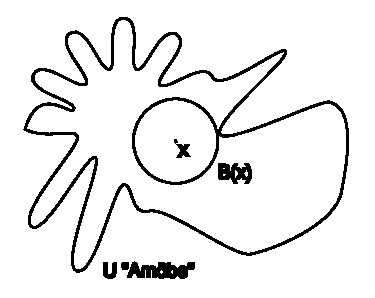
\includegraphics[scale=1]{./pic/umgeb.eps}\vspace*{-4cm}\\
Jeder (offene) $\eps$-Ball mit Mittelpunkt $x$\\
ist also Umgebung von x,\\
und "uberdies jede ''gr"o"sere'' Menge,\\
d.h. jede Menge die einen $\eps$-Ball enth"alt.
\end{definition}
\vspace*{1cm}
\begin{prop}\label{1.7}{Konvergenz via Umgebungen}\\
$x_\infty :=\lim _{n\ra\infty}x_n\eq \forall U:\mbox{\it $U$ \ul{ist Umgeb. von $x_\infty$}}\exists N\in\N:\forall n\geq N: x\in U$.
\beweis{
\item[$(\impl )$] Sei $U$ Umgebung von $x_\infty\quad\impl\exists\eps >0:B_\eps (x_\infty)\seq U$\\
\hspace*{5cm}$\impl\quad \exists N\in\N:\forall n\geq N:x_n\in B_\eps (x_\infty)\seq U$\\
\hspace*{5cm}$\impl\quad \exists N\in\N:\forall n\geq N:x_n\in U$
\item[$(\lpmi)$] Jeder $B_\eps (x_\infty)$ ist ja eh schon Umgebung von $x_\infty$
}
\end{prop}
\subsubsection{Eliminierung des Abstandsbegriffs aus der Definition der Stetigkeit}
\begin{definition}\label{1.8}\index{Stetigkeit}{Stetigkeit}\\
Seien $(X,d_X),(Y,d_Y)$ metrische R"aume, $x\in X$ und $f:X\ra Y$.\\
$f$ stetig in x :$\eq\forall\eps >0:\exists \delta >0:
\underbrace{\forall x'\in X: d_X(x,x')< \delta\impl d_Y(f(x),f(x')) < \eps }
_{f(B_\delta(x))\seq B_\eps(f(x))\eq B_\delta(x)\seq \inv{f}(B_\eps(f(x)))}$
\end{definition}

\begin{prop}\label{1.9}{Stetigkeit via Umgebungen}\\
Sei $f$ stetig in $x$ $\eq$ $\forall U$ Umgeb. von $f(x)$ ist $\inv{f}(U)$ Umgeb. von x.
\beweis{
\item[$(\impl )$] Sei $U$ Umgebung von $f(x) \implmit{\ref{1.6}}\exists\eps >0: B_\eps(f(x))\seq U\impl\\
\implmit{stetig}\exists\delta >0:B_\delta (x)\seq \inv{f}(B_\eps(f(x)))\implmit{\ref{1.6}}\inv{f}(B_\eps(f(x))) $ ist Umgeb. von x\\
$\impl$ $\mbox{da } \inv{f}(B_\eps(f(x)))\seq \inv{f}(U)\impl\inv{f}(U)\mbox{ ist Umgebung von x}$.
\item[$(\lpmi )$]
Sei $\eps >0\impl B_\eps f(x)$ ist Umgebung von $f(x) \implmit{Vorauss.}\\
 \inv{f}(B_\eps (f(x)))$ ist Umgebung von x $\implmit{\ref{1.6}}\exists\delta >0 :B_\delta (x)\seq\inv{f}(B_\eps (f(x)))$}
\end{prop}
Ob eine Funktion $f:X\ra Y$ zwischen metr. R"aumen [bzw. normierten VR's] in \ul{jedem} Punkt stetig ist (="uberall stetig/stetig) l"asst sich auch mit Hilfe des Begriffs der offenen Menge anstatt des der Umgebung beschreiben:
\begin{definition}\label{1.10}{Stetigkeit}\\
Sei $f:X\ra Y$ , X,Y metrische R"aume:\\
$f$ stetig:$\eq \forall x\in X$: f stetig in x {\small oder}\\
$f$ stetig:$\eq \forall x\in X: \forall \eps >0: \exists\delta >0: B_\delta (x)\seq \inv{f}(B_\eps(f(x)))\eq$\\
$\eq\forall x\in X \forall U \mbox{ ist Umgebung von }f(x):\inv{f}(U)$ ist Umgebung von x.
\end{definition}
\begin{definition}\label{1.11}\index{Menge!offene}{offene Menge eines metrischen Raums X}\\
$G\seq X$ hei"st \ul{offen}:$\eq \forall x\in G$: G ist Umgebung von x\\
 $[\eqmit{\ref{1.6}} \forall x\in G\exists \eps >0:B\eps (x)\seq G$ ]
\end{definition}
$\eps$ wird im Allgemeinen von x abh"angen:\\ je n"aher x am ''Rand'' von G liegt,\\ umso kleiner muss $\eps$ gew"ahlt werden.
\vspace*{-3.7cm}\\
\hspace*{10cm}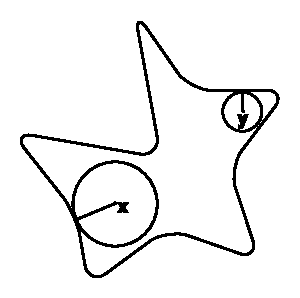
\includegraphics[scale=0.9]{./pic/1.11.eps}
\begin{prop}\label{1.12}{offene B"alle sind offene Mengen}
\beweis{
Sei $y\in B_\eps (x)\implmit{!}$ setze $\eps ':=\eps-d(x,y)$\vspace*{-1.3cm}\\
\hspace*{8.5cm}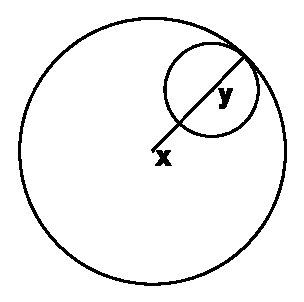
\includegraphics[scale=0.7]{./pic/ball.eps}\\
\hspace*{-0.8cm}Sei $z\in B_{\eps '}(y)\implmit{\triangle -Ungl.} d(x,z)\leq d(x,y) + \underbrace{d(y,z)}_{< \eps '}\hspace*{-0.01cm}< d(x,y) + (\eps - d(x,y))=\eps$
\vspace*{-0.3cm}
}
\end{prop}

\begin{bem}\label{1.13}{zu offenen Mengen}
\begin{enumerate}[(i)]
\item \ref{1.11} und \ref{1.12} gilt genauso f"ur normierte Vektorr"aume $(V,\norm{\_ })$
\item $\emptyset$ und X sind offen in jedem Raum\\
$\forall x\in G:$ G ist Umgebung von x\\
$\forall x\in\emptyset $: alles\footnote{{\it ex falsum quod libet}(=aus falschem folgt beliebiges) - \\ \hspace*{0.6cm}d.h. f"ur die leere Menge ist nichts zu "uberpr"ufen} $\surd$
\item offene Mengen in $\R$: 1. (a,b), 2. $\bigcup_{k=1}^\infty (a_k,b_k)$ sind schon alle (!) (ohne Beweis)
\end{enumerate}
\end{bem}
\begin{prop}\label{1.14}{(Topologische) Charakterisierung von Stetigkeit}\\
Sei $f:X\ra Y$ , $(X,d_X),(Y,d_Y)$ metrische R"aume:\\
f stetig$\eq$ $G\seq Y$ offen: $\inv{f}(G)\seq X$ offen.\\
\hspace*{5cm}\framebox{kurz: $\inv{f}$(offen) ist offen}
\beweis{
\item[$(\impl )$]Sei $G\seq Y$ offen {\small [z.z.: $\inv{f}(G)$ offen, i.e. $\forall x\in\inv{f}(G)$ ist $\inv{f}(G)$ Umg. v. x.]}\\
Sei weiters $x\in\inv{f}(G)$ d.h. $f(x)\in G$;\\
 G offen $\impl $G ist Umgebung von $f(x)\implmit{\ref{1.10}} \inv{f} (G) $ ist Umgebung von x\\
$\impl \inv{f} (G) $ ist offen.
\item[$(\lpmi )$] Sei $x\in X$ und $U$ eine Umgebung von $f(x)$\\
$\impl \exists\eps >0: B_\eps (f(x))\seq U$ au"serdem ist nach \ref{1.12} $B_\eps (f(x))$ offen\\
$\impl \inv{f}(B_\eps (f(x)))$ ist offen; wegen $f(x)\in B_\eps (f(x))$ ist f"ur $x\in\inv{f}(B_\eps (f(x)))\\
\implmit{\ref{1.11}} \inv{f}(B_\eps (f(x)))$ Umgebung von x.\\
Wegen $\inv{f}(B_\eps (f(x)))\seq \inv{f}(U)$ ist auch $\inv{f}(U)$ Umgebung von x.
}
\end{prop}

\begin{bem}\label{1.15}{zur Charakterisierung der Stetigkeit}
\begin{enumerate}[(i)]
\item Im letzten Beweisschritt: $W$ Umgebung von x und $W_1\supseteq W\impl W_1$ ist\\ Umgebung von x (klar nach \ref{1.6}).
\item Beweis analog f"ur normierte Vektorr"aume (V,$\norm{\_ }$)
\end{enumerate}
\end{bem}
\ul{\bf Zusammenfassung}:\\ Sei (X,d) ein metrischer Raum (z.B.: $A\seq\R^p$ mit $d_{(e)}$ der euklid. Metrik)\\
\begin{tabular}{|l|}\hline\\
$\bullet$ $U$ Umgebung von x $:\eq$ $\exists\eps >0:B_\eps (x)\seq U\dots$\footnotemark\\
$\bullet$ G offen :�$\eq$ G ist Umgebung jedes seiner Punkte\\
$\bullet$ $x_\infty = \lim_{n\ra\infty}x_n :\eq \underbrace{\exists N\in\N \exists n\geq N :x_N\in U_{x_\infty}}_{(x_n)_{n\in\N } \mbox{\footnotesize ist schlie"slich in } U_{x_\infty}}$\\
$\bullet$ $[ x_0$ ist HW von $(x_n)_{n\in\N} :\eq \forall N\in\N\exists n\geq n:x_N\in U_{x_0}$ ]\\
$\bullet$ f stetig in x$\eq \inv{f}(U_{f(x)})$ ist Umgebung von x; {\small oder} $\inv{f}(U_{f(x)})\supseteq U_x$.\\
\\\hline
\end{tabular}
\footnotetext{Sprache der metrischen R"aume (Zahlenwerte von Abst"ande)}\\

Auch die "ubrigen Begriffe aus der anf"anglichen Liste k"onnen ohne Verwendung einer Metrik formuliert werden -\\
\ul{\bf Ausnahmen}:\vspace*{0.3cm}\\
$\left.\begin{array}{l} Cauchy-Folge\\
Gleichm"a"sige-Stetigkeit
\end{array}\right\}\mbox{geh"oren zum Konzept der {\it Uniformen R"aume}}$\vspace*{0.3cm}\\
Wieso das ?
\begin{itemize}
\item $(x_n)_{n\in\N}$ \ul{Cauchy-Folge}\index{Cauchyfolge@{\sc Cauchy}-Folge} $:\eq \forall\eps >0\exists N\in\N :\forall N\leq n\leq m\in\N:\underbrace{d(x_n,x_m)<\eps}_{x_m\in B\eps (x_n)}\vspace*{-0.5cm}\\
\eqmit{Versuch!}\forall U$(Umgebung von $x_n$\dots{\sc hilfe!}, welches $U$?)\\
\framebox{\sc stop!} Alle $x_n$ br"auchten eine Umgebung mit gleicher Gr"o"se - aber was hei"st ''gleich gro"s'',''kleiner'',''gr"o"ser'' bei verschiedenen $x_n,x_{n_1}$ ohne Verwendung des Radius-/Abstandsbegriffs ?[bei \ul{einem} (Mittel-)Punkt x ist dies klar: $\eps_1\leq\eps_2\dots B_{\eps_1}(x)\seq B_{\eps_2}\dots U\seq U'$]
\item $f:X\ra Y$ \ul{gleichm"a"sig stetig}\index{Stetigkeit!gleichmassige@gleichm{\"a}{\ss}ige}:$\eq\forall\eps >0\exists\delta >0\forall x,x'\in X:\\ \hspace*{7cm}\underbrace{d_X(x,x')<\delta}_{x'\in B_\delta (x)}\impl \underbrace{d_Y(f(x),f(x'))<\eps}_{f(x')\in B_\eps f(x)}$\\
Wiederum: ich br"auchte f"ur \ul{alle} Umgebungen von x, mit fixer, vergleichbarer Gr"o"se von Radius $\delta$ (bzw. f"ur $f(x)$ mit Radius $\eps$ ) - das geht aber nicht ohne Abstandsbegriff !
\end{itemize}
Wir haben jetzt nun vom Teil $TC^2 (\mbox{ von } TC^4)$ die Spuren in der Analysis-VO aufgedeckt:
\begin{description}
\item T\dots{\it {\bf t}opology}\dots Umgebungen, offene Mengen\dots\ref{1.6},\ref{1.11}
\item C\dots{\it {\bf c}onvergence}\dots Konvergenz\dots\ref{1.7}
\item C\dots{\it {\bf c}ontinuity}\dots Stetigkeit\dots\ref{1.9}, \ref{1.14}
\end{description}
Wo gibt es Spuren der weiteren C's??
\begin{description}
\item C\dots{\it {\bf c}ompactness}\dots Kompaktheit\\
{\bf Satz:}{Maxima und Minima einer stet. Funktion auf einem kpt. Intervall}\\
Jede stetige, reellwertige Funktion $f$ nimmt auf einem kompakten Intervall $I=[a,b]$ ein Minimum und ein Maximum an.\\
Dahinter steckt der topologische Satz \ref{6.5}:\\ {\it Stetige Bilder kompakter Mengen} (hier $f([a,b])$) {\it sind wiederum kompakt} , und dies hei"st in $\R$ (nach {\sc Heine-Borel})  beschr"ankt und abgeschlossen;\\ beschr"ankt $\impl f([a,b])$ hat ein endliches Supremum und ein endl. Infimum;\\ abgeschlossen$\impl$ beide geh"oren zu $f([a,b])$, sind also ein maximaler und ein minimaler Funktionswert.
\newpage
\item C\dots{\it {\bf c}onnectedness}\dots ''Zusammenh"angendheit''\\
�{\bf Satz:}{\sc Zwischenwertsatz}\\
Nimmt eine stetige, reellwertige Funktion auf einem Intervall die Werte $c$ und $d$ mit $c<d$ an, so auch jeden Wert dazwischen.\\
Zur Illustration zun"achst ein \ul{Gegenbeispiel} mit einer passenden \ul{unstetigen} Funktion $f:[-1,+1]\ra\R; x\mapsto\left\{\begin{array}{l r}
x& \mbox{f"ur }-1\leq x\leq0\\
2-x&\mbox{f"ur }0 < x\leq +1
\end{array}\right.$\\
\begin{center}
\includegraphics[scale=0.7]{./pic/unstet1.eps}
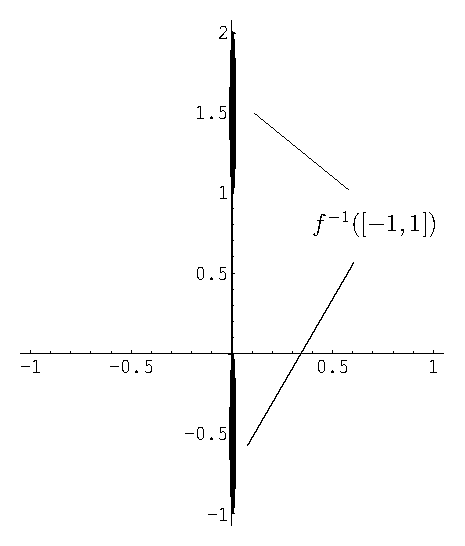
\includegraphics[scale=0.7]{./pic/unstet2.eps}
\end{center}
$f([-1,+1])=[-1,0]\cup [1,2)$\\
$f(0)=0, f(1)=1$ aber f"ur kein $x\in [-1,+1]$ ist $f(x)=\durch{2} $.
\end{description}
Das Bild $f([-1,+1])$ besteht also aus zwei getrennten St"ucken, obwohl der\\ Definitionsbereich aus einem St"uck besteht (= zusammenh"angend); offenbar ist die Unstetigkeit von $f$ die Ursache f"ur das ''Auseinanderrei"sen''.\\
Der {\sc Zwischenwertsatz} besagt nun, dass bei stetiger $f$ die Bildmenge nun aus\\ einem St"uck besteht, wenn die Definitionsmenge aus einem St"uck besteht, d.h. ein Intervall ist.\\
Dahinter steckt der topologische Satz \ref{7.3}: {\it Stetige Bilder zusammenh"angender Mengen sind zusammenh"angend.}
\newpage


\section{Topologische R"aume}
\subsection{Der 7 bis 11-fach Pfad zum Haus der Topologie}
\begin{center}
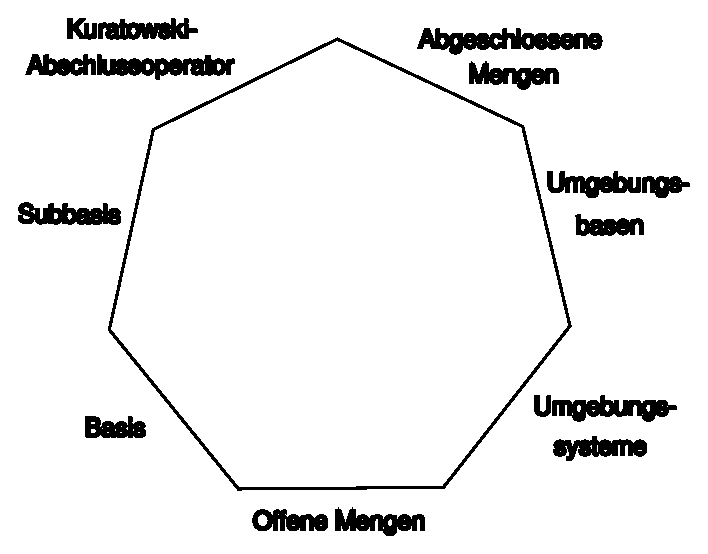
\includegraphics[scale=0.8]{./pic/topoweg.eps}
\end{center}
Es gibt verschiedene (jedoch gleichwertige) Zug"ange zum Begriff des topologischen Raumes. Ich(=Grosser Michael) habe f"ur diese Vorlesung diese 7 ausgew"ahlt.\\
Wir(=Grosser Michael) w"ahlen offene Mengen als ''unsere'' Definition.\\
{\bf Notation:} F"ur jede Menge X bezeichnet $2^X:=\{Y|Y\seq X\}$\dots die \ul{Potenzmenge} von X d.h. die Menge aller Teilmengen von X.\\
\indent Eine Teilmenge ${\mathcal F}$ von $2^X$ ist also eine ''Menge von Teilmengen'' (oft unsauber auch Familie/System von Teilmengen)
\subsubsection{Offene Mengen}
\begin{definition}\label{2.1}\index{Topologie!}\index{Topologie!offene Mengen}{Topologie}\\
\nomenclature{$\T$}{eine Topologie auf einer Menge X}%
Sei X eine Menge, eine \ul{Topologie} ist eine Teilmenge $\T$ von $2^X$ mit folgenden Eigenschaften:
\begin{description}
\item[(O1)] $\emptyset\in\T$ und $X\in\T$
\item[(O2)] $\forall G_i\in\T, i\in I\impl \bigcup_{i\in I}G_i\in\T$
\item[(O3)] $G_1\dots G_n\in\T\impl\bigcap_{i=1}^nG_i\in\T$\footnote{es w"urde reichen (O3) f"ur je zwei $G_i,G_j; 1\leq i<j\leq n\impl G_i\bigcap G_j\in\T$ zu definieren.}
\end{description}
\end{definition}

\begin{definition}\label{2.2}\index{Raum! topologischer}{Topologischer Raum}\\
Das Paar $(X,\T)$ hei"st dann \ul{topologischer Raum} (eine Menge X mit einer Topologie $\T$- oft schlampig ein topologischer Raum X z.B.: wenn klar welche Topologie gemeint ist). Die $G\in\T$ werden als $\T -$offene Mengen bezeichnet, oft auch nur offene Mengen ( "ubrigens der Buchstabe G daf"ur kommt von {\it Gebiet} einem Begriff aus der komplexen Analysis).
\end{definition}

\begin{beispiel}\label{2.3}{von Topologien}
\begin{enumerate}
\item Jeder metr. Raum (X,d) wird durch $\T =\{ G\seq X|\forall x\in G: \exists\eps >0: B_\eps (x)\seq G \}$ zum topolog. Raum z.z: O1-O3:
\beweis{
\item[(O1)] $\emptyset \in\T\surd ;\quad X\in\T \mbox{ da }\forall x\in X:\forall\eps >0: B_\eps (x)\seq X$
\item[(O2)] Sei $G_i$ offen, $i\in I$ und $x\in\bigcup_{i\in I}G_i\impl$\\
$\impl\exists i_0: x\in G_{i_0}\impl \exists\eps >0:B_\eps (x)\seq G_{i_0}\seq\bigcup_{i\in I}G_i\impl\bigcup_{i\in I} G_i$ offen
\item[(O3)] $G_1\dots G_n$ offen; und $x\in \bigcap_{i=1}^n G_i \impl\forall i\in \{ 1,\dots ,n\} :x\in G_i\impl$\\$\impl\exists\eps_1\dots\eps_n :B_{\eps_i}(x)\seq G_i\impl \eps ':=\min\{ \eps_1,\dots \eps_n\}\impl$\\$\impl B_{\eps '}(x)\seq\bigcap_{i=1}^n G_i\impl\bigcap_{i=1}^n G_i$ offen
}
\item Spezialfall von 1.: $(A,d)$ mit $A\seq\R^n, d_{eukl}$ bzw. jede Teilmenge eines normierten VR's $(V,�\norm{\_})$ und $d(x,y):=\norm{x-y}$ (\ref{1.3}).
\item diskrete Topologie von X: $\T_{diskr} =2^X$ jede Teilmenge von X\index{diskrete Topologie}\index{Topologie!diskrete}\\
''Klumpentopologie''/triviale Topologie von X: $\T_{kl} = \{ \emptyset ,X\}$\index{Klumpentopologie}\index{Topologie!Klumpen-}\\
O1-O3\dots klar
\item kofinite Topologie\index{kofinite Topologie}\index{Topologie!kofinite} einer Menge X $\T =\{ A\seq X|X\setminus$ A ist endlich$\}\cup \{\leer\}$ (O1-O3\dots PS)
\end{enumerate}
\end{beispiel}

\begin{bem}\label{2.4}{Vergleich von Topologien (mit ''$\seq$'')}\\
z.B $\T_{kl}\seq\T\seq\T_{diskr}$\\
\indent $\T_1\seq\T_2$\dots $\T_1$ ist gr"ober als $\T_2$; $\T_2$ ist feiner als $\T_1$\\
Die feinere Topologie hat �\ul{mehr} offene Teilmengen,\\
daf"ur aber \ul{kleinere} offene Mengen (i.A.) als die gr"obere.
\end{bem}

\subsubsection{Umgebungen und Umgebungssysteme}
\begin{definition}\label{2.5}\index{Umgebungssystem}\index{Topologie!Umgebungssystem}{Umgebungssystem von x}\\
Sei $(X,\T )$ ein topologischer Raum und $U\seq X$; $x\in X$,\\
dann hei"st U: \ul{($\T$-)Umgebung von x}:$\eq\exists G\seq\T : x\in G\seq U$.
$$\umg{U}{x}^{(\T )} :=\{ U\in\T |U\mbox{ ist Umgebung von x}\}\dots\mbox{hei"st \ul{Umgebungssystem von x}}$$
\end{definition}
\begin{prop}\label{2.6}{Charakterisierung offener Mengen durch Umgebungen}\\
Sei $(X,\T)$ ein topologischer Raum und $G\seq X$: G ist genau dann offen, wenn G Umgebung all seiner Punkte ist.[G ($\T$-)offen $\eq \forall x\in G: G\in\umg{U}{x}$]
\begin{description}
\item[\bf Beweis:]
\item[$(\impl )$]G offen; $x\in G\impl x\in G\seq G \impl G\in\umg{U}{x}$
\item[$(\lpmi )$] Sei $x\in G \implmit{Vorauss.} G\in\umg{U}{x}\implmit{\ref{2.5}}\exists H_x\in\T :x\in H_x\seq G$;\\
$G=\bigcup_{x\in G}\{ x\}$\footnote{G ist klarerweise die Vereinigung all seiner Punkte}$ \seq \bigcup_{x\in G}H_x\seq G\impl G = \bigcup_{x\in G} H_x\in\T$ d.h. G ist offen\hfill\fertig
\end{description}
\end{prop}

\begin{kor}\label{2.7}Jede Umgebung U von x enth"alt eine \ul{offene} Umgebung V von x.
\beweis{Nimm f"ur V das G aus \ref{2.5}; $x\in G\seq U$; $G\in\T\implmit{\ref{2.6}} G\in\umg{U}{x}$
}
\end{kor}

\begin{satz}\label{2.8}{\sc Grundeigenschaften von Umgebungssystemen}\\
Sei $(X,\T )$ topologischer Raum; f"ur die Umgebungssysteme $\umg{U}{x}$ gilt:
\begin{enumerate}[(U1)]
\item $\forall U\in\umg{U}{x}:x\in U[\impl U\neq\leer]$
\item $\forall U_1,U_2\in\umg{U}{x}:U_1\cap U_2\in\umg{U}{x}$
\item $\forall U\in\umg{U}{x}: V\supseteq U: V\in \umg{U}{x}$\footnote{Die Eigenschaften U1-U3 definieren einen ''\ul{Filter}'' $\umg{U}{x}$}
\item $\forall U\in\umg{U}{x}\exists V\in\umg{U}{x}; V\seq U: \forall y\in V: U\in\umg{U}{y}$
\end{enumerate}
vergleiche in metr. R"aumen $\underbrace{B_\eps (x)}_U ,\delta\leq\eps '=\frac{\eps}{2}<\eps\impl\forall y\in \underbrace{B_{\eps '}(x)}_V:\underbrace{B_\delta (y)\seq B_\eps (x)}_{\mbox{\scriptsize U ist Umgebung von y}}\vspace*{-0.3cm}$\vspace*{-0.2cm}
\beweis{
\item[(U1)] $U\in\umg{U}{x}\implmit{\ref{2.5}}\exists G \mbox{(offen)} :x\in G\seq U\impl x\in U$
\item[(U2)] Sei $U_1, U_2\in\umg{U}{x}\implmit{\ref{2.5}}\exists G_1, G_2\mbox{ offen }; x\in G_1\seq U_1, x\in G_2\seq U_2\implmit{O3}\\
\indent x\in\underbrace{G_1\cap G_2}_{\mbox{\scriptsize offen}}\seq U_1\cap U_2\implmit{\ref{2.5}} U_1\cap U_2 \in \umg{U}{x}$\vspace*{-0.5cm}
\item[(U3)] $U\in\umg{U}{x}; V\supseteq U\implmit{\ref{2.5}}\exists G\mbox{ offen}:x\in G\seq U\seq V\impl V\in\umg{U}{x}$
\item[(U4)] $U\in\umg{U}{x}\implmit{\ref{2.5}}\exists G\mbox{ offen}:x\in G\seq U;\mbox{ setze } V:=G\implmit{\ref{2.6}}$\\
V ist Umgebung von jedem $y\in V$. Insbesonders gilt dies f"ur $y:=x\impl\\ V\in \umg{U}{x}=\umg{U}{y}; U\supseteq V\implmit{U3} U\in \umg{U}{y}$
}
\end{satz}

\begin{lemma}\label{2.9}{(U4+) folgt aus U4 und U3}\\
Sei X eine Menge und $\forall x\in X$ sei $\umg{V}{x}$ ein Mengensystem auf X ($\umg{V}{x}\seq 2^X$), das U3 und U4 erf"ullt. Dann erf"ullen die $\umg{V}{x}$ auch:
\begin{description}
\item[(U4+)] $\forall U\in \umg{V}{x}\exists V\in\umg{V}{x}: V\seq U \wedge\forall y\in$\framebox{$V\in\umg{V}{y}$}
\end{description}
\beweis{ Sei $U\in\umg{V}{x}$ setze
\begin{equation}
W:=\{ y\in U|U\in\umg{V}{y}\} \label{star1}
\end{equation}
\item Wir zeigen: W erf"ullt die Anforderungen an V in (U4+):
\item[($W\in\umg{V}{x}$)] denn $\implmit{(U4)}\exists V\in\umg{V}{x}, V\seq U: \underbrace{\forall y\in V:U\in\umg{V}{y}}_{\mbox{\ref{star1}}\impl V\seq W}\implmit{U3} W\in\umg{V}{y}$\vspace*{-0.5cm}
\item[($W\seq U$)] gilt per definitionem
\item[($W\in \umg{V}{y}$)] Sei $y\in W\impl  U\in \umg{V}{y}\implmit{U4}\exists V\seq U, V\in\umg{V}{y}\underbrace{\forall z\in V}_{\mbox{$|\hspace*{-0.03cm}|$}}:U\in\umg{V}{z}\vspace*{-0.45cm}\\
\hspace*{6.75cm}\implmit{\mbox{\ref{star1}}} z\in W\Longrightarrow V\seq W\\
\hspace*{9.3cm}\implmit{U3} W\in \umg{V}{y}$
}
\end{lemma}
\begin{satz}\label{2.10}{\sc Offene Mengen "uber Umgebungssysteme}\\
Sei X eine Menge und f"ur jedes $x\in X$ sei ein nichtleeres Mengensystem $\umg{V}{x}$ das (U1-U4) erf"ullt. Dann ist $\T =\{ G\seq X|\forall x\in G: G\in\umg{V}{x}\}$[nach \ref{2.6}] eine Topologie auf X. F"ur jedes X ist das Umgebungssystem $\umg{U}{x}^\T =\umg{U}{x}$ genau das gegebene $\umg{V}{x}$. $\T$ ist die einzige Topologie mit dieser Eigenschaft.\vspace*{-0.3cm}
$$\xymatrix{\T (O1)-(O3) \ar@{=>}@/^3pc/[r]^{\ref{2.5},\ref{2.8}}&\umg{U}{x}^\T (U1)-(U4) \ar@{=>}@/^3pc/[l]^{bij,\ref{2.10}}}$$\vspace*{-1.5cm}
\beweis{
\item[(O1)] $\leer\in\T :\surd$ , da $\forall x\in\leer\dots$\\
$\forall x\in X\exists �U\in\umg{V}{x}\implmit{U3} X\in\umg{V}{x}\impl X\in\T$
\item[(O2)] Sei $(G_i)_{i\in I}\in\T$ und sei $x\in\bigcup_{i\in I}G_i\impl\exists i_0\in I: x\in G_{i_0}\implmit{Def.v.\T} G_{i_0}\in\umg{V}{x}\implmit{(U3)}\bigcup_{i\in I} G_i\in\umg{V}{x}\impl\bigcup_{i\in I}G_i\in\T$.
\item[(O3)] Seien $G_1\dots G_n\in\T$ und sei\footnote{o.B.d.A $\bigcap_{i=1}^n G_i \neq\leer$- wenn doch dann ist $\leer\in\T$(per Def.)- also nichts zu zeigen} $x\in\bigcap_{i=1}^n G_i\in\T\impl\forall 1\leq i\leq n:x\in G_i\impl \forall 1\leq i\leq n: G_i\in\umg{V}{x}\implmit{U2,Induktion}\bigcap_{i=1}^n G_i \in\umg{V}{x}\impl \bigcap_{i=1}^n G_i \in\T$
\item[($\umg{U}{x}^\T=\umg{V}{x}$)] D.h. sei $U\seq\umg{U}{x}^\T\implmit{\ref{2.5}}\exists G\in\T:x\in G\seq U(\seq \T)\implmit{Def.v.\T}\\
\exists G:G\seq (U\cap G)\in \umg{V}{x}\implmit{(U3)} U\in\umg{V}{x}\impl \umg{U}{x}^\T\seq\umg{V}{x}$\\
Sei $U\in\umg{V}{x}\implmit{\ref{2.9},(U4+)}\exists V\in \umg{V}{x} , V\seq U\underbrace{\forall y\in V: V\in\umg{V}{y}}_{V\in\T (Def.v.\T )}\implmit{(U1)}x\in V(\T \mbox{-offen}):V\seq U\implmit{\ref{2.5}}U \mbox{(ist Umgebung von x) }U\in \umg{U}{x}^\T\impl \umg{U}{x}^\T\supseteq \umg{V}{x}$\\
$\umg{U}{x}^\T = \umg{V}{x}$
\item[\ul{Eindeutigkeit:}]Sei $\T '$ nun ebenfalls eine Topologie auf X mit $\umg{U}{x}^{\T '}=\umg{V}{x}$.\\ Wegen \ref{2.6} ist $\T = \T '$:
$$\xymatrix{
U\in\T \eqmit{\ref{2.6}}\forall x\in U:&\hspace*{-1cm}U\in\umg{U}{x}^\T \ar@{=}@/^0.8cm/[dr]\vspace*{-1cm}\\
{}&&\umg{V}{x}\\
U\in\T ' \eqmit{\ref{2.6}}\forall x\in U:&\hspace*{-1cm}U\in\umg{U}{x}^{\T '} \ar@{=}@/_0.8cm/[ur]}$$\vspace*{-0.5cm}
}
\end{satz}

\subsubsection{Umgebungsbasen}

\begin{definition}\label{2.11}\index{Umgebungsbasen}\index{Topologie!Umgebungsbasen}{Umgebungsbasen}\\
Sei (X,$\T$) ein topologischer Raum und $x\in X$.\\
Ein Teilsystem $\umgbas{W}{x}$ von $\umg{U}{x}$ hei"st \ul{Umgebungsbasis (bez. $\T$ bei x)}, wenn gilt:
$$\forall U\in\umg{U}{x}\exists W\in\umgbas{W}{x}:(x\in )W\seq U$$
\end{definition}

\begin{satz}\label{2.12}{\sc Grundeigenschaften von Umgebungsbasen}\\
Sei (X,$\T$) ein topologischer Raum, f"ur ein System $\umgbas{W}{x} (x\in X)$ von Umgebungsbasen gilt dann:
\begin{description}
\item[(UB1)] $\forall W\in\umgbas{W}{x}:x\in W$[$\impl W\neq\leer$]
\vspace*{-1.5cm}\item[(UB2)] $\forall W_1,W_2\in\umgbas{W}{x}\exists W_3\seq W_1\cap W_2$\footnote{(UB1) und (UB2) sind auch die Grundeigenschaften(FB1) und (FB2) einer \ul{Filterbasis}}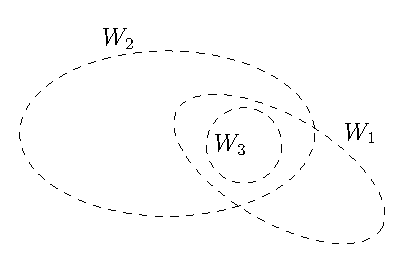
\includegraphics[scale=0.7]{./pic/umgbas.eps}\\
\item[(UB4)] $\forall W\in \umgbas{W}{x}\exists V\in\umgbas{W}{x}:V\seq W\in\umgbas{W}{x} \wedge\forall y\in V\exists W_y\in\umgbas{W}{y}:W_y\seq W$
\end{description}
\beweis{
\item[(UB1)] =(U1)
\item[(UB2)] $W_1,W_2\in\umgbas{W}{x}\seq \umg{U}{x}\implmit{(U2)} W_1\cap W_2\in \umg{U}{x}\implmit{\ref{2.11}}\exists W_3\in \umgbas{W}{x}:W_3\seq W_1\cap W_2$
\item[(UB4)] $W\in\umgbas{W}{x}\impl W\in\umg{U}{x}\implmit{(U4)}\exists V_1\in \umg{U}{x},V_1\seq W\forall y\in V_1 : W\in\umg{U}{y}\\
\hspace*{3cm}\implmit{\ref{2.11}}\exists V\in \umgbas{W}{x}:V\seq V_1\\
\hspace*{3cm}\implmit{}\exists V\in \umgbas{W}{x}: V\seq W\wedge \forall y\in V:W\in \umg{U}{y}\\
\hspace*{3cm}\implmit{\ref{2.11}}\exists V\in \umgbas{W}{x}:V\seq W\wedge \forall y\in V\exists W_y\in\umgbas{W}{y}: W_y\seq W$
}
\end{satz}


\begin{satz}\label{2.13}{\sc Topologie "uber Umgebungsbasis}\\
Sei X eine Menge und f"ur jedes $x\in X$ sei ein nichtleeres Mengensystem $\umgbas{V}{x}\seq 2^X$ gegeben, das (UB1),(UB2) und (UB4) erf"ullt. Dann definiert:
$$\umg{U}{x}=\{ U\seq X |\exists V\in\umgbas{V}{x}:(x\in )V\seq U\}$$
Ein Umgebungssystem f"ur eine Topologie $\T$ auf X. $\umgbas{V}{x}$ ist Umgebungsbasis f"ur $\T$ und $\T$ ist die einzige Topologie mit dieser Eigenschaft.
\beweis{
\item[(U1)] $U\in\umg{U}{x}\impl \exists V\in\umgbas{V}{x}:V\seq U;\\\hspace*{1.5cm} \implmit{(UB1)} x\in V\impl x\in U$
\item[(U2)] $\forall U_1, U_2\in\umg{U}{x}\impl\exists V_i\in\umgbas{V}{x}:x\in V_i \in U_i$\hspace*{1cm}$(i\in\{ 1,2\})\\
\hspace*{2.8cm}\implmit{(UB2)}\exists V_3\in\umgbas{V}{x}: V_3\seq V_1\cap V_2\seq U_1\cap U_2\\
\hspace*{3cm}\implmit{} U_1\cap U_2\in \umg{U}{x}$
\item[(U3)] $U\seq\umg{U}{x}, U_1\supseteq U\impl\exists V\in\umgbas{V}{x}:V\seq U\seq U_1\\
\hspace*{3cm}\impl U_1\in \umg{U}{x}$
\item[(U4)] $U\in\umg{U}{x}\impl\exists W\in\umgbas{V}{x}:(x\in )W\seq U\\
\hspace*{1.3cm}\implmit{(UB4)}\exists V\in\umgbas{V}{x}: V\seq W\wedge \forall y\in V \underbrace{\exists W_y\in\umgbas{V}{y}: W_y\seq W}_{\eq W\in\umg{U}{y}}\vspace*{-0.5cm}\\
\hspace*{3.55cm}${\footnotesize \mbox{$\bigcap\hspace*{-0.06cm}\bf |$}}$\\
\hspace*{1.6cm}\implmit{}\exists V\in\umg{U}{x}:V\seq U\et\forall y\in V:U\in\umg{U}{y}$
\item F"ur jedes x ist $\umgbas{V}{x}\seq \umg{U}{x}$, per definitionem von $\umg{U}{x}$ ist $\umgbas{V}{x}$ Umgebungsbasis von x. Offenbar ist $\umg{U}{x}$ das einzige Umgebungssystem, f"ur das $\umgbas{V}{x}$ Umgebungsbasis ist. Somit ist $\T$ auch eindeutig.}
\end{satz}
\begin{beispiel}\label{2.14}{von Umgebungsbasen}
\begin{enumerate}
\item Offene Umgebungen:\\ nach \ref{2.7}\footnote{$\forall x\in U: U\in \umg{U}{x}:\exists V offen\in \umg{U}{x}:x\in V\seq U$} bilden die offenen Umgebungen eine Umgebungsbasis.
\item metrische R"aume:\\
Sei (X,d) ein metrischer Raum, $x\in X$; sei $\umgbas{V}{x}:=\{ B_\eps (x)|\eps >0\}$\\
(UB1) $x\in B_\eps (x) \surd $\\
(UB2) $W_1=B_{\eps_1} (x),W_2 = B_{\eps_2} (x), W_3=B_{\min\{\eps_1,\eps_2\}} (x)$, d.h. $W_3 = W_1\cap W_2$
(UB4) F"ur gegebenes $W=B_{\eps} (x)$ ist auch $V=B_{\frac{\eps}{2}} (x)\in\umgbas{V}{x}$\\
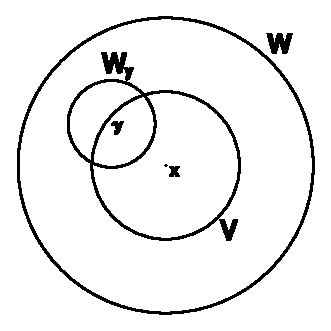
\includegraphics[scale=0.8]{./pic/ub4.eps}\vspace*{-4.1cm}\\
\hspace*{6.5cm}\vspace*{0.1cm}$V\seq W$ und $\forall y\in V$ ist\\
\hspace*{6.5cm}\vspace*{0.1cm}$W_y = B_\frac{\eps}{2} (x)\seq B_{\eps} (x)=W$\\
\hspace*{6.5cm}\vspace*{0.1cm}[nach $\triangle$-Ungleichung]\\
\hspace*{4.5cm}\vspace*{0.1cm}Die offenen B"alle $B_{\eps} (x)$ bilden also eine\\
\hspace*{4.5cm}\vspace*{0.1cm}Umgebungsbasis f"ur die von der Metrik erzeugte\\
\hspace*{4.5cm} Topologie.\\
\item Die {\sc Niemytzki}-Topologie\index{Niemytzki@{\sc Niemytzki}-Topologie}\index{Topologie!Niemytzki@{\sc Niemytzki}-} auf oberer Halbebene:\\
Sei $X:=\{ (x,y)\in\R^2|y\geq 0\}$\\
es geben die $p=(a,b)\in X$\\ eine Umgebungsbasis an.\\
$b>0$ dann $\umg{W}{p}:=\{B_{\eps} (p)|b\geq\eps>0 \}$\\
$b=0$ dann $\umg{W}{p}:=\{C_\eps(p)|\eps >0\}$ mit\\ $C_\eps (p):=\{B_\eps (m)|m=(a,\eps)\}\cup\{ p\}$\\
Ist eine Umgebungsbasis $\stackrel{\ref{2.13}}{\leadsto}$ Niemytzki-Topologie.\\
\vspace*{-5.5cm}\\ \hspace*{9cm}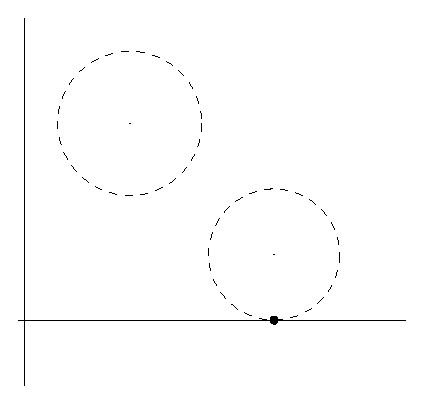
\includegraphics[scale=0.7]{./pic/niemytzkiright.eps}\\

\end{enumerate}
\end{beispiel}
\begin{bem}\label{2.15}\ul{Schema}\\
Wir haben nun bereits zweimal einen weiteren Zugang zum Haus der Topologie ge"offnet, ausgehend von einem bereits vorhandenen Zugang. Dabei sind wir nach folgendem Schema vorgegangen:
\begin{enumerate}
\item Es gibt einen Ausgangsbegriff $\cal A$, der durch Axiome $(A1)-(Aj)$ definiert ist.
\item F"ur ein gegebenes Objekt vom Typ $\cal A$ definiere wir einen weiteren Begriff $\cal B$
\item Wir zeigen f"ur $\cal B$ gewisse Grundeigenschaften $(B1)-(Bk)$.
\item Wir ernennen jetzt $(B1)-(Bk)$ zu neuen Axiomen und betrachten Objekte, die $(B1)-(Bk)$ erf"ullen (unabh"angig von $\cal A$). Ausgehend von einem solche $\cal B$-Objekt \ul{\it konstruieren} wir ein Objekt, das $(A1)-(Aj)$ erf"ullt und zeigen, dass die Konstruktion von 2. wiederum zum urspr"unglichen $\cal B$-Objekt zur"uckf"uhrt; au"serdem ist die durch das $\cal A$-Objekt bestimmte Topologie eindeutig.
\end{enumerate}
bisher:\\
\begin{tabular}{cll|rl}
1.&Topologie $\T$ (O1)-(O3)&\ref{2.1}&Umgebungssysteme $\umg{U}{x}$&\ref{2.5},\ref{2.8}\\
2.&Umgebungssysteme $\umg{U}{x}$&\ref{2.5}&Umgebungsbasen $\umg{W}{x}$&\ref{2.11}\\
3.&$(U1)-(U4)$&\ref{2.8}&$(UB1),(UB2),(UB4)$&\ref{2.12}\\
4.& Gegeben $\umg{V}{x}$mit $(Ui)$ $\leadsto$ $\T$&\ref{2.10}& Gegeben $\umg{V}{x}$ und $(UBj)$ $\leadsto \umg{U}{x}$&\ref{2.13}
\end{tabular}
\end{bem}

\subsubsection{Basis}
\begin{definition}\label{2.16}\index{Topologie!Basis}\index{Basis}{Basis}\\
Sei $(X, \T )$ ein topologischer Raum: Eine Teilfamilie $\B$ von $\T$ hei"st \ul{Basis f"ur $\T$}, wenn jedes $G\in \T$ als Vereinigung $\bigcup_{i\in I}B_i$ $(B_i\in\B)$ geschrieben werden kann (hierbei sei $\bigcup_{i\in\leer}B_i$:=$\leer$).
\end{definition}
\begin{bem}\label{2.17}{\dots oder dazu "aquivalent:}\\
$$\forall G\in\T\forall x\in G\exists B_x\in\B: x\in B_x\seq G$$
\beweis{
\item[$(\impl )$] $G=\bigcup_{i\in I}B_i , x\in G\impl \exists i_0\in I: x\in B_{i_0}\seq \bigcup_{i\in I}B_i =G$
\item[($\lpmi$)] $G=\bigcup_{x\in G}B_x$ (vgl. Beweis \ref{2.6}) oder $G=\leer$
}
\end{bem}

\begin{satz}\label{2.18}{\sc Grundeigenschaften einer Basis $\B$ f"ur eine Topologie $\T$}
Sei (X,$\T$) ein topologischer Raum, und $\B$ eine Basis f"ur $\T$ Dann gilt:
\begin{description}
\item[(B1)] $\bigcup_{B\in\B}B=X$
\item[(B3)] $\forall B_1,B_2\in\B \forall x\in B_1\cap B_2\exists B_3\in\B :x\in B_3\seq B_1\cap B_2$
\end{description}
\beweis{
\item[(B1)] $X�\in\T\impl X=\bigcup_{i\in I}B_i\seq\bigcup_{B\in\B}B=X$
\item[(B3)] $B_1,B_2\in\B, x\in B_1\cap B_2\implmit{(O3)}B_1\cap B_2 \mbox{offen}\\
\implmit{\ref{2.16}}\exists B_3\in\B :x\in B_3\seq B_1\cap B_2$
}
\end{satz}
\begin{satz}\label{2.19}{\sc Topologie "uber Basen}\\
Sei X eine Menge und $\B$ ein Teilsystem von $2^X$, das (B1) und (B3) erf"ullt. Dann definiert
$$\T :=\{\bigcup_{i\in I}B_i|B_i \in\B\}$$ eine Topologie auf X; $\B$ ist Basis f"ur $\T$ und $\T$ ist die einzige Topologie mit dieser Eigenschaft.
\beweis{
\item[(O1)] $\bigcup_{i\in\leer}B_i=\leer \in\T , \bigcup_{B\in\B}B=X\in\T$\vspace*{-0.7cm}\\
\item Vereinigungen von Vereinigungen sind Vereinigungen:\vspace*{-0.9cm}\\
\item[(O2)] $G_i\in\T$ und $i\in I\impl G_i=\bigcup_{i_j\in J_i}B_{i_j}\\
\impl \bigcup_{i\in I}G_i =\bigcup_{i\in I}\bigcup_{i_j\in J_i}B_{i_j}\in\T$\vspace*{-0.7cm}\\
\item Vereinigungen von Durchschnitten sind Vereinigungen:\vspace*{-0.9cm}\\
\item [(O3)] $G_1\dots G_n\in\T\impl G_i=\bigcup_{i_j\in J_i}B_{i_j}\\
\impl \bigcap_{i=1}^n G_i =\bigcap_{i=1}^n\bigcup_{i_j\in J_i} B_{i_j}=\bigcup_{\hspace*{-0.45cm}\mbox{\scriptsize $\left.\begin{array}{c}i_j\in J_i\\i=1\dots n \end{array}\right.$}}\hspace*{-0.45cm} B_{1_j}\cap\dots\cap B_{n_j}$\\
Ist nun $x\in B_{1_j}\cap\dots\cap B_{n_j}$, so liefert (B3) ein $B_x$ mit $x\in B_x\seq B_{1_j}\cap\dots\cap B_{n_j}$ (Induktion!). Daher ist $B_{j_1}\cap\dots\cap B_{j_n}=\bigcup_{x\in B_{j_1}\cap\dots\cap B_{j_n}}B_x\in\T\\
\implmit{(O2)} \bigcap_{i=1}^n G_i\in\T$.
\item $\B$ ist Basis von $\T$ direkt nach der Definition von $\T$. Jede Topologie $\T '$, f"ur die $\B$ eine Basis ist, besteht genau aus den $\bigcup_{i\in I}B_i$ und ist somit gleich $\T$.
}
\end{satz}

\subsubsection{Subbasis}

\begin{definition}\label{2.20}\index{Topologie!Subbasis}\index{Subbasis}{Subbasis}\\
Sei (X,$\T$) ein topologischer Raum: Eine Teilfamilie $\Sb$ von $\T$ hei"st \ul{Subbasis f"ur $\T$}, wenn die Familie aller $\bigcap_{i=1}^n S_i$ mit $S_i\in\Sb$ eine Basis f"ur $\T$ bildet, d.h. wenn jedes $G\in\T$ als
$$\bigcup_{i\in I}\bigcap_{j_i=1}^{n_i}S_{j_i}$$
geschrieben werden kann ($\bigcap_{i\in\leer}S_i:=X$).{\scriptsize (Der Schnitt von nichts gibt alles)}
\end{definition}

\begin{satz}\label{2.21}{\sc Grundeigenschaften einer Subbasis}\\
$[$keine!! Leute, die $\bigcap_{i\in\leer}S_i :=X$ nicht m"ogen, verwenden $(S1) X\in \Sb$ $]$
\end{satz}

\begin{satz}\label{2.22}{\sc Basen "uber Subbasen}\\
Sei (X,$\T$) ein topologischer Raum und $\Sb$ ein Teilsystem von $2^X$ das (S1) erf"ullt, dann ist $\B :=\{ \bigcap_{i=1}^n S_i : S_i\in\Sb \}$ eine Basis d.h. erf"ullt (B1) und(B3).
\beweis{Im Proseminar Bsp. 17}
\end{satz}

$$\xymatrix@R=-0.1cm{
\Sb\ar@{~>}[r]^{\bigcap_{i=1}^n} 	&	 \B\ar@{~>}[r]^{\bigcup_{i\in I}} 	&	 \T\\
{\bigcap_{i=1}^0 S_i=X} 				
								&
{\left.\begin{array}{c}(B1) X \\
(B3) \bigcap_{i=1}^n\\
\leer :=\bigcup_{i\in\leer}B_i\end{array}\right.}
							 	&
{\left.\begin{array}{c}(O1)\leer , X\\
(O2)\bigcup_{i\in I}\\
(O3)\bigcup_{i=1}^n\end{array}\right.}
}$$
\begin{beispiel}\label{2.23}{von Subbasen und Basen}
\begin{enumerate}
\item Produkttopologie\index{Produkttopologie}\index{Topologie!Produkt-}\\
Seien $(X_i,\T_i)_(i\in I)$ topolog. R"aume, wir definieren auf $X=\prod_{i\in I}X_i=\{ (x_i)_{i\in I}:x_i\in X_i\}$ die Produkttopologie $\T =\prod_{i\in I}\T_i$ als die von der Subbasis:\\
$\Sb =\{ S=\prod_{i\in I}Y_i:Y_i=X_i \mbox{ $\forall i$ au"ser einem bel. $i_0$ f"ur dieses sei } Y_{i_0}\in \T_{i_0}\}$\\
Wie sehen endliche Durchschnitte von Mengen aus $\Sb$ aus ?\\
\hspace*{9.5cm}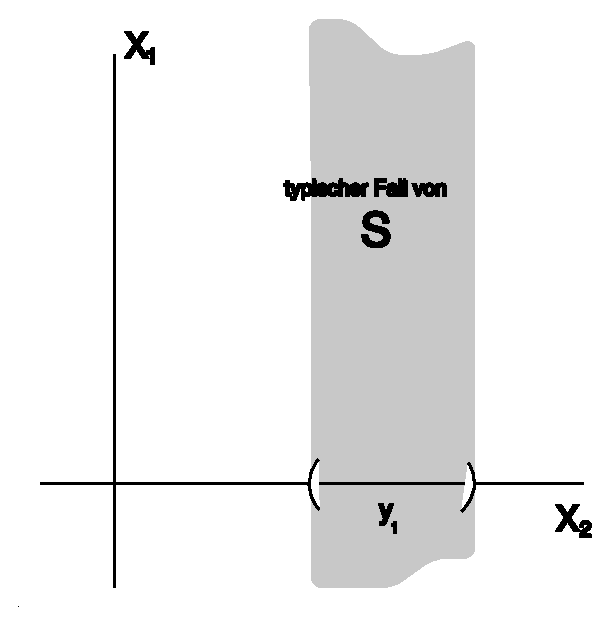
\includegraphics[scale=0.5]{./pic/subbasis.eps}\vspace*{-5cm}\\
Ist I endlich:\\
typischerweise so: $Y_1\times\dots\times Y_n$ $(Y_i\in\T_i)$\\
also n-dimensionale Quader/Intervalle\\
Sei I unendlich: dann sind es Intervalle $\prod_{i\in I}Y_i$\\
bei denen �\ul{endlich} viele $i$ das $Y_i$ von $X_i$ verschieden ist,\\
 f"ur alle anderen (= ''fast alle'') ist $Y_i=X_i$\\
z.B: Folgenr"aume $\R^\N$ diese ''Quader'' sind\\
f"ur $|I|$\footnote{Kardinalit"at}$ =\aleph_0$ sehr ''gro"s''.\\
Sie bilden eine Basis f"ur die Produkttopologie.\\
Daher sind auch die offenen Mengen bez"uglich $\T$ sehr gro"s.
\item Boxtopologie\\
Seien ebenfalls $(X_i,\T_i)_{(i\in I)}$ topologische R"aume, wir definieren auf $X=\prod_{i\in I}X_i=\{ (x_i)_{i\in I}:x_i\in X_i\}$ die Basis: $\B_{box}=\{ \prod_{i\in I}Y_i|\forall i\in I:\underbrace{Y_i\mbox{ (offen)}\seq X_i}_{Y_i\seq\T_i}\}$ der Boxtopologie $\T_{box}$\\
da $\B_{box}\seq \B_{prod}$ $\impl$ Boxtopologie feiner als Produkttopologie; wenn I endlich gibt es keinen Unterschied zwischen $\B_{prod}$ und $\B_{box}$.\\
Nachteil im Unendlichdimensionalen von $\B_{box}$\footnote{($\R^\N,\T_{box}$) ist kein topologischer VR}: $\durch{n}\cdot (1,1,\dots)\nrightarrow 0$ wohl aber in $\T_{prod}$.

\end{enumerate}
\end{beispiel}

\subsubsection{Abgeschlossene Mengen}

\begin{definition}\label{2.24}\index{Menge!abgeschlossene}\index{Topologie!abgeschlossene Mengen}{Abgeschlossene Mengen}\\
Sei (X,$\T$) topologischer Raum, $A\seq X$:\\
A hei"st \ul{$(\T -)$abgeschlossen} :$\eq X\setminus A$ offen (d.h. $X\setminus A\in\T$)
\end{definition}

\begin{satz}\label{2.25}{\sc Grundeigenschaften abgeschlossener Mengen}\\
Sei (X,$\T$) topologischer Raum, $\A$ sei die Familie der $\T$-abgeschlossenen Mengen. Dann gilt:
\begin{description}
\item[(A1)] $\leer\in\A ,X\in\A$
\item[(A2)] $A_i\in\A$ mit ($i\in I$) $\impl \bigcap_{i\in I}A_i\in\A$
\item[(A3)] $A_1\dots A_n\in\A\impl \bigcup_{i=1}^nA_i\in\A$
\end{description}
\beweis{
\item[(A1)] $X\setminus\leer = X\in\T\impl \leer\in\A$\\
$X\setminus X=\leer\in\T \impl X\in\A$
\item[(A2)] $(A_i)_{i\in I}\in\A\impl (A_i)^c\in\T (i\in I)\implmit{(O2)}\bigcup_{i\in I}(A_i)^c\in \T\\
\hspace*{2.2cm}\impl\bigcap_{i\in I}A_i=(\bigcup_{i\in I}A_i)^{cc}=(\bigcup_{i\in I}(A_i)^c)^c\in \A$
\item[(A3)] $A_1\dots A_n\in\A\impl A_1^c\dots A_n^c\in\T\bigcup_{i=1}^n(A_i)^c\in\T\\
\hspace*{2.6cm} \impl\bigcup_{i=1}^nA_i=(\bigcup_{i=1}^nA_i)^{cc}=(\bigcap_{i=1}^n(A_i)^c)^c\in\A$
}
\end{satz}

\begin{satz}\label{2.26}{\sc Topologie "uber Abgeschlossene Mengen}
\beweis{PS}
\end{satz}

\subsubsection{Inneres, "Au"seres und Rand}

Sei hier immer (X,$\T$) ein topologischer Raum und $A\seq X$ und $x\in X$

Aussagen "uber eine Teilmenge A von X :\\
\hspace*{10cm}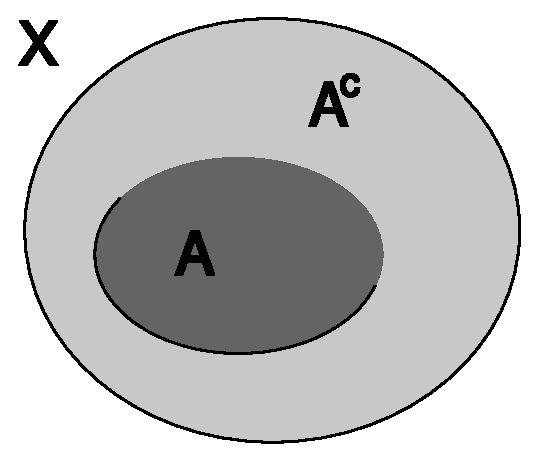
\includegraphics[scale=0.4]{./pic/AAc.eps}\vspace*{-2.7cm}\\
$A\seq X\dots\dots$ mengentheoretisch: $A$\\
\hspace*{6cm} $A^c$\\
\hspace*{2.6cm}topologisch: Inneres von A\\
\hspace*{4.85cm}"Au"seres von A\\
\hspace*{4.85cm}Rand von A\vspace*{0.1cm}\\
\hspace*{-0.2cm}$\left.\begin{array}{l}
\mbox{innen: Punkte die (mind.) eine dunkelgraue Umg. haben}\\
\mbox{au"sen: Punkte die (mind.) eine hellgraue Umg. haben}
\end{array}\right\}$\vspace*{-0.8cm}\\
\hspace*{11cm}{\scriptsize Punkte die eine {\it einf"arbige}}\vspace*{-0.2cm}\\
\hspace*{11cm}{\scriptsize Umgebung haben}\vspace*{0.15cm}\\
Rand: Punkte die nur {\it ''zweif"arbige''} Umgebungen besitzen

\begin{definition}\label{2.27}\index{Innerer Punkt}\index{Ausserer Punkt@\"Au{\ss}erer Punkt }\index{Randpunkt}{Innerer Punkt, "Au"serer Punkt, Randpunkt} \index{Inneres $\inn{A}$} \index{Ausseres@\"Au{\ss}eres $\ext{A}$} \index{Rand $\bd{A}$}
\begin{enumerate}
\item x ist Innerer Punkt von A:$\eq (\exists U\in\umg{U}{x}: U\seq A)\eq (\exists U\in \umg{U}{x}:U\cap A^c=\leer )$\vspace*{-0.9cm}\\
\item x ist "Au"serer Punkt von A:$\eq (\exists U\in\umg{U}{x}: U\seq A^c)\eq (\exists U\in\umg{U}{x}:U\cap A=\leer )$\vspace*{-0.9cm}\\
\item x ist Randpunkt von A:$\forall U\in\umg{U}{x}: U\cap A\neq\leer \et U\cap A^c\neq\leer$\vspace*{-0.9cm}\\
\end{enumerate}
$\inn{A} = \mbox{int}(A) :=\{ x\in X: x \mbox{ ist Innerer Punkt von A}\}\eq\\
\eq\{x\in X:\exists U\in\umg{U}{x}: U\cap A^c=\leer\}\eq\{ x\in X:\exists U\in\umg{U}{x}:U\seq A\}\vspace*{0.2cm}$\\
$\ext{A} :=\{ x\in X: x \mbox{ ist "Au"serer Punkt von A}\}\eq\\
\eq\{x\in X:\exists U\in\umg{U}{x}: U\cap A=\leer\}\eq\{ x\in X:\exists U\in\umg{U}{x}:U\seq A^c\}\vspace*{0.2cm}$\\
$\bd{A} :=\{ x\in X: x \mbox{ ist Randpunkt von A}\}\eq\\
\eq\{x\in X:\forall U\in\umg{U}{x}: U\cap A\neq\leer \et U\cap A^c\neq\leer\}$
\end{definition}

\begin{beob}\label{2.28}{von $\inn{A},\ext{A},\bd{A}$}
\begin{enumerate}[(i)]
\item $\mbox{int}(A)\seq A$\\
$\ext{A}\seq A^c$\\
$\bd{A}$ kann sowohl Punkte aus $A$ als auch aus $A^c$ enthalten, (muss  aber nicht)\\
z.B.: in $\R$ (0,1),[0,1$)$,[0,1]\dots in allen F"allen ist $\bd{A}=\{0,1\}$
\item $\mbox{int}(A^c)=\ext{A}$\\
$\ext{A^c}=\mbox{int}(A)$\\
$\bd{A^c}=\bd{A}$
\item $\mbox{int}(A),\ext{A} \mbox{ und }\bd{A}$ sind Paarweise disjunkt und $\mbox{int}(A)\cup\ext{A} \cup\bd{A}=X$
\end{enumerate}
\end{beob}
\begin{beispiel}\label{2.29}{f"ur $\R$ mit der Betrags-/Euklidischen Topologie}
\begin{enumerate}
\item $A=(0,1]: \inn{A} =(0,1);\ext{A}=(-\infty,0)\cup (1,+\infty) ,\bd{A} =\{ 0,1\}$
\item $B=\Q$ da jedes Intervall, rationale und irrationale Punkte enth"alt gilt:\\
$\inn{B}=\ext{B} =\leer\quad \bd{B}=\R$
\end{enumerate}
\end{beispiel}

\begin{prop}\label{2.30}
Inneres und "Au"seres sind offen , der Rand ist abgeschlossen
\beweis{
\item[$\bullet$]Sei $x\in \inn{A}\impl \exists U\in\umg{U}{x}: U\seq A\\
\hspace*{3cm} \implmit{(U4)}\exists V�\in\umg{U}{x}:\forall y\in V:U\in\umg{U}{y};U\seq A\\
\hspace*{3cm}\implmit{\ref{2.27}} �\forall y\in V: y\in \inn{A}\\
\hspace*{4cm} \mbox{d.h. } V\seq \inn{A} \impl \inn{A} \mbox{ist Umgebung von x} \eq \inn{A}\in\umg{U}{x}\\
\hspace*{6cm}\impl \inn{A}$ ist offen
\item[$\bullet$] $\ext{A} \gleichmit{\ref{2.28}ii}\mbox{int}(A^c)$ und das ist offen
\item[$\bullet$] $\bd{A} \gleichmit{\ref{2.28}iii}X\setminus (\mbox{int}(A)\cup\ext{A})$ und das ist abgeschlossen
}
\end{prop}

\begin{prop}\label{2.31}
$\inn{A}$ ist die $\framebox{gr"o"ste }^\alpha\framebox{ in A enthaltene }^\beta \framebox{ offene }^\gamma$  Menge d.h. $\inn{A}$ ist eindeutig bestimmt durch diese Eigenschaften\vspace*{-0.2cm}
\begin{description}
\item[$\alpha$] $\forall G\seq A\et G�$ offen $\impl G\seq\inn{A}$ 
\item[$\beta$] $\inn{A}\seq A$\vspace*{-0.2cm}
\item[$\gamma$] $\inn{A}$ ist offen\vspace*{-0.2cm}
\end{description}
\beweis{
\item[$\alpha$:] Sei G offen und $G\seq A : x\in G\impl x\in \inn{A} \mbox{ somit } G\in \inn{A}$
\item[$\beta$:] \ref{2.28}i
\item[$\gamma$:] \ref{2.30}
\item[Eindeutigkeit:] Sei H mit:\vspace*{0.2cm}\\
$\left.\begin{array}{l}
\left.\begin{array}{l}
H \mbox{ offen}\\
H\seq A
\end{array}\right\} \implmit{\gamma} H\seq\inn{A}\\
\left.\begin{array}{l}
\forall G \mbox{(offen) } \seq A\impl G\seq H\\
\quad \searrow \mbox{nehme }G=\inn{A} \mbox{(beachte $\alpha, \beta$)}
\end{array}\right\}\impl \inn{A}\seq H
\end{array}\right\}\impl H=\inn{A}$
}
\end{prop}
\begin{prop}\label{2.32}{Eigenschaften von $\inn{\_}$}
\begin{enumerate}[(i)]
\item $\inn{\leer}=\leer , \inn{X}=X$
\item $\inn{A} \seq A$
\item $A\seq B \impl \inn{A}\seq \inn{B}$
\item $\inn{(A\cap B)} = \inn{A}\cap \inn{B}$
\item $A^{\circ\circ} =\inn{A}$
\item $A\mbox{ offen } \eq A=\inn{A}$
\end{enumerate}
\beweis{
\item[(i)] $x\in \inn{\leer}\implmit{\ref{2.27}}\exists U\in\umg{U}{x} :x\in U\seq\leer \wid\impl \inn{\leer} =\leer\\
\forall x\in X: X\in\umg{U}{x} \et X\seq X\impl x\in\inn{X} \implmit{\ref{2.30}}\inn{X}=X$
\item[(ii)] \ref{2.28}i.
\item[(iii)] $A\seq B\et x\in\inn{A}\impl\exists U\in\umg{U}{x}: x\in U\seq A\seq B\impl x\in \inn{B}$
\item[(iv)] $A\cap B\seq A, A\cap B \seq B\implmit{iii.} \inn{(A�\cap B)}\seq \inn{A} , \inn{(A�\cap B)}\seq \inn{B} \impl \inn{(A�\cap B)}\seq \inn{A}\cap\inn{B}\\
O3,\ref{2.30} : \inn{A} \cap \inn{B} \mbox{ offen } \implmit{ii.} \inn{A} \cap \inn{B} \seq A\cap B\implmit{\ref{2.31}\gamma} \inn{A}\cap\inn{B}\seq \inn{(A�\cap B)}$
\item[(vi)] $A$ offen $\implmit{\ref{2.31}}A=\inn{A}; A=\inn{A}\implmit{\ref{2.30}} A$ offen
\item[(v)] $\inn{A}$ offen \ref{2.30} $\implmit{vi} A^{\circ\circ}=\inn{A}$
}
\end{prop}

\subsubsection{(Topologischer) Abschluss}
\begin{definition}\label{2.33}\index{Abschluss $\ol{A}$}\index{Ber\"uhrpunkt}{Abschluss und Ber"uhrpunkt}
Sei $A\seq X$ Teilmenge eines topologischen Raums $(X, \T)$, dann hei"st :
$$\ol{A}:= \inn{A}\cup \bd{A}\mbox{\dots der \ul{topologische Abschluss von A} und }
x\in \ol{A} \mbox{\dots \ul{Ber"uhrpunkt}\footnotemark}$$\footnotetext{engl.: adherent point}
\end{definition}
\vspace*{-1.2cm}
\begin{beob}\label{2.34}{ von $\ol{A}$}
\begin{enumerate}[(i)]
\item $\ol{A}$ ist abgeschlossen : da $\ol{A}=(\ext{A})^c$ nach \ref{2.30}!
\item $A\seq \ol{A}$: denn $A\cap A^c=\leer \impl A\cap \ext{A}=\leer \impl A\seq \ol{A}$
\item $\ol{A} = A^{coc}$: da $\ol{A}=(\ext{A})^c=(\mbox{int}(A^c))^c=(\inn{(A^c )} )^c=A^{coc}$
\item $\ol{A}$ ist die kleinste abgeschlossene Menge die A enth"alt: denn nach \ref{2.31} gilt: $A^{co}$ ist die gr"o"ste offene Menge, die in $A^c$ enthalten ist. $\impl A^{coc}$ ist die kleinste abgeschlossene Menge, die $A^{cc}=A$ enth"alt.
\item $x\in\ol{A}\eq\forall U \in\umg{U}{x}:A�\cap U\neq \leer$: denn $x\in\ol{A}\eq x\notin\ext{A}\eqmit{\ref{2.27}}\forall U\in\umg{U}{x}:A\cap U\neq \leer$
\item $\ol{A}=A\cup\bd{A}$: denn $\ol{A}=\inn{A}\cup\bd{A} \seq A\cup\bd{A}\stackrel{(ii)}{\seq}\ol{A}\cup\bd{A}=\ol{A}$
\item $\ol{A}\cap\ol{A^c}=\bd{A}$ denn $ \ol{A}\cap\ol{A^c}=A^{coc}\cap A^{ccoc}=(A^{co}\cup \inn{A})^c=(\ext{A}\cup\inn{A})^c=\bd{A}$
\end{enumerate}
\end{beob}
Die Definition des Abschlusses(\ref{2.33}) ist anschaulich, aber f"ur Beweise umst"andlich, da man/frau jeweils 2 F"alle unterscheiden muss ($x\in\inn{A}$ und $x\in\bd{A}$);\\
daher arbeiten wir mit $\ol{A} = A^{coc}$ (aus \ref{2.34}iii) oder\\
$x\in\ol{A}\eq\forall U\in\umg{U}{x}:A\cap U\neq\leer$ (aus \ref{2.34}v).

\begin{prop}\label{2.35}{Eigenschaften von $\ol{\square}$}
\begin{enumerate}[(i)]
\item $\ol{\leer} =\leer , \ol{X}=X$
\item $A\seq \ol{A}$
\item $A\seq B \impl \ol{A}\seq \ol{B}$
\item $\ol{A\cup B}=\ol{A}\cup \ol{B}$
\item $\ol{\ol{A}}=\ol{A}$
\item $A$ abgeschlossen $\eq \ol{A}=A$
\end{enumerate}
\beweis{\item Proseminar 19}
\end{prop}

\begin{beispiel}\label{2.36}{von Mengen und deren Abschl"usse}
\begin{enumerate}
\item $(\R ,\T_{eukl}), x\in \R$\\
$\{ x\}$ ist abgeschlossen, da $(-\infty , x)\cup (x, +\infty)\dots$ offen\\
$\N$ ist offen, da $(-\infty , 1)\cup (1,2)\cup (2,3)\dots \dots$ offen\\
$\Z$ (analog) auch abgeschlossen\\
$\implmit{\ref{2.35}vi} \ol{\{ x\}}=\{ x\} , \ol{\N}=\N , \ol{\Z}=\Z$\\
$\ol{\Q}=�\R$, denn $\ol{\Q} =(\ext{\Q})^c\gleichmit{\ref{2.29}} \leer^c =X=\R$\\
$\ol{\R\setminus \Q}=\R$, denn $\ol{\R\setminus\Q}=\Q^{\circ c}\gleichmit{\ref{2.29}}\leer^c=X=\R$
\item $(X,d)$ metrischer Raum, $x\in X,\eps >0$\\
Sei $S_\eps (x):=\{ y\in X|d(x,y)=\eps\}\dots$Sph"are\\
$K_\eps (x):=\{ y\in X|d(x,y)\leq\eps\}\dots$ abgeschlossene Kugel\index{Ball!abgeschlossener}\\
{\bf Lemma:} $A_\eps (x):=\{ y\in X|d(x,y)>\eps\}$ ist offen
\beweis{Sei $y\in A_\eps (x)\impl\exists \eta := d(x,y)-\eps\impl B_\eta (y) \seq A_\eps (x)$ denn f"ur alle $ z\in B_\eta (y): z\in A_\eps (x)$; denn indirekt angenommen $z\notin A_\eps (x) \impl d(x,z)\leq\eps \impl d(x,y)\leq d(x,z)+d(z,y)<\eps +\eta =d(x,y)$ ein Widerspruch $\wid$
}
Damit sind $K_\eps (x)$ und $S_\eps (x) =X\setminus (B_\eps (x)\cup A_\eps (x))$\dots abgeschlossen\\
Im $\R^p$ gilt $\bd{B_\eps (x)}=S_\eps (x)$\\
\hspace*{2cm}$\ol{B_\eps (x)}=K_\eps (x)$\\
Achtung dies gilt nicht in jedem metr. Raum z.B. $(X,d_{diskr}):\\
\bd{B_\eps} =\leer \forall\eps >0$ und $\ol{B_1(x)}\subsetneqq K_1(x)$ PS
\end{enumerate}
\end{beispiel}

\subsubsection{{\sc Kuratowski}'s Abschlussoperator}

Wir haben in (\ref{2.34}iii) gezeigt, dass $\ol{A}$ die kleinste abgeschlossene Menge ist, die A enth"alt; d.h. A ist eindeutig bestimmt durch:
\begin{equation}
\ol{A} \supseteq A; A\mbox{ ist abgeschlossen}; \forall B\in X:�B\supseteq A\et B \mbox{ abgeschlossen } \impl B\supseteq\ol{A}\label{star2}
\end{equation}

\begin{definition}\label{2.37}{Abschlussoperator $\closure$}\index{Topologie!Abschlussoperator}\index{Abschlussoperator}\\
Sei (X,$\T$) topologischer Raum; dann hei"st die Funktion $\closure$ \ul{Abschlussoperator}. $$\closure :2^X\ra 2^X ; X\supseteq A\mapsto\ol{A}$$
\end{definition}


\begin{satz}\label{2.38}{\sc Grundeigenschaften des Abschlussoperators}\\
Sei (X,$\T$) ein topologischer Raum und $\closure$ der Abschlussoperator, dann gelten:
\begin{description}
\item[(C1)] $\cl{\leer}=\leer\hfill \mbox{d.h. }\ol{\leer}=\leer$
\item[(C2)] $A\seq \cl{A}\hfill \mbox{d.h. } A\seq\ol{A}$
\item[(C3)] $\cl{A\cup B}=\cl{A}\cup\cl{B}\hfill \mbox{d.h. } \ol{A\cup B}=\ol{A}\cup\ol{B}$
\item[(C4)] $\cl{\cl{A}}=\cl{A}\hfill \mbox{d.h. } \ol{\ol{A}}=\ol{A}$
\end{description}
\beweis{
\item[(C1)] \ref{2.35}i
\item[(C2)] \ref{2.35}ii
\item[(C3)] \ref{2.35}iv
\item[(C4)] \ref{2.35}v}
\end{satz}
\begin{bem}\label{2.39}{Aus (C3) folgt $A\seq B\impl \cl{A}\seq \cl{B}$}
\beweis{ denn $\cl{A}\seq \cl{A}\cup \cl{B\setminus A}\gleichmit{(C3)}\cl{A\cup (B\setminus A)}=\cl{B}$.
}
\end{bem}
\begin{satz}\label{2.40}{\sc Topologie "uber Kuratowki's Abschlussoperator}\\
Sei X eine Menge und $\closure :2^X\ra 2^X$ ein Operator der (C1) - (C4) erf"ullt. Dann definiert:
$$\T:=\{ G\seq X| \cl{X\setminus G}=X\setminus G\}$$
ein Topologie $\T$ auf X, f"ur die $\ol{A} =\cl{A}$ gilt $(A\seq X)$; $\T$ ist die einzige Topologie mit dieser Eigenschaft.
\beweis{PS}
\end{satz}


\subsection{H"aufungspunkte und Isolierte Punkte}
Ein Punkt einer Menge kann alleine sitzen (z.B: $x\in\N$)\\
oder sich in der Gesellschaft von anderen befinden (z.B: $x\in\R$)
$$\xymatrix{
\mbox{Punkt von A}\ar[r]\ar[dr] & \mbox{alleine (=isoliert)}\\
&\mbox{in Gesellschaft von anderen Punkten}\footnotemark
}$$
\footnotetext{das k"onnen sowohl Punkte aus $A$ sein als auch aus $A^c$, wenn $x\in A^c$ dann aber $x\in\bd{A}$}

\begin{definition}\label{2.41}\index{Haufungspunkt@H{\"a}ufungspunkt}\index{Isolierter Punkt}{H"aufungspunkt und Isolierter Punkt}\\
$x$ hei"st \ul{H"aufungspunkt von A (HP)}:$\eq \forall U\in \umg{U}{x}\exists y\neq x:y\in A\cap U [x\in A\vel x\notin A]$\\
$x$ hei"st \ul{Isolierter Punkt von A (IsolP)}:$\eq \exists U\in\umg{U}{x}:A\cap U =\{ x\} [\impl x\in A]\\
A':=\{ x|x\mbox{ ist HP von A}\}\qquad \isol{A}:=\{ x|x\mbox{ ist IsolP von A}\}$
\end{definition}

\begin{beob}\label{2.42}{von HP und IsolP}
\begin{enumerate}[(i)]
\item vgl.: $A' =\{ x\in X|\forall U\in\umg{U}{x}: (A\cap U)\setminus\{ x\}\neq\leer\} y = x$ z"ahlt hier nicht\\
\hspace*{0.9cm}$\ol{A}=\{ x\in X|\forall U\in\umg{U}{x}: (A\cap U)\hspace*{1.15cm}\neq\leer\} y = x$ ist erlaubt
\item Jeder Punkt von A ist entweder HP oder IsolP von A; $A = \isol{A} \cup (A' \cap A)$
\end{enumerate}

\end{beob}

\begin{beispiel}\label{2.43}{von HP's und IsolP's in $(\R,\T_{eukl})$ }
\begin{enumerate}
\item alle Punkte von $[0,1]$ sind HP von A=$(0,1)$; $\nexists$ IsolP
\item 2 ist IsolP von $[0,1]\cup \{ 2\}$ alle $x\in [0,1]$ HP
\item Alle Pkte von $\N ,\Z$ sind IsolP's von $\N ,\Z$ ;$\nexists$ HP
\end{enumerate}
\end{beispiel}

\begin{prop}\label{2.44}{$\ol{A}=A\cup A'$\footnote{dies ist oft die Definition von $\ol{A}$}}
\beweis{
\item[$(\seq )$] Sei $x\in\ol{A}\impl x\in A\surd$ oder\\
$x\in\ol{A}\setminus A\impl \forall U\in\umg{U}{x}: U\cap A\neq\leer $ da $ x\notin A\impl y\neq x, y\in U\cap A$
\item[$(\supseteq )$] $A\seq \ol{A}$ \ref{2.35}ii\\
$A'\seq \ol{A} $ denn $ x\in A'\impl $ (vergiss $y\neq x$ in der Definition) $\impl x\in \ol{A}$
}
\end{prop}

\begin{lemma}\label{2.45}{$\ol{A}=\isol{A}\cup A'$}
\beweis{$\ol{A}\gleichmit{\ref{2.44}}A\cup A'\gleichmit{\ref{2.42}ii}(\isol{A}\cup \underbrace{(A'\cap A)}_{\seq A'}) \cup A' =\isol{A}\cup A'$
}
\end{lemma}
\includegraphics[scale=0.6]{./pic/2.45.eps}

\subsection{Dichtheit, Separabilit"at und Abz"ahlbarkeitsaxiome}

\begin{definition}\label{2.46}\index{dicht}{Dichtheit}\\
Sei (X,$\T$) ein topologischer Raum und $Y\seq X$ dann hei"st:\\
\ul{Y liegt dicht in X} :$\eq \ol{Y} = X[\mbox{ d.h. } \forall x\in X:\forall U\in \umg{U}{x}: Y\cap U \neq \leer\eq \\
\hspace*{3.3cm} \eq $jede Umg. von x ($\eqmit{\ref{2.7}}$ jede offene Menge) enth"alt Y Punkte$]$
\end{definition}

\begin{definition}\label{2.47}\index{separabel}{Separabilit"at}\\
Ein topo. Raum (X,$\T$) hei"st \ul{separabel} :$\eq\exists Y\seq X: Y$ dicht in X und abz"ahlbar
\end{definition}

\begin{beispiel}\label{2.48}{f"ur Separable R"aume}
\begin{enumerate}
\item $(\R ,\T_{eukl})$ ist separabel, denn $\Q$ liegt dicht in $\R$ und $|\Q |=\aleph_0$
\item $(\R^p ,\T_{eukl})$ ist separabel, denn $\Q^p$ liegt dicht in $\R^p$ und $|\Q^p |=\aleph_0$
\item $(\R , \T_{diskr})$ nicht separabel: denn f"ur \ul{jede} Teilmenge $Y\seq X$ gilt $\ol{Y}=Y$\footnote{denn jede Teilmenge ist in der diskrete Topologie abgeschlossen}; daher ist die einzige dichte Teilmenge $\R$ selbst, und $|\R |=\aleph_1$
\item Wichtige Beispiele aus der Funktionalanalysis: \\
$\forall 1\leq p <\infty$ $ \ell^p$\dots {\sc Banach}-R"aume\footnote{dies sind unendlichdimensionale Vektorr"aume mit Norm z.B. die Folgen $(a_n)_{n\in\N}$ f"ur die $\sqrt[p]{\sum_{i=1}^\infty |a_i|^p}$ konvergieren. Am bekanntesten sind:\\ $\ell^1:=\{ (a_n)|(\sum_{i=1}^\infty|a_i|)<\infty\}$\dots die Absolut konvergenten Folgen und\\ $\ell^2:=\{ (a_n)|(\sum_{i=1}^\infty|a_i|^2)^\durch{2}<\infty\}$\dots die quadratisch-summierbaren Folgen} sind separabel.\\
$\ell^\infty:=\{ (a_n)|\norm{(a_n)}_\infty =\sup (a_n)<\infty\}$\dots die beschr. Folgen sind \ul{nicht separabel}
\end{enumerate}
\end{beispiel}

\begin{definition}\label{2.49}\index{AA1}\index{AA2}{Das erste und zweite Abz"ahlbarkeitsaxiom}\\
Ein topologischer Raum (X,$\T$) erf"ullt das 1. Abz"ahlbarkeitsaxiom $:\eq$ X ist AA1 $\eq \forall x\in X\exists$ abzb. Umgebungsbasis $\umg{W}{x}\hfill$ {\it lokal}\\
Ein topologischer Raum (X,$\T$) erf"ullt das 2. Abz"ahlbarkeitsaxiom $:\eq$ X ist AA2 $\eq \T$ hat eine abzb. Basis $\B \hfill $ {\it global}
\end{definition}
\begin{bem}\label{2.50}{zu dem Abz"ahlbarkeitsaxiomen}\\
\begin{enumerate}[(i)]
\item X ist AA1 und $x\in X \impl$ oBdA $\umg{W}{x}:=\{ W_i|W_1\supseteq W_2\supseteq W_3\dots\}$ (ersetze gegebenfalls $W_k$ durch $W_1\cap\dots\cap W_k$)
\item jeder topologische Raum, dessen Topologie von einer Metrik induziert ist, ist AA1 denn $\umg{W}{x}:=\{ B_\durch{n}(x)|n\in\N\}$ bilden eine abzb. Umgebungsbasis.
\end{enumerate}
\end{bem}

\begin{satz}\label{2.51}{\sc Zusammenhang von AA1, AA2 und Separabilit"at}\\
$$\xymatrix{
&AA2
		\ar@<-0.2cm>@{=>}[dl]
		\ar@<0.3cm>@{=>}[dr]\\
AA1
		\ar@<-0.1cm>@{=>}[ur]|\setminus
		\ar@<-0.5cm>@{=>}[rr]|\setminus&&
separabel
		\ar@<0.1cm>@{=>}[ll]|\setminus
		\ar@<0.1cm>@{=>}[ul]|\setminus
		\ar@<-0.5cm>@{:>}[ul]_{\mbox{\footnotesize \hspace*{0.3cm}metrisch}}
}$$
Es gilt sogar: AA1 $\et$ separabel $\not\impl$ AA2
\beweis{
\item[(AA2 $\impl$ AA1)] Sei $\B :=\{ B_i|i\in\N\}$ abzb. Basis von X. Sei weiters $x\in X$ und $\umg{W}{x}$ eine Umgbas. von x (z.B. $\umg{W}{x}=\umg{U}{x}$ ) zu jedem $W\in \umg{W}{x}$ existiert nach \ref{2.7} eine offene Umgebung $U\in\umg{U}{x}$ mit $x\in U\seq W$ zu U w"ahle man nach \ref{2.17} ein $n=n(W)$ mit $x\in B_n\seq U\seq W$ dann bildet $\{ B_n|\exists W\in\umg{W}{x}:n=n(W)\}$ eine Umgbas. von x.$\hfill\square$
\item[(AA2 $\impl$ separabel)] Sei $\B =\{ B_i|i\in\N\}$ dann w"ahle in jedem $B_j(\neq\leer )$ ein beliebiges $x_j$ Dann ist $Y:=\{ x_j|j\in\N\}$ eine dichte Teilmenge von X, denn jede offene Menge enth"alt ein $B_j$ und somit auch ein $x_j$. Klarerweise ist $|Y|=\aleph_0$.$\hfill\square$
\item[((X metr. $\et$ sep.) $\impl$ X AA2 )] Sei $(X,d)$ metrisch und $Y=\{ x_i|i\in\N\}$ dicht in X, dann ist $\B:=\{ B_\durch{n}(x_i)|n\in\N , i\in\N\}\mbox{ Basis von $\T$:}$\\
denn \ref{2.17} $\impl \forall G\in\T \forall x\in G:\exists \delta >0: x\in B_\delta(x)\seq G $;\\
f"ur $n >\frac{2}{\delta }\eq \durch{n} <\frac{\delta }{2} $ $\et$ (Y dicht in X) $\impl B_\durch{n} (x) $ enth"alt ein $x_{k_0}$, sodass f"ur $y\in B_\durch{n} (x_{k_0})$ gilt: $d(x,y)\leq d(x,x_{k_0})+d(x_{k_0},y) < \durch{n} + \durch{n} =\frac{2}{n}<\delta$\\
$\impl B_\durch{n}(x_{k_0})\seq B_\delta (x)\seq G$, somit insgesamt $\impl x\in B_\durch n\seq G$ mit $B_\durch{n}(x_{k_0})\in\B$\\
und $|\B |=\aleph_0$ als Vereinigung von abzb. Mengen
}
\begin{description}
\item[Gegenbeispiele:]
\item[{\scriptsize
$\left( \begin{array}{l}
 AA1\not\impl AA2\\
sep.\not\impl AA2\\
AA1\et sep.\not\impl AA2\end{array}\right)$}]Die {\sc Niemytzki}-Halbebene H ist AA1 \& sep. aber nicht AA2:\\
$Y:=\{ (x,y)| y,x\in\Q ,y>0\}$ ist abz"ahlbar und jede Basisumgebung $B_\eps (p)$ bzw. $C_\eps (p)\implmit{\ref{2.14}.3}$ enth"alt Y Punkte $\impl$ Y liegt dicht in H - ist also separabel\\
H ist AA1: denn die $B_\durch{n}(p)$ bzw. $C_\durch{n}(p) (n\in\N )$ bilden eine abzb. Umgbas.\\
H ist nicht AA2: denn ist $\B$ eine Basis von $\T$, dann muss es zu jedem $q = (a,0) (a\in\R)$ ein $B_q\in\B$ geben mit $q\in B_q \seq C_1(q) $; wegen $B_q \cap$ x-Achse =$\{ q\}$ sind aber die "uberabzb. vielen $B_q$ alle  verschieden; somit ist $\B$ aber "uberabzb. also H nicht AA2.
\item[(AA1 $\not\impl$ sep.)] In $(\R , \T_{diskr})$ ist f"ur jedes x die Familie $\{\{ x\}\}$ Umgebungsbasis (endlich also abzb.$\impl$ AA1) aber nicht separabel mit \ref{2.48}.2 gilt : da jede Teilmenge abgeschlossen  $\ol{Y} =Y\neq \R$ f"ur alle $Y\neq\R$
\item[(sep.$\not\impl$ AA1)] Sei ($\R ,\T_{kofinit}$); dann liegt \ul{jede} abzb. Teilmenge Y dicht in X=$\R$, da jede offene Menge G ($G^c$\dots endl!)  Punkte aus Y enth"alt. Andererseits hat \ul{kein} Punkt eine abzb. Umgebungsbasis:\\
Denn seien $W_1,W_2\dots $ Umgebungen von x und sei $A:=\bigcap_{i=1}^\infty W_i (\impl x\in A)$;\\
dann ist $A^c = \bigcup_{i=1}^\infty \underbrace{W_i^c}_{endl.}\impl$ abzb. und daher $A^c \cup\{ x\} \neq\R$;\\ sei nun $y\in\R\setminus (A^c\cup\{ x\} )$. Dann ist $y\neq x$ und $y\in A$. Sei $W:=\R\setminus\{ y\}$; dies ist nun offene Umgebung von x die kein $W_k$ enth"alt ($\impl \{ W_k| k\in\N\}$ ist Umgbas. von x): Annahme indirekt: $\exists k: x\in W_k\seq W$, wegen $y\notin W$ ist auch $y\notin W_k\impl y\notin A$ Widerspruch $\wid$
\end{description}
\end{satz}
\begin{bem}\label{2.52}{An inspection of the preceding proof shows:}
\begin{enumerate}[(i)]
\item $\B :=\{B_\eps (x)|x\in\Q^n, \eps\in\Q^+\}$ ist abzb. Basis f"ur ($\R^n,\T_{eukl}$), $[\B \cong \Q^{n+1}]$
\item Die {\sc Niemytzki}-Topologie ist nicht metrisierbar(=durch Metrik erzeugbar):
{\small $\xymatrix{&AA2\ar@{<=>}[dr]^{metr.}\\
AA1 & & sep}$} da {\sc Niemytzki} zwar separabel aber nicht AA2 sonst\vspace*{-1cm}\\
\hspace*{4.5cm}$\wid$ Widerspruch in obigen Beweis.
\end{enumerate}
\end{bem}
Bedeutung der AA1 R"aume: die meisten der mit Folgen funktionierenden Beweise aus der reellen Analysis funktionieren auch in AA1 R"aumen:
\begin{satz}\label{2.53}{\sc Stetigkeit \& Co in AA1 R"aumen}\\
Sei $(X,\T )$topologischer AA1-Raum und $A\seq X, x\in X$. Dann gilt:
\begin{enumerate}[(i)]
\item Ist x ein HW der Folge $(x_n)_{n\in\N}$, dann gibt es eine Teilfolge $(x_{n_k})_{k\in\N}$ mit $\lim_{k\ra\infty }x_{n_k}=x$
\item A abgeschlossen $\eq$ $\forall (x_n)_{n\in\N}$ in A mit $x_n\ra x\impl x\in A$
\item $\ol{A}=\{x|\exists (x_n)_{n\in\N} $ in $ A:x_n\ra x\}$
\item $f:X\ra Y$ (Y \ul{beliebiger} topologischer Raum): f stetig in x $\eq \forall (x_n)_{n\in\N}:(x_n\ra x) \impl (f(x_n)\ra f(x))$
\end{enumerate}
\beweis{Im folgenden sei stets $V_1\supseteq V_2\supseteq V_3\dots $Umgebungsbasis von x ; aus $y_k\in V_k$ folgt $y_k\ra x$
\item[(i)] Sei x HW von $(x_n)_{n\in\N}[\eq$ in jeder Umg. von x sind $\infty$-viele $x_n$ $]$: w"ahle also:\\
$x_{n_1}$bel. in $ V_1$\\
$x_{n_2}\quad $ in $V_2$ mit $n_2>n_1$\\
$x_{n_3}\quad $ in $V_3$ mit $n_3>n_2$\\
etc.\\
Dann ist $(x_{n_k})_{k\in\N}$ eine Teilfolge von $(x_n)_{n\in\N}$ und $x_{n_k}\ra x$
\item[(ii) $(\impl)$] Sei $x_n\in A (n\in\N )$, $x_n\ra x$; angenommen indirekt $x\notin A\impl x\in A^c\impl A^c$ ist offene Umg. von x in die $(x_n)_{n\in\N}$ nie ''hineinkommt'' Widerspruch $\wid$.
\item[($\lpmi$)] Indirekt angenommen: A ist nicht abg.\\
$\implmit{\ref{2.35} (vi)} \exists x\in \ol{A}\setminus A ; x\in \ol{A} \implmit{\ref{2.34}(v)}\forall k\in\N \exists x_k\in A\cap V_k\\
\impl x_k \in A, x_k\ra x\implmit{Vorauss} x\in A \wid$ ein Widerspruch.
\item[(iii) ($\seq$)] $x\in \ol{A}\implmit{\ref{2.34}(v)}\forall k\in \N\exists x_k\in A\cap V_k\impl x_k \in A, (x_k)_{k\in\N} \ra x$.
\item[($\supseteq$)] $(x_n)_{n\in\N}$ in $A, (x_n)_{n\in\N}\ra x\implmit{\ref{2.34}(ii)}(x_n)_{n\in\N}$ in $\ol{A} , (x_n)_{n\in\N }\ra x \implmit{(ii), \ref{2.34}(i)}x\in\ol{A}$
\item[(iv)] Definition von Stetigkeit wie in \ref{1.9}
\item[($\impl$)] Sei $U$ Umgebung von $f(x) \implmit{stetig} \inv{f}(U)$ ist Umg. von x\\
$\impl\exists N\in\N\forall n\geq N: x_n\in\inv{f}(U)\\
\impl\exists N\in\N\forall n\geq N:f(x_n)\in U,$\\
d.h. $(f(x_n))_{n\in\N}\ra f(x)$.
\item[($\lpmi$)] Indirekt angenommen: $f$ sei unstetig in $x$, d.h.\\
$\exists U\in\umg{U}{f(x)}:\inv{f}(U)$ {\sc nicht} Umgebung von x.\\
Dann kann $\inv{f}(U)$ keines der $V_k$ enthalten.\\
W"ahle $x_k\in V_k\setminus\inv{f}(U)\impl (x_k\ra x), f(x_k)\notin U$\\
Laut Voraussetzung folgt aber $f(x_k)\ra f(x)$, also m"usste $f(x_k)$ schlie"slich in U liegen - ein Widerspruch $\wid$.}
\end{satz}
\section{Convergence - Netze}
\subsection{Einf"uhrung und Definitionen}
In allgemeinen (d.h. nicht AA1) topologische R"aumen sind die Aussagen\ref{2.53} (i-iv) \ul{falsch}! Genausowenig l"asst sich Kompaktheit "uber Folgen charakterisieren (siehe {\sc Bolzano-Weierstra"s} in der Analysis VO). Aber diese Probleme lassen sich beheben indem man vom Begriff der ''Folge''$\leadsto$''Netz'' "ubergeht.\\
Folgen k"onnen ja als Abbildungen :$\N\ra X$ aufgefasst werden :\\
$\N\xymatrix@R=-0.1cm{
.&.\\
.&.\\
.&.\\
3\ar[dddr]\\
{\sf V}\hspace*{-0.1cm}{\mathbf /}&x_2\\
2\ar[ur]\\
{\sf V}\hspace*{-0.1cm}{\mathbf /}&x_3\\
1\ar[r]&x_1} X$\\
\vspace*{-2.5cm}\\
\hspace*{3cm}Ersetzen nun $\N$ durch einen gewissen Typus\\
\hspace*{3cm}geordneter Menge.\\
\vspace*{0.5cm}\\

\begin{definition}\label{3.1}\index{Menge! gerichtete}\index{gerichtete Menge}gerichtete Menge\\
Sei $\Lambda$ eine Menge und $\preceq$ eine zweistellige Relation auf $\Lambda$; ($\Lambda ,\preceq $) hei"st \ul{gerichtete Menge}, wenn folgende Eigenschaften erf"ullt sind:
\begin{description}
\item[R$)$] $\forall\lambda\in\Lambda:\lambda\preceq\lambda\qquad(\preceq$ ist \ul{r}eflexiv$)$
\item[T$)$] $\forall \lambda ,\mu ,\nu\in\Lambda: \lambda\preceq\mu \et \mu\preceq\nu\impl \lambda\preceq\nu\qquad(\preceq $ ist \ul{t}ransitiv$)$
\item[nof$)$] $\forall \lambda ,\mu\in\Lambda: \exists\nu\in\Lambda: \nu\succeq\lambda \et \nu\succeq\mu\qquad (\preceq $ ist \ul{n}ach \ul{o}ben \ul{f}iltrierend$)$
\end{description}
\end{definition}

\begin{bem}\label{3.2}zu Ordnungen
\begin{enumerate}[(i)]
\item (R) \& (T) \dots $\preceq$ ist \ul{Pr"aordnung}(auch Quasiordnung)
\item eine Pr"aordnung hei"st \ul{total} wenn \\
\hspace*{3cm}{\bf (tot)}$\forall\lambda ,\mu\in\Lambda :\lambda\preceq\mu \vel\mu\preceq\lambda$ (je zwei Elemente sind vergleichbar)\\
erf"ullt ist.
\item Eine Pr"aordnung hei"st \ul{partielle Ordnung}(Halbordnung,Ordnung), wenn gilt:
\hspace*{1cm}{\bf (AS)}$\forall\lambda ,\mu\in\Lambda :\lambda\preceq\mu\et\mu\preceq\lambda\impl\lambda =\mu\qquad (\preceq\dots$ \ul{A}nti\ul{S}ymmetrie$)$\\
Oft wird (AS) in die Definition der gerichteten Menge hineingenommen, wir wollen dies jedoch nicht tun (siehe Beispiel \ref{3.3}.4) in einer gerichteten Menge im Sinne von \ref{3.1} kann sehr wohl gelten, dass:\\
\hspace*{3cm}$\lambda\preceq\mu ,\mu\preceq\lambda $ aber $\lambda\neq\mu$
\item (nof) imitiert$''N_3=\max\{N_1,N_2\}''$
\end{enumerate}
\end{bem}

\begin{beispiel}\label{3.3}von gerichteten Mengen
\begin{enumerate}
\item ($\N ,\leq$), ebenso $(\R\cup\{ 0\} ,\leq )$
\item Sei [a,b] ein kompaktes Teilintervall von $\R$ und \\
${\mathcal Z} :=\{$Zerlegungen Z von [a,b]$|$Z:=$\{ a=t_0<t_1\dots <t_n=b\}\}$\\
Wir definieren: $Z_1\leq Z_2:\eq Z_1\seq Z_2$. \\
Dann ist $({\mathcal Z} ,\leq )$ eine gerichtete Menge:\\
(R), (T) {\it klar}; (nof) $Z_1,Z_2\in{\mathcal Z}\impl Z_3:=Z_1\cup Z_2$
\item Sei (X,$\T$) topo. Raum, $x\in X$ und sei $\umgbas{V}{x}$ Umgbas. von x (z.B: $\umg{U}{x}=\umgbas{V}{x}$)\\
Durch $V_1\leq V_2:\eq V_1\supseteq V_2$ wird ($\umgbas{V}{x} ,\leq$) zur gerichteten Menge;\\
(nof) ist gerade (UB2) (\dots sprich: $V_1$ kommt vor $V_2$)
\item Sei (X,$\T$) wie in 3.\\ 
\hspace*{2cm}$\Lambda:=\{\lambda = (V,y)|V\in\umgbas{V}{x},y\in V\}$ und definieren:\\
\hspace*{2cm}$(V_1,y_1)\leq (V_2,y_2):\eq V_1\supseteq V_2$\\
F"ur $y,z\in V y\neq z, \lambda=(V,y) , \mu =(V,z)$ ist dann $\lambda\leq\mu , \mu\leq\lambda$ aber $\lambda\neq\mu$ (AS) ist hier nicht erf"ullt.
\end{enumerate}
\end{beispiel}

Wir sehen \ref{3.1} erm"oglicht im Vergleich zu $\N$ sowohl:
\begin{itemize}
\item Indexmengen die in der ''H"ohe'' viel mehr Elemente als $\N$ haben. z.B: [0,$+\infty)$
\item Indexmengen die in der ''Breite'' viel mehr Elemente als $\N$ haben. z.B: $\umgbas{V}{x}$
\includegraphics{./pic/indexsets.eps}
\end{itemize}
\begin{definition}\label{3.4}\index{Netz}Netz\\
Sei X eine Menge und $\Lambda$ eine beliebige gerichtete Menge , dann hei"st eine Abbildung $x:\Lambda\ra X$ \ul{Netz}.\\
Wir schreiben oft $x_\lambda$ anstatt $x(\lambda )$ f"ur ein Element des Netzes $(x_\lambda )_{\lambda\in\Lambda} $ [auch $(x_\lambda )_\lambda ,(x_\lambda )]$ oder ${\mathcal N}$.
\end{definition}
\begin{definition}\label{3.5}\index{Konvergenz}\index{Grenzwert}\index{Haufungswert@H{\"a}ufungswert}\index{Limes}Grenzwert und H"aufungswert\\
Sei (X,$\T$) ein topologischer Raum und $(x_\lambda )_{\lambda\in\Lambda}$ ein Netz in X, und weiters $x\in X$
$$x_\lambda\ra x \eq x :\eq\forall U\in\umg{U}{x}\underbrace{\exists\lambda_0\in\Lambda:\forall\lambda\succeq\lambda_0:x_\lambda\in U}_{(x_\lambda )_\lambda\mbox{ ist schlie"slich in U}}$$
$$x\mbox{ ist \ul{HW} von} (x_\lambda )_\lambda :\eq \forall U\in\umg{U}{x}\underbrace{\forall\lambda_0\in\Lambda :\exists \lambda\succeq\lambda_0:x_\lambda\in U}_{(x_\lambda )_\lambda\mbox{ ist immer wieder in U}}$$
\end{definition} 
{\bf\ul{Achtung}} ein Netz in einem \ul{allgemeinen} topologischen Raum kann gegen mehrere Grenzwerte konvergieren, deshalb ist es verf"anglich hier von {\it dem} Grenzwert zu sprechen\footnote{au"serdem ist das Gleichheitszeichen in $x=\lim_{\lambda\in\Lambda}x_\lambda$ keine "Aquivalenzrelation mehr, denn aus $x_1=\lim_{\lambda\in\Lambda}x_\lambda$ und $x_2=\lim_{\lambda\in\Lambda}x_\lambda$ folgt nicht (!) $\not\impl x_1=x_2$}; deshalb werden wir stets $(x_\lambda )_\lambda$ konvergiert gegen x sagen/ $(x_\lambda )_\lambda\ra x$ schreiben. - In der Analysis wird gezeigt, dass der Grenzwert in $\R$ eindeutig ist.

\begin{beob}\label{3.6}zu Grenz- und H"aufungswerten\\
$(x_\lambda )_\lambda\ra x\impl x$ ist HW von $(x_\lambda )_\lambda$; denn:\\
Sei $U\in\umg{U}{x}$ und $\lambda_0\in\Lambda$ beliebig; $\exists\lambda_1: \forall\lambda\succeq\lambda_1: x_\lambda\in U$.\\
$\implmit(nof)$ Sei $\lambda_2\in\Lambda $ so dass: $\lambda_2\succeq\lambda_0 \et \lambda_2\succeq\lambda_1\impl x_{\lambda_2}\in U$
\end{beob}

\begin{beispiel}\label{3.7} von Grenz- und H"aufungswerten
\begin{enumerate}
\item $(\Lambda , \preceq ):=(\N ,\leq )$\dots sind die Folgen\\
damit ergeben die Definitionen von Grenzwert/H"aufungswert von Netzen (\ref{3.5}) dieselben wie die bekannten Definitionen in $\R , \R^n$ oder metrischen R"aumen (\ref{1.7})
\item $[a,b]\seq\R$ ein kompaktes reelles Intervall und ${\mathcal Z}$ wie in \ref{3.3}.2 . F"ur eine beschr. Funktion $f:[a,b]\ra\R$ definieren wir "uber der Indexmenge $(\Lambda :=){\mathcal Z}$ die Netze:\vspace*{-0.3cm}\\
$O(f)_{\mathcal Z} :=\sum_{k=1}^n \overbrace{\sup\{ f(x)|x\in [t_{k-1},t_k]\}}^{M_k}\cdot |t_{k-1}-t_k|=\sum_{k=1}^n M_k\cdot (t_k-t_{k-1})$\\
$U(f)_{\mathcal Z} :=\sum_{k=1}^n \underbrace{\inf\{ f(x)|x\in [t_{k-1},t_k]\}}_{m_k}\cdot |t_{k-1}-t_k|=\sum_{k=1}^n m_k\cdot (t_k-t_{k-1})$\\
Bekanntlich gilt: f ist (Darboux-)integrierbar :$\eq \lim_{Z\in{\mathcal Z}}O(f)=\lim_{Z\in{\mathcal Z}}U(f)$ und dieser Limes hei"st dann: $\int_a^b f(t) dt$
\item Sei (X,$\T$) ein topologischer Raum, $x\in X$,$\umg{U}{x}$ ein Umgebungssystem von x und $\umgbas{V}{x}$ eine Umgebungsbasis von x (z.B.:$\umgbas{V}{x}=\umg{U}{x}$) Sei $\Lambda:=\umgbas{V}{x}$ wie in \ref{3.3}.3.\\
F"ur jedes $V\in\umgbas{V}{x}$ w"ahlen wir ein \ul{beliebiges} $x_V\in V$ und betrachten das Netz $(x_V)_{V\in\umgbas{V}{x}}$ dann gilt $(x_V)_V\ra x\eq\forall U\in\umg{U}{x}\exists\lambda_0\in\Lambda:\forall\lambda\succeq\lambda_0:x_\lambda\in U$ denn:\\
Sei $U\in\umg{U}{x} \impl\exists V_0 \in\umgbas{V}{x}:V_0\seq U$.\\
Sei $V\preceq V_0$ d.h. $V\seq V_0\impl x_V\in V\seq V_0\seq U$
\item Sei (X,$\T$) ein topologischer Raum, $x\in X$,$\umg{U}{x}$ Umgebungssystem von x und $\umgbas{V}{x}$ eine Umgebungsbasis von x (z.B.:$\umgbas{V}{x}=\umg{U}{x}$)
$\Lambda :=\{ (V,y)|V\in\umgbas{V}{x} ,y\in V\}, (V_1,y_1)\preceq (V_2,y_2):\eq V_1\supseteq V_2$\\
F"ur das Netz $\tilde{x}:\Lambda\ra X;(V,y)\mapsto y$ d.h. $\tilde{x}_{(V,y)}=y$ gilt wiederum:\\
$x=\lim_{(V,y)}\tilde{x} =\lim_{\lambda\in\Lambda}\tilde{x}_\lambda$ mit $\lambda=(V,y)$. (Beweis wie in \ref{3.7}.3)
\end{enumerate}
\end{beispiel}
K"onnen jetzt \ref{2.53}(ii),(iii) auf beliebige topologische R"aume und Netze "ubertragen ((i) siehe \ref{3.12}(iv) siehe Kapitel IV)

\begin{satz}\label{3.8}{\sc Abgeschlossenheit und Abschluss via Netze}\\
Sei (X,$\T$) topologischer Raum, $A\seq X,x\in X$ Dann gilt:
\begin{description}
\item[''(ii)''] A abgeschlossen $\eq \forall (x_\lambda )_{\lambda\in\Lambda}\dots$ Netze in A$:x_\lambda\ra x\impl x\in A$
\item[''(iii)''] $\ol{A}=\{x\in X|\exists (x_\lambda )_{\lambda\in\Lambda}$ Netz in A:$x_\lambda\ra x\}$
\end{description}
\beweis{[analog \ref{2.53}(ii),(iii)]
\item[(ii)]
($\impl$) Sei $(x_\lambda )_{\lambda\in\Lambda}$ ein Netz in A $x_\lambda\ra x$:\\
Indirekt angenommen $x\notin A\implmit{A abg} A^c$ ist offene Umgebung von x, aber kein $x_\lambda\in A^c\wid$ ein Widerspruch zu $x_\lambda\ra x\impl x\in A$\\
($\lpmi$) Indirekt angenommen: A sei nicht abgeschlossen\\$\implmit{\ref{2.35}}\exists x\in \ol{A}\setminus A$ sei $\umgbas{V}{x}$ Umgbas. v. x $\implmit{\ref{2.34}v} \forall V\in\umgbas{V}{x}\exists x_V\in V\cap A\impl x_V\in A; x_V\ra x $ (wie in \ref{3.7}.3$)\implmit{Voraus.} x\in A \wid \impl$ A abg.
\item[(iii)] $(\seq$)Sei $x\in\ol{A}\implmit{\ref{2.34}v}\forall V\in\umgbas{V}{x}\exists x_V\in A\cap V\implmit{\mbox{\scriptsize$\mbox{siehe Bew ii oben}$}}x_V\in A, x_V\ra x$\\
$(\supseteq)$ $(x_\lambda )_\lambda$ ein Netz in A und $x_\lambda\ra x\implmit{\ref{2.34}ii} (x_\lambda )_\lambda$ ein Netz in $\ol{A}; x_\lambda \ra x \implmit{ii;\ref{2.34}ii}x\in\ol{A}$}
\end{satz}
Der Begriff der Teilfolge $\leadsto$ ''Verfeinerung des Netzes''\\
Sei $(x_n)_{n\in\N}$ eine Folge und $(x_{n_k})_{k\in\N} = (x_{n_1}, x_{n_2}, x_{n_3}, \dots);$ {\scriptsize $(n_1<n_2\dots)$} eine Teilfolge.\\
$$\xymatrix@R=-0cm{
X\ar@{<-}[r]^{\varphi\circ x}&\N\ar[r]^\varphi&\N\ar[r]^x&X\\
.&.&.&.\\
.&.&.&.\\
.&.&.&.\\
.\ar@{<-|}[r]&5\ar@{|->}[uur]&5\ar@{|->}[r]&x_5\\
.\ar@{<-|}[r]&4\ar@{|->}[uur]&4\ar@{|->}[dr]&x_3\\
y_3=x_5\ar@{<-|}[r]&3\ar@{|->}[uur]&3\ar@{|->}[ur]&x_4\\
y_2=x_4\ar@{<-|}[r]&2\ar@{|->}[uur]&2\ar@{|->}[r]&x_2\\
y_1=x_2\ar@{<-|}[r]&1\ar@{|->}[ur]&1\ar@{|->}[r]&x_1
}$$
Hier wird die Teilfolge $x_2, x_4,x_5\dots$ dargestellt. Somit entsteht eine Teilfolge $(y_k)_{k=1}^\infty$ von $(x_n)_{n=1}^\infty$ mittels $\varphi :\N\ra\N ; \varphi (k)= n_k$ durch[$y_k = x_{n_k} =x_{\varphi (k)}$]\\
Wesentlich: $\varphi :$ monoton (d.h. $n_k\leq n_{k+1}$), und dass die Werte von $\varphi$ "uber jede Schranke wachsen, denn ($\varphi (k))_k = (1,2,3,3,3,\dots )$ w"are keine Teilfolge.
\begin{definition}\label{3.9}\index{Netz!Verfeinerung eines}\index{Verfeinerung}Verfeinerung eines Netzes\\
Sei $(X,\T$) topologischer Raum und $(x_\lambda )_{\lambda\in\Lambda}$ ein Netz "uber der gerichteten Menge $(\Lambda ,\preceq )$. Sei $(\Kappa ,\unlhd )$ eine weitere gerichtete Menge und $\varphi$ eine monoton ''steigende'' (d.h. $\kappa_1\unlhd\kappa_2\impl\varphi (\kappa_1)\preceq\varphi (\kappa_2))$ Abbildung mit: $\forall\lambda\in\Lambda\exists\kappa\in\Kappa :\lambda\preceq\varphi (\kappa )$.\\
Dann bezeichnen wir das Netz $(y_\kappa )_{\kappa\in\Kappa} =(x_{\varphi (\kappa )})_{\kappa\in\Kappa}$ als \ul{Verfeinerung}\footnote{engl. refinement} des Netzes $(x_\lambda)_{\lambda\in\Lambda}.$
\end{definition}
\begin{bem}\label{3.10}"Uber das Verhalten von Verfeinerungen
\begin{enumerate}[(i)]
\item eine Verfeinerung $(y_\kappa )_{\kappa\in\Kappa}$ kann viel ''mehr'' Glieder haben als das urspr"ungliche Netz $(x_\lambda)_{\lambda\in\Lambda}$ in dem Sinn, dass $\Kappa$ viel gr"o"ser sein kann als $\Lambda$, per definitionem ist aber $\{y_\kappa\}\seq\{ x_\lambda\}$ insbesondere braucht eine Verfeinerung einer Folge keine (!) Folge mehr zu sein.\\
z.B:$(x_n )_{n\in\N}$ eine Folge in $\R$; $\Kappa=[1,\infty )$("u-abzb!) und $y_t := x_{\lfloor t\rfloor}$\footnote{''n"achst kleinere ganze Zahl''-Funktion:z.B: $\lfloor 1,7\rfloor =1; \lfloor 3\rfloor =3; \lfloor -1,7\rfloor =-2$} {\scriptsize $(t\in\Kappa )$} $\impl (y_t )_{t\in [1,\infty )}$
\item Eine Verfeinerung einer Verfeinerung ist wiederum eine Verfeinerung\\
$\xymatrix{\Upsilon\ar[r]^\psi\ar@/_1cm/[rrr]_z &\Kappa\ar[r]^\varphi\ar@/_0.5cm/[rr]_y &\Lambda\ar[r]^x & X}$ ($\psi$ und $\varphi$ erf"ullen die Def. von Verfeinerung (\ref{3.9})$\impl$\vspace*{-0.9cm}\\
\hspace*{5cm}also auch $\psi\circ\varphi$.
\end{enumerate}
\end{bem}  

\begin{prop}\label{3.11}Konvergenz von Verfeinerungen\\
Sei $(y_\kappa )_{\kappa\in\Kappa}$ eine Verfeinerung von $(x_\lambda )_{\lambda\in\Lambda} (\varphi :\Kappa\ra\Lambda ;y_\kappa = x_{\varphi (\kappa )})$. Dann gilt:
\begin{enumerate}[(i)]
\item Wenn $x_\lambda\ra x$ dann auch $y_\kappa\ra x$
\item Wenn x HW von $(x_\kappa)_{\kappa\in\Kappa}$ dann ist x auch HW von$(y_\lambda )_{\lambda\in\Lambda}$
\end{enumerate}
\beweis{
\item[(i)] Sei $U\in\umg{U}{x} ;\exists\lambda_0\in\Lambda :\forall\lambda\succeq\lambda_0:x_\lambda\in U$ w"ahle $\kappa_0\in\Kappa$, so dass $\varphi (\kappa_0)\succeq \lambda_0$ f"ur $\kappa\unrhd\kappa_0$ gilt: $\varphi (\kappa )\succeq\varphi (\kappa_0)\succeq\lambda_0\impl y_\kappa = x_{\varphi (\kappa )}\in U$
\item[(ii)] Seien $U\in\umg{U}{x}$ und $\lambda_0\in\Lambda$, wie zuvor. W"ahle $\kappa_0\in\Kappa$ mit $\varphi (\kappa_0)\succeq\lambda_0$; $\exists\kappa\unrhd\kappa_0$ mit $y_\kappa\in U$. Setze $\lambda :=\varphi (\kappa )$, dann ist $\lambda = \varphi (\kappa )\succeq\varphi (\kappa_0)\succeq\lambda_0$ und $x_\lambda =x_{\varphi (\kappa )} = y_\kappa\in U$.
}
\end{prop}
\begin{satz}\label{3.12}{\sc Verallgemeinerung von \ref{2.53}}\\
Ist x ein H"aufungswert eines Netzes $(x_\lambda)_{\lambda\in\Lambda}$, dann gibt es eine Verfeinerung $(y_\kappa)_{\kappa\in\Kappa}$, die gegen x konvergiert.
\beweis{ Sei $\umgbas{V}{x}$ eine Umgebungsbasis von x . Wir setzen: 
$$\Kappa :=\{ \kappa=(\lambda ,V)|\lambda\in\Lambda ,V\in\umgbas{V}{x},x_\lambda\in V\}$$
und definiert: $\overbrace{(\lambda_1,V_1)}^{=\kappa_1}\unlhd \overbrace{(\lambda_2,V_2)}^{=\kappa_2}:\eq (\lambda_1\preceq\lambda_2 )\et (V_1\supseteq V_2)$.\\
 Dann ist ($\Kappa ,\unlhd$) gerichtete Menge: F"ur $\lambda_3\succeq\lambda_2\et \lambda_3\succeq\lambda_1$ ist f"ur\\
$V_3\seq (V_1\cap V_2):(\lambda_3,V_3)\unrhd (\lambda_1,V_1) \et (\lambda_3,V_3)\unrhd (\lambda_2,V_2)$.\\
F"ur das Netz $(y_\kappa )_{\kappa\in\Kappa} = (y_{(\lambda ,V)})_{(\lambda ,V)\in\Kappa}\seq (x_\lambda)_{\lambda\in\Lambda}$ gilt tats"achlich $y_\kappa\ra x$.\\
Denn sei $U\in\umg{U}{x}$, w"ahle $V_0\in\umgbas{V}{x}$ mit $x\in V_0\seq U$, w"ahle nun $\lambda_0\in\Lambda$ so, dass: $\lambda_1\in\Lambda$ (bel.) ; $\implmit{x HW}\exists \lambda_0(\succeq \lambda_1): x_{\lambda_0}\in V_0\impl(\lambda_0,V_0)\in\Kappa$
}
\end{satz}
\subsection{Eindeutigkeit des Grenzwertes und Trennungsaxiome}
Sei (X,$\T$) ein topologischer Raum, wenn aus $x_\lambda\ra x$ und $x_\lambda\ra y$ folgt $\impl x=y$ dann sagen wir in (X,$\T$) sind die Grenzwerte eindeutig bestimmt.
\begin{beispiel}\label{3.13}zur Eindeutigkeit
\begin{enumerate}
\item ($\R ,\T_{eukl}$) analog ($E,\norm{\_}$) :\\
$(x_\lambda\ra x) \et (x_\lambda\ra y)\impl\norm{x-y}\leq\underbrace{\norm{x-x_\lambda}}_{\ra 0}+\underbrace{\norm{y-x_\lambda}}_{\ra 0}\ra 0\impl x=y$
\item (X,$\T_{kl}), (x_\lambda )_{\lambda\in\Lambda}$ bel. $x\in X$ bel.\\
$U\in\umg{U}{x}\impl U=X\impl\forall\lambda\in\Lambda :x_\lambda\in U\impl x_\lambda \ra x (\forall $Netze und $\forall x\in X$!!)
\item ($\N ,\T_{kofin}$): $(x_n)_{n\in\N} = (1,2,3,\dots ), x\in\N ,U\in\umg{U}{x}\implmit{\ref{2.7}}\exists V\mbox{offen} : x\in V\seq U\\
V=\N\setminus\{\underbrace{x_1,\dots,x_m}_{=:F}\}$ Sei $N:=\max\{ x_1,\dots ,x_m\} +1$ f"ur $n\geq N$ gilt:\\
$x_n=n\neq x_i$ {\scriptsize $(i\in\{ 1\dots ,m\}$} $\impl x_n \in V\seq U\impl x_n\ra x (\forall x\in\N !)$ aber z.B: $k$ ist \ul{einziger} Limes von $(\ast ,\dots ,\ast , k, k, k,\dots )$ was leicht zu "uberpr"ufen ist.
\end{enumerate}
\end{beispiel}

\begin{satz}\label{3.14}{\sc Eindeutigkeit ist "aquivalent mit $\trax_2$}
In einem topologischen Raum $(X,\T$) sind die Grenzwerte genau dann eindeutig, wenn das \ul{Trennungsaxiom}\index{Trennungsaxiom!$\trax_2$} $\trax_2$ erf"ullt ist.\vspace*{-0.5cm}\\
$$\trax_2:\forall x\neq y\in X\forall U\in\umg{U}{x}\et \forall V\in\umg{U}{y}:U\cap V=\leer$$
Ein topologischer Raum der $\trax_2$ erf"ullt wird auch {\sc Hausdorff}-Raum\index{Hausdorff-Raum@{\sc Hausdorff}-Raum} genannt.\vspace*{-0.5cm}\\
\beweis{
\item[($\impl$)] Indirekt angenommen: Sei $\trax_2$ verletzt d.h.:\\
$\exists x\neq y\in X:U\in\umg{U}{x}\et\exists V\in\umg{U}{y} :U\cap V\neq\leer$;\\
Seien $\umgbas{V}{x}$, $\umgbas{V}{y}$ Umgebungsbasen von $x$ bzw. $y$ und\\
$\Lambda :=\{ (U,V)|U\in\umgbas{V}{x},V\in\umgbas{V}{y}\}$\\
$(U_1,V_1)\preceq (U_2,V_2):\eq U_1\supseteq U_2\et V_1\supseteq V_2$ dann ist:\\
$(\Lambda ,\preceq )$ gerichtete Menge. F"ur $(U,V)\in\Lambda$ w"ahle man $z\in U\cap V (\neq\leer )$ und definiere das Netz: $(x_{(U,V)}:=z$ (genau dieses) dann gilt:\\
$x_{(U,V)}\ra x{}^{(+)}$ und $x_{(U,V)}\ra y{}^{(++)}$:\\
ad${}^{(+)}: W\in\umgbas{V}{x}\impl\exists U_0\in\umgbas{V}{x}: U_0\seq W; V$(bel.)$\in\umgbas{V}{y}$\\
f"ur $(U,V)\succeq (U_0,V_0)$ gilt: $U\seq U_0$ und somit $x_{(U,V)}\in U\cap V\seq U\seq U_0\seq W$ d.h. $x_{(U,V)}\ra x$; ad${}^{(++)}$ analog\\
$\wid$ Widerspruch zur Annahme dass die Grenzwerte eindeutig sind.
\item[($\lpmi$)] Sei $x_\lambda \ra x$ und $x_\lambda \ra y$ Annahme $x\neq y \implmit{\trax_2}\exists U\in\umg{U}{x} ,V\in\umg{U}{y}:U\cap V =\leer ; \exists\lambda_1 \forall \lambda\succeq \lambda_1:x_\lambda \in U; \exists \lambda_2\forall \lambda \succeq \lambda_2 :c_\lambda \in V\impl \exists \lambda_3 : \lambda_3\succeq \lambda_1 \et \lambda_3\succeq \lambda_2\impl x_{\lambda_3} \in U\cap V=\leer \wid$}
\end{satz}
Bemerkung zum Beweis von \ref{3.12}; x ist H"aufungswert $\impl $ jedes $V\in\umgbas{V}{x}$ kommt in V vor.
\begin{bem}\label{3.15} zu $\trax_2$ R"aumen
\begin{enumerate}[(i)]
\item jeder metrische Raum ist $\trax_2$; denn f"ur $x\neq y\in X$ ist $B_\eps (x)\cap B_\eps (y) =\leer$ f"ur$ \eps\leq\durch{2} d(x,y)$
\item \ref{2.7}$\impl$ist $\trax_2$ R"aumen kann man statt ''Umgebung'' auch offene Mengen, die x bzw. y enthalten schreiben.
\end{enumerate}
\end{bem}
In nicht {\sc Hausdorff}-R"aumen aufpassen mit der Schreibweise $\lim_{\lambda\in\Lambda}x_\lambda = x$ besser \ul{ein} Grenzwert (unbestimmter Artikel) bzw. $(x_\lambda )$ konvergiert gegen $x$, $x_\lambda\ra x$.
\begin{definition}\label{3.16}Liste der Trennungsaxiome:
Sei ($X,\T$) topologischer Raum
\begin{enumerate}[$\trax_1$]\setcounter{enumi}{-1}
\item $\forall x\neq y\in X(\exists U\in\T :x\in U,y\notin U)\vel (\exists V\in\T :x\notin V,y\in V)$\\
\includegraphics{./pic/T0_1.eps} \ul{\sc oder}\includegraphics{./pic/T0_2.eps}
\item $\forall x\neq y\in X(\exists U\in\T :x\in U,y\notin U)\et (\exists V\in\T :x\notin V,y\in V)$\\
\includegraphics{./pic/T0_1.eps} \ul{\sc und}\includegraphics{./pic/T0_2.eps}
\item $\forall x\neq y\in X\exists U,V\in\T :x\in U,y\in V:U\cap V=\leer$\\
\includegraphics{./pic/T2.eps}
\item $\forall x\in X, A$(abg.)$\seq X, x\notin A:\exists U,V\in\T :x\in U,A\seq V:U\cap V=\leer$\\
\includegraphics{./pic/T3.eps}
\item $\forall A$(abg.),$B$(abg.)$\seq X, A\cap B=\leer :\exists U,V\in\T :A\seq U, B\seq V:U\cap V=\leer$\\
\includegraphics{./pic/T4.eps}
\end{enumerate}
\end{definition}
\newpage
\begin{bem}\label{3.17} zu den Trennungsaxiomen
\begin{enumerate}[(i)]
\item Es gilt :\\
$\xymatrix{
\trax_4
		\ar@<0.2cm>@{=>}[r]|\setminus
		\ar@<-0.2cm>@{<=}[r]|\setminus&
\trax_3
		\ar@<0.2cm>@{=>}[r]|\setminus
		\ar@<-0.2cm>@{<=}[r]|\setminus&
\trax_2
		\ar@<0.2cm>@{=>}[r]
		\ar@<-0.2cm>@{<=}[r]|\setminus&
\trax_1
		\ar@<0.2cm>@{=>}[r]
		\ar@<-0.2cm>@{<=}[r]|\setminus&
\trax_0}$\\

$\xymatrix{
\mbox{$\underbrace{\trax_4\&\trax_1}_{\mbox{normal}}$}
		\ar@<0.2cm>@{=>}[r]
		\ar@<-0.2cm>@{<=}[r]|\setminus&
\mbox{$\underbrace{\trax_3\&\trax_1}_{\mbox{regul"ar}}$}
		\ar@<0.2cm>@{=>}[r]
		\ar@<-0.2cm>@{<=}[r]|\setminus&
\trax_2
		\ar@<0.2cm>@{=>}[r]
		\ar@<-0.2cm>@{<=}[r]|\setminus&
\trax_1
		\ar@<0.2cm>@{=>}[r]
		\ar@<-0.2cm>@{<=}[r]|\setminus&
\trax_0}$\\
\item $\trax_1\eq $alle $\{ x\}$ sind abgeschlossen (PS);\\
daraus folgt: normal $\impl$ regul"ar $\impl$ Hausdorff ($\trax_2$); $\trax_2\impl\trax_1\impl \trax_0$ sind klar.
\item $\trax_3\eq \forall x\in U$(offen)$\exists V$(offen)$: x\in V\seq\ol{V}\seq U$\\
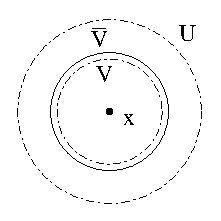
\includegraphics{./pic/T3alt.eps}
\item $\trax_4\eq \forall A$(abg)$\seq U$(offen)$\exists V$(offen)$: A\seq\ol{V}\seq U$\\
\includegraphics{./pic/T4alt.eps}
\item Es gibt auch $\trax_{3\durch{2}}$ und $\trax_5$\dots
\item Jeder \ul{metrische} Raum ist \ul{normal}, und jeder \ul{kompakte} Raum ist \ul{normal}
F"ur normale R"aume gelten wichtige S"atze "uber Existenz und Fortsetzbarkeit stetiger Funktionen.
\item {\sc L.A. Steen, J.A. Seebach} - Counterexamples in Topology (2nd ed. ,Springer 1978) | die Bibel f"ur pathologisch, veranlagte Topologen und Topologinnen.
\end{enumerate}
\end{bem}
\begin{beispiel}\label{3.18} zu Trennungsaxiome:
\begin{enumerate}
\item Die Klumpentopologie auf einer Menge mit mindestens zwei Elementen erf"ullt $\trax_1$.
\item Ein unendlicher Raum X mit kofiniter Topologie erf"ullt $\trax_1$ (die offene Umgebung $X\setminus \{ x\}$ trennt x von allen $y\in X$) aber nicht $\trax_2$ (da $U\cap V$ ist stets unendlich, da $(U\cap V)^c =U^c\cap V^c$ endlich ist).
\item Die {\sc Niemytzki}-Halbebene ist regul"ar aber nicht normal (ohne Beweis).
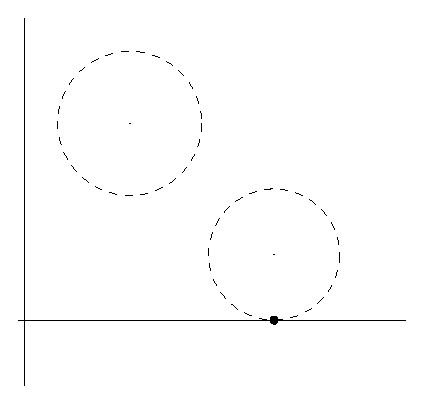
\includegraphics{./pic/niemytzkiright.eps}
\item Die Halbkugeltopologie\index{Halbkugeltopologie}\index{Topologie! Halbkugel-} auf der Halbebene ($\R\times[0,+\infty )$) mit Basisumgebungen:\\
$B_\eps(x)$ f"ur $x =(a,b)$ mit $0<\eps < b$\\
$C_\eps(x)$ f"ur $x =(a,0)$ mit $C_\eps(x):=\{ z\in \R\times\R_{>0}| 0<d(x,z)<\eps\}\cup\{ x\}$\\
\includegraphics{./pic/halfdisc.eps}\\
erf"ullt $\trax_2$ aber nicht $\trax_3$ (PS).
\end{enumerate}
\end{beispiel}
\newpage

\section{Continuity - Stetigkeit}
\subsection{Einleitung}
\begin{definition}\label{4.1}\index{Stetigkeit} von Stetigkeit\\
Seien ($X,\T_X$),($Y,\T_Y$) topologische R"aume, und $f:X\ra Y$:
$$f \mbox{ hei"st \ul{stetig}:}\eq \forall G\in\T_Y:\inv{f}(G)\in\T_X$$
d.h. $G$ offen in Y $\impl \inv{f}(G)$ offen in X\\
''$\inv{f}(\T_Y)\seq\T_X$''
\end{definition}
Daraus ergibt sich:\\
''f tut sich umso $\left\{\begin{array}{c}leichter\\schwerer\end{array}\right\}$, stetig zu sein,\\
je $\left\{\begin{array}{c}kleiner\\gr"o"ser\end{array}\right\}\T_Y$ und je $\left\{\begin{array}{c}gr"o"ser\\kleiner\end{array}\right\}\T_X$ ist; d.h.\\
je $\left\{\begin{array}{c}gr"ober\\feiner\end{array}\right\}\T_Y$ und je $\left\{\begin{array}{c}feiner\\gr"ober\end{array}\right\}\T_X$ ist.''\vspace*{1cm}\\
Alle identischen Funktionen $\mathbbm{1}_X = id_X:(X,\T )\ra (X,\T ), x\mapsto x$ sind stetig, denn G (offen) $\impl \inv{id}(G) = G$ offen.\\
Jede konstante Funktion $k_c:X\ra Y; x\mapsto c$ ist stetig, denn $\inv{k_c}(G) = \leer$ f"ur $c\notin G$ und $\inv{k_c}(G)=X$ f"ur $c\in G$.
\begin{satz}\label{4.2}{\sc Charakterisierung von Stetigkeit}\\
Seien $(X,\T_X$),($Y,\T_Y$) topologische R"aume, $A\seq X$, $B, C, G, S, U \seq Y$, $f:X\ra Y$. Dann sind die folgenden Aussagen "aquivalent:
\begin{enumerate}[(i)]
\item $f$ ist stetig, d.h. $G$ offen $\impl \inv{f}(G)$offen.
\item $\forall x\in X: U\in\umg{U}{f(x)}\impl\inv{f}(U)\in\umg{U}{x}$
\item $\forall x\in X:$ f"ur $\left\{\begin{array}{c}eine\\jede\end{array}\right\}$ Umgbas. $\umgbas{V}{f(x)}$ v. $f(x)$ gilt: $V\in\umgbas{V}{f(x)}\impl\inv{f}(V)\in\umg{U}{x}$.
\item F"ur alle $B$ aus $\left\{\begin{array}{c}einer\\jeder\end{array}\right\}$ Basis von $\T_Y$ gilt: $\inv{f}(B)$ offen in X.
\item F"ur alle $S$ aus $\left\{\begin{array}{c}einer\\jeder\end{array}\right\}$ Subbasis von $\T_Y$ gilt: $\inv{f}(S)$ offen in X.
\item $C$ abg. in Y$\impl \inv{f}(C)$ abg in X
\item $\forall A:f(\ol{A})\seq \ol{f(A)}$
\item[(vii)'] $\forall C: \ol{\inv{f}(C)}\seq\inv{f}(\ol{C})$
\end{enumerate}
{\bf Bemerkung:} zur Stetigkeit\\
''$f$ ist stetig in $x\in X$'' soll hei"sen: eine der Bedingungen (ii) oder (iii) (und damit beide) erf"ullt ist(sind) f"ur dieses betreffende x. Damit erhalten wir: $f$ stetig $\eq f$ stetig $\forall x\in X$.
\beweis{
\item[$(i)\impl (iv)_{jeder}$] klar, da jede Basis $\seq\T$.
\item[$(iv)_{jeder}\impl (iv)_{einer}$] klar.
\item[$(iv)_{einer}\impl (i)$] $\inv{f}(G)=\inv{f}(\bigcup_{i\in I}B_i)=\bigcup_{i\in I}\inv{f}(B_i)$ offen nach (O2).
\item[$(i)\impl (v)_{jeder}$] klar, da Subbasis $\seq\T$.
\item[$(v)_{jeder}\impl (v)_{einer}$] klar.
\item[$(v)_{einer}\impl (i)$]$\inv{f}(G)=\inv{f}(\bigcup_{i\in I}\bigcap_{j=1}^{n_i}S_{ij})=\bigcup_{i\in I}\bigcap_{j=1}^{n_i}\inv{f}(S_{ij})$ offen nach (O2),(O3).
\item[$(i)\impl (ii)$] Sei $U\in\umg{U}{f(x)}\implmit{\ref{2.7}}\exists V$(offen):$f(x)\in V\seq U; x\in\inv{f}(V)$offen\\
$\impl \inv{f}(V)\in\umg{U}{x}\impl\inv{f}(U)\in\umg{U}{x}$, da $\inv{f}(U)\supseteq\inv{f}(V).$
\item[$(ii)\impl (iii)_{jeder}$] klar, da $\umgbas{V}{f(x)}\seq\umg{U}{f(x)}$.
\item[$(iii)_{jeder}\impl (iii)_{einer}$] klar.
\item[$(iii)_{einer}\impl (i)$] Sei G (offen)$\seq Y, x\in\inv{f}(G)\impl f(x)\in G\in\umg{U}{f(x)}\\
\impl\exists V\in\umgbas{V}{f(x)}:f(x)\in V\seq G\impl\inv{f}(V)\seq\inv{f}(G)$.\\
nach (iii) ist $\inv{f}(V)\in\umg{U}{x}$, somit auch $\inv{f}(G)\in\umg{U}{x}\\
\impl\inv{f}(G)$ offen.
\item[$(i)\eq (vi)$]$\inv{f}(G)$ offen$\eq X\setminus\inv{f}(G)$abg$\eq \inv{f}(\underbrace{Y\setminus G}_{abg})$abg.
\item[$(vi)\impl (vii)$] $\inv{f}(\ol{f(A)})$abg $\supseteq \inv{f}(f(A))\supseteq A\implmit{\ref{2.34}(iv)} \inv{f}(\ol{f(A)})\supseteq\ol{A}\\
\impl f(\ol{A})\seq\ol{f(A)}$.
\item[$(vii)\impl (vii)'$] In (vii) ersetze A durch$\inv{f}(C):\\
f(\ol{\inv{f}(C)})\seq\ol{f(\inv{f}(C))}\seq\ol{C}\impl\ol{\inv{f}(C)}\seq\inv{f}(\ol{C})$
\item[$(vii)'\impl (vi)$]$C$ abg$\impl\inv{f}(C)=\inv{f}(\ol{C})\supseteq\ol{\inv{f}(C)}\supseteq\inv{f}(C)\implmit{\ref{2.35}(vi)}\inv{f}(C)$ abg.}
\end{satz}
Nun eine kleine Darstellung des obigen Beweises (nach dem Motto alle Wege f"uhren nach Rom).
$$\xymatrix{
&&(iii)_{jede}\ar[dr]\\
&(ii)\ar[ur]
&\smiley&(iii)_{eine}\ar[ddl]\\
(v)_{jede}\ar[d]
&&&&
(iv)_{jede}\ar[d]\\
(v)_{eine}\ar[rr]
&&(i)
	\ar[uul]
	\ar[ull]
	\ar[urr]
	\ar[d]
&&(iv)_{eine}\ar[ll]\\
&&(vi)
	\ar[u]
	\ar[dl]\\
&(vii)\ar[rr]
&&(vii)'\ar[ul]}$$

\begin{satz}\label{4.3}{\sc Zusammensetzung zweier stetiger Abbildungen}\\
Seien ($X,\T_X$), ($Y,\T_Y$), ($Z,\T_Z$) topologische R"aume und $f:X\ra Y$, $g:Y\ra Z$ stetige Abbildungen, dann ist auch $g\circ f:X\ra Z$ stetig.
\beweis{Sei G (offen)$\seq Z\impl \inv{(g\circ f)}(G)=\inv{g}(\underbrace{\inv{f}(G)}_{offen})$ offen.}
\end{satz}
Der folgende Satz bringt die angek"undigte Verallgemeinerung von Teil (iv) des Satzes \ref{2.53} - der Beweis geht v"ollig analog.
\begin{satz}\label{4.4}{\sc Stetigkeit via Netze}\\
Seien ($X,\T_X$), ($Y,\T_Y$) topologische R"aume und $f:X\ra Y$ eine Abbildung:\\
f ist genau dann stetig, wenn f"ur jedes Netz $(x_\lambda )_{\lambda\in\Lambda}$in X gilt:\\
$[(x_\lambda )_{\lambda\in\Lambda}\ra x]\impl [(f(x_\lambda ))_{\lambda\in\Lambda}\ra f(x)]$
\beweis{
\item[$(\impl)$]Sei $U\in\umg{U}{f(x)}\implmit{\ref{4.2}(ii)}\inv{f}(U)\in\umg{U}{x}\impl\exists\lambda_0\in\Lambda\forall\lambda\succeq\lambda_0:x_\lambda\in\inv{f}(U)\impl f(x_\lambda )\in U$.
\item[$(\lpmi)$] mit \ref{4.2}(ii); ind. Ann: $\exists x\in X:U\in\umg{U}{f(x)}:\inv{f}(U)$ {\sc keine} Umg. von $x\hfill (*)$\\
Sei $\umgbas{V}{x}$ Umgebungsbasis von x, (z.B. $\umgbas{V}{x}:=\umg{U}{x}$), $\Lambda :=\umgbas{V}{x}$ mit $\preceq :=\supseteq$.\\
$V\in\umgbas{V}{x}\implmit{(*)}V\not\seq\inv{f}(U)\impl\exists x_V\in V\setminus\inv{f}(U)$.\\
Wegen $x_V\in V$ gilt aber $x_V\ra x ($vgl $\ref{3.7}.3)$; aus der Voraussetzung erhalten wir $f(x_V)\ra f(x)$, ein Widerspruch $\wid$ zu $f(x_V)\notin U(\forall V)$.}
\end{satz}

F"ur den n"achsten Satz ben"otigen wir die Tatsache, dass eine Abbildung $f:X\ra\R^2$ bzw. $f:X\ra\C^2$ ($x\mapsto (f_1(x),f_2(x))$ von einem topologischen Raum nach $\R^2$ bzw. $\C^2$ genau dann stetig ist, wenn die beiden ''Komponentenfunktionen'' $f_1, f_2$ stetig sind. Die beiden Implikationsrichtungen ergeben sich aus den Beobachtungen:\\
\indent$(\impl )$ $\inv{f_1}(G_1) = \inv{f}(G_1\times\R ), \inv{f_2}(G_2) = \inv{f}(\R\times G_2 )$;\\
\indent$(\lpmi )$ $\inv{f}(G_1\times G_2)=\inv{f_1}(G_1)\cap\inv{f_2}(G_2)$\\
wobei $G_1$ und $G_2$ offene Teilmengen von $\R$ sind; "uberdies bilden die ''offenen Rechtecke'' $G_1\times G_2$ eine Basis der Topologie von $\R^2$, sodass \ref{4.2}(iv) anwendbar ist.\vspace*{0.3cm}\\
Das vorangegangene Argument funktioniert analog f"ur $f:X\ra\R^p$, $f:X\ra\C^q$; ja sogar f"ur $f:X\ra\prod_{j\in J}Y_j$ (wobei die $Y_j$ Topologische R"aume) $x\mapsto (f_j(x))_{j\in J}$. (PS)

\begin{satz}\label{4.5}{\sc Wichtiges "uber Stetigkeit}
\begin{enumerate}[(i)]
\item Sind $f,g:X\ramit{stetig}=\mathbb{K}$ ($\mathbb{K}\in\{\R ,\C\}$), dann sind $f\pm g$ und $f\cdot g$ stetig.
\item Ist $g:X\ra\mathbb{K}\setminus\{ 0\}$, dann gilt sogar: $\frac{f}{g}$ ist stetig.
\end{enumerate}
\beweis{Beispielhaft f"ur $f+g$:\\
Nach der Analysis-VO ist $\alpha :\R\times\R\ra\R ; (s,t)\mapsto s+t$ stetig. Au"serdem ist $h:X\ra X\times X; x\mapsto (f(x),g(x))$ stetig. Somit ist nach \ref{4.3} auch $\alpha\circ h$ stetig, und es gilt:\\
$(\alpha\circ h)(x)=\alpha (h(x))=\alpha (f(x),g(x))=f(x)+g(x)$.}
{\bf Bemerkung:} Genaugenommen muss man auf $\mathbb{K}\setminus\{ 0\}$ eigentlich die Spurtopologie (siehe Kapitel V) betrachten. Wir k"onnen aber $\mathbb{K}\setminus\{ 0\}$ einfach als metrischen Raum\footnote{nach PS ist es egal welche (von einer Norm induzierten) Metrik wir w"ahlen, z.B. die euklidische Metrik} betrachten (und somit auch als topologischen Raum)\\
Aus der Stetigkeit von $|\_ |: \mathbb{K}\ra\R ;x\mapsto |x|$ folgt mittels Satz \ref{4.3}, dass weiters $| f |, \max\{ f,g\} :=\durch{2} (f+g+|f-g|), \min\{ f,g\} := \durch{2}(f+g-|f-g|)$ stetig sind.
\end{satz}
Der Satz \ref{4.5}(i) gilt sinngem"a"s auch f"ur normierte R"aume bzw. Algebren.
\begin{definition}\label{4.6}{Hom"oomorphismus}\index{Hom{\"o}omorphismus}
Seien X, Y topologische R"aume, $f:X\ra Y$
\begin{enumerate}[(i)]
\item f hei"st \ul{Hom"oomorphismus} zwischen $(X,\T_X)$ und $(Y,\T_Y):\eq$ f ist stetig \& bijektiv und $\inv{f}$ auch stetig.
\item X und Y sind \ul{hom"oomorph} zu einander ($X\cong Y$) :$\eq \exists f$ (Hom"oomorphismus): $X\ra Y$
\end{enumerate}
Ein Hom"oomorphismus ist also ein topologischer Isomorphismus; Hom"oomorphie ist also eine "Aquivalenzrelation auf topologischen R"aumen:\\
$X\cong X$ via $id_X$\\
$X\stackrel{f}{\cong}Y\impl Y\stackrel{\inv{f}}{\cong}X$\\
$X\stackrel{f}{\cong}Y \et Y\stackrel{g}{\cong}Z\impl X\stackrel{g\circ f}{\cong}Z$
\end{definition}
Offenbar gilt f"ur $A\seq X$, $f:X\ramit{Hom"o.}Y$\\
$A$ offen[abg]$\eq f(A)$ offen[abg] ($A=\hspace*{-0.8cm}\underbrace{\inv{(\inv{f})}}_{\mbox{inverses Urbild}}\hspace*{-0.7cm}(A))$\vspace*{-0.5cm}\\
$A\in\umg{U}{x}\eqmit{\ref{4.2}(ii)}f(A)\in\umg{U}{f(x)}$\vspace*{0.5cm}\\
Hom"omorphe R"aume sind vom Standpunkt der Topologie nicht unterscheidbar.\vspace*{0.5cm}\\
Eine Eigenschaft (topologischer R"aume) hei"st \ul{topologische Eigenschaft}\index{topologische Eigenschaft}, wenn sie mit X auch jeder zu X hom"oomorphe Raum Y besitzt. Beispiele f"ur topologische Eigenschaften sind:\\
\hspace*{2cm}Metrisierbarkeit\\
\hspace*{2cm}Separabilit"at\\
\hspace*{2cm}AA1\\
\hspace*{2cm}AA2\\
\hspace*{2cm}Kompaktheit (Kapitel VI)\\
\hspace*{2cm}Zusammenhang (Kapitel VII)\\
(Zum Beweis transportiert man einfach die relevanten Objekte | i.e. Metriken, abzb. dichte Teilmengen, (Umgebungs-) Basen etc. mittels f von X nach Y.)\\
Beispiele f"ur nicht-topologische Eigenschaften sind etwa solche, die gewisse Eigenschaften einer die Topologie betreffenden Metrik [Norm] miteinbeziehen, wie etwa:
\begin{description}
\item ''X ist auch vollst"andig als metrischer Raum''
\item ''X ist auch ein beschr"ankter metrischer Raum''
\end{description}
z.B. $f:\R^+\ra\R^+ ; x\mapsto \frac{x}{x+1}$ ist Hom"oomorphismus: $X:= \R^+$ ist vollst"andiger metrischer Raum bez"uglich einer unbeschr"ankten Metrik; $f(X) =[0,1)$ hingegen ist nicht vollst"andig f"ur $d(x,y)\leq1$
\newpage
\subsection{Lemma von {\sc Urysohn}}
F"ur disjunkte abgeschlossene Intervalle (in $\R$) $A=[a,b]$ und $B=[c,d]$ ist es leicht eine stetige Funktion anzugeben mit $f:\R\ra\R$ und $0\leq f\leq 1$, $f|_A =0$ und $f|_B=1$:\\
\hspace*{4.5cm}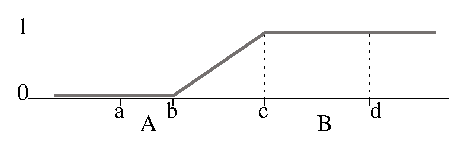
\includegraphics{./pic/uryreal.eps}\\
Der folgende wichtige Satz zeigt, dass sich eine derartige stetige Funktion sogar allgemein in normalen topologischen R"aumen und zu disjunkten abgeschlossenen Mengen konstruieren l"asst.

\begin{satz}\label{4.7}{\sc Lemma von Urysohn}\\
Ein topologischer Raum X erf"ullt genau dann das Trennungsaxiom $\trax_4$, wenn gilt:
$$\forall A,B\mbox{(beide abg.)}\seq X, A\cap B=\leer, \exists f;X\ra [0,1]: f\mbox{stetig}, f|_A=0, f|_B=1$$
\beweis{
\item[($\impl$)] Ist f wie oben, dann trennen $U:=\{x\in X|f(x)<\durch{2}\}$ und $V:=\{x\in X|f(x)>\durch{2}\}$ die beiden Mengen $A, B$ offen $\impl \trax_4$
\item[($\lpmi$)] Setze $G:=B^c$, dann gilt $A$(abg.)$\seq G_1$(offen);\\
$\implmit{\ref{3.17}(iv)}\exists G_\durch{2}$(offen):$A\stackrel{(\star )}{\seq} G_\durch{2}\seq\ol{G_\durch{2}}\stackrel{(\star\star )}{\seq} G_1$\\
Bei $(\star )$ und $(\star\star )$ k"onnen wir wiederum $\trax_4$ anwenden und erhalten $G_\durch{4}$ und $G_\frac{3}{4}$ mit:
\hspace*{1cm}$A\seq G_\durch{4}\seq \ol{G_\durch{4}}\seq G_\durch{2}\seq \ol{G_\durch{2}}\seq G_\frac{3}{4}\seq \ol{G_\frac{3}{4}}\seq G_1$\vspace*{0.2cm}\\
Induktiv definieren wir so f"ur jede ''dyadisch, rationale Zahl''\\
$r\in D:=\{\frac{k}{2^n} (\in\Q)|n,k\in\N, 0<k<n\}$ eine offene Menge $G_r$, sodass gilt:\\
$A\seq G_r\seq\ol{G_r}\seq G_1$ und $\ol{G_{r_1}}\seq G_{r_2}$f"ur $r_1<r_2$\\
Nun zu unserer Funktion $f:X\ra [0,1]$
$$x\mapsto\left\{\begin{array}{l r} 1&x\notin \bigcup_{r\in D}G_r \\ \inf\{ r\in D|x\in G_r\} &\mbox{sonst}\end{array}\right.$$
$\bullet$ $x\in A \impl\forall r\in D: x\in G_r\impl f(x)=0$\\
$\bullet$ $x\in B \impl x\notin G_1\impl\forall r\in D: x\notin G_r\impl x\notin\bigcup_{r\in D}G_r\impl f(x)=1$\\
$\bullet$ \ul{f ist stetig (bei jedem $x\in X$)}\\
Wir zeigen zun"achst:($r\in D$)\vspace*{-0.1cm}\\
$$\{x\in X|f(x)<r\}\stackrel{(\star )}{\seq}G_r\stackrel{\mbox{klar}}{\seq}\ol{G_r}\stackrel{(\star\star )}{\seq}\{ x\in X|f(x)\leq r\}$$
ad($\star$) $f(x)<r\impl\exists s<r :x\in G_s\impl x\in G_r$\\
ad($\star\star$) $x\in\ol{G_r}\impl \forall s\geq r :x\in G_s\impl\forall s\geq r :f(x)\leq s\impl f(x)\leq r$\\
$0<f(x)<1$ [wollen nun f in Umgebung von x in vorgegebenes $B_\eps (f(x))=(f(x)-\eps , f(x)+\eps )$ reinbringen.]\\
Sei $\eps>0 \impl \exists r,s\in D:\quad f(x)-\eps <r<f(x)<s<f(x)+\eps\\
\impl U:=G_s\setminus \ol{G_r}$ ist \\
$\framebox{offene}^\alpha$ $\framebox{Umgebung von x}^\beta$mit $\framebox{$f|_U \in (f(x)-\eps ,f(x)+\eps )$}^\gamma$\\
$\alpha )$ $U=G_s\setminus\ol{G_r} =G_s\cap (\ol{G_r})^c$offen\\
$\beta )$ $\left.\begin{array}{r}f(x)<s\implmit{(\star )} x\in G_s\\ f(x)>r\implmit{(\star\star )} x\notin G_r\end{array}\right\}\impl x\in U$\vspace*{0.7cm}\\
$\gamma )$ \vspace*{-1.1cm}\\
\hspace*{0.5cm}$\xymatrix@R=-0.3cm{&y\in G_s\implmit{(\star\star )}f(y)\leq s\\
y\in U\ar@{=>}[ur]\ar@<-0.1cm>@{=>}[dr]\\
&y\notin\ol{G_r}\implmit{(\star )} f(y)\geq r }$\vspace*{-1.4cm}\\
\hspace*{6.4cm}$\Bigg\}\impl f(y)\in [r,s]\seq (f(x)-\eps, f(x)+\eps )$\vspace*{0.15cm}\\
$\ul{f(x)=0}:$ F"ur $s\in (0,\eps)\cap D$ nimmt f auf $U:=G_s$ nur Werte in $[0,s)\seq[0,\eps )$ an; U ist offene Umgebung von x (Beweis wie oben $\alpha ), \beta )$ oben )\\
$\ul{f(x)=1}:$ F"ur $r\in (1-\eps ,1)\cap D$ nimmt f auf $U:=X\setminus\ol{G_r}$ nur Werte in $[r,1]\seq (1-\eps,1]$ an; U ist offene Umgebung von x (Beweis wie oben $\alpha ), \beta )$ oben )}
\end{satz}
Skizze zum Beweis von \ref{4.7}:\vspace*{2cm}\\
\hspace*{-1cm}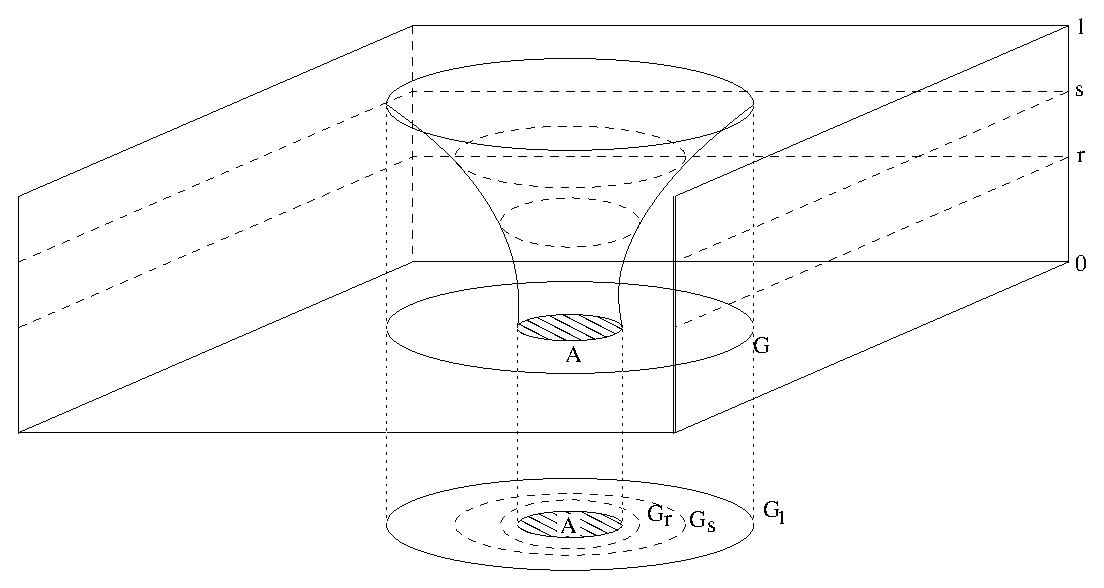
\includegraphics[scale=0.9]{./pic/urysohn.eps}
\newpage
\section{Spurtopologie, initiale und finale Topologie}
Grunds"atzlich handelt dieses Kapitel davon neue Topologien aus bereits vorhandenen Topologien zu ''basteln'', im speziellen Topologien auf Teilmengen Y eines topologischen Raumes ($X,\T$) (die Spurtopologie auf Y) bzw. per Transport entlang von Abbildungen - gegen (initiale Topologie) und in die Pfeilrichtung (finale Topologie). Die Spurtopologie wird sich letztendlich als Spezialfall der initialen Topologie herausstellen.
\subsection{Spurtopologie}
\begin{definition}\label{5.1}Spurtopologie\index{Spurtopologie}\\
Sei ($X,\T$) ein topologischer Raum und $Y\seq X$dann ist:
$$\T |_Y :=\T\cap Y:=\{ G\cap Y| G\in\T\}\mbox{\dots die \ul{Spurtopologie} (auf Y bez"uglich $\T$)}$$
oder die von $\T$ auf Y induzierte Topologie.\\
$\T |_Y$ erf"ullt tats"achlich (O1)-(O3): $\leer =\leer\cap Y$, $Y=X\cap Y$\vspace*{0.1cm}\\
\hspace*{6.2cm}$\bigcup_{j\in J}(G_j\cap Y)= (\bigcup_{j\in J}G_j)\cap Y$\vspace*{0.2cm}\\
\hspace*{6.2cm}$\bigcap_{j=1}^n(G_j\cap Y)= (\bigcap_{j=1}^nG_j)\cap Y$\\
\end{definition}

\begin{prop}\label{5.2} Sei ($X,\T$) ein topolog. Raum $Y\seq X; \framebox{$\T_Y:=\T |_Y$}\\
x\in Y, (x_\lambda)_{\lambda\in\Lambda}$ ein Netz in Y; $A, U\seq Y, B,W \seq X;\\
\umg{U}{x}^Y[\umg{U}{x}]$ ein Umgebungssystem von x bez"uglich $\T_Y [\T ]$;\\
$\ol{A}^Y [\ol{A}^X ]$ der Abschluss von A bez"uglich $\T_Y$(in Y) [$\T$ (in X)].\\
Dann gilt:
\begin{enumerate}[(i)]
\item $U\in\umg{U}{x}^Y\eq\exists W\in\umg{U}{x}: U=W\cap Y$
\item A abg. bez. $\T_Y$ (''A abg. in Y'')$\eq \exists B$ (abg. bez. $\T ): A=B\cap Y$
\item $\ol{A}^Y=\ol{A}^X\cap Y$
\item $((x_\lambda )_{\lambda\in\Lambda}\ra x$) bez. $\T_Y\eq (x_\lambda\ra x)$ bez $\T$
\item Sei f (stetig): $(X,\T )\ra (\widetilde{X},\widetilde{\T})$. Dann ist $f|_Y$(stetig):$(Y,\T_Y )\ra (\widetilde{X},\widetilde{\T})$
\end{enumerate}
\beweis{
\item[(i) ($\impl$)] Sei $U\in\umg{U}{x}^Y\implmit{\ref{2.7}}\exists V\in\T_Y :x\in V\seq U; V=G\cap Y, G\in\T$\\
\hspace*{4cm}$x\in V:\impl x\in G\impl G\in\umg{U}{x}$\\
\hspace*{4cm}$\implmit{(U2)} W:=G\cup U\in\umg{U}{x}$\\
\hspace*{2.6cm}$W\cap Y= (G\cup U)\cap Y= (G\cap Y)\cup (U\cap Y) = V\cup U = U$
\item[($\lpmi$)] $W\in\umg{U}{x}\implmit{\ref{2.7}}\exists G\in\T :x\in G\seq W$\\
\hspace*{1.6cm}$\impl x\in \underbrace{G\cap Y}_{\in\T_Y} \seq \underbrace{W\cap Y}_{U:=}$\\
\hspace*{1.6cm}$\implmit{\ref{2.6}}G\cap Y\in\umg{U}{x}^Y\implmit{(U2)}U\in\umg{U}{x}^Y$.
\item[(ii)] A $\T_Y$-abg $\eq Y\setminus A\in\T_Y\\
\hspace*{1.55cm}\eq\exists G\in\T :Y\setminus A=G\cap Y\\
\hspace*{1.55cm}\eq\exists G\in\T A= (X\setminus G)\cap Y\\
\hspace*{1.2cm}\eqmit{X\setminus G=B}\exists B(\T -$abg $):A=B\cap Y$\vspace*{-3cm}\\
\hspace*{8cm}\includegraphics[scale=1.5]{./pic/5.2ii.eps}
\item[(iii)]Wir zeigen: $\ol{A}^X$ ist die kleinste $\T_Y$-abg Menge die A enth"alt, nach \ref{2.34}(iv) somit gleich $\ol{A}^Y:\\
\bullet \ol{A}^X\cap Y$ ist $\T_Y$-abg nach (ii)\\
$\bullet\ol{A}^X\cap Y\seq A\cap Y=A\\
\bullet$ Sei C ($\seq Y$) $\T_Y$-abg mit $C\supseteq A$\\
\hspace*{0.4cm}$\implmit{(ii)}C=B\cap Y, B\T$-abg $\impl A\seq C\seq B\impl\ol{A}^X\seq B$\\
\hspace*{0.4cm}$\impl\ol{A}^X\cap Y\seq B\cap Y=C$\\
\hspace*{0.4cm}$\impl\ol{A}^X\cap Y$ ist minimal mit $''\supseteq A$ \& ist $\T_Y$-abg''.
\item[(iv)] ($x_\lambda\ra x$) bez. $\T\eq\forall U\in\umg{U}{x}:\exists\lambda_0\in\Lambda :\forall\lambda\succeq\lambda_0:\mbox{$x_\lambda\in U\eqmit{(x_\lambda\in Y !)}x_\lambda\in U\cap Y=V$}$\\
\hspace*{2.95cm}$\eqmit{(i)}\forall V\in\umg{U}{x}^Y:\exists\lambda_o\in\Lambda :\forall\lambda\succeq\lambda_0:x_\lambda\in V\\
\hspace*{2.8cm}\eq x_\lambda\ra x$ bez. $\T_Y$.
\item[(v)] Sei H offen in ($\widetilde{X},\widetilde{\T}$), dann ist:$\inv{(f|_Y)}(H)=\{x\in Y|f(x)\in H\}=\underbrace{\inv{f}(H)}_{\in\T}\cap Y$\vspace*{-0.5cm}\\
offen bez. $\T_Y$, $f$ also stetig.}\vspace*{-0.3cm}
\end{prop}
\begin{beispiel}\label{5.3} zur Spurtopologie
\begin{enumerate}
\item $X=\R$ mit euklid. Topologie, $Y=[0,1)$ mit Spurtopologie:\\
$A_1=[0,\durch{2})\quad$ offen in Y, {\sc nicht} offen in $\R$ [$A_1=Y\cap(-1,\durch{2})$!]\\
$A_2=(\durch{2},1)\quad$ offen in Y, offen in $\R$\\
$A_3=[0,\durch{2}]\quad$ abg in Y, abg in $\R$\\
$A_4=[\durch{2},1)\quad$ abg in Y, {\sc nicht} abg in $\R$ [$A_4=Y\cap[\durch{2},2]$!]
\item ($\R,\T_{eukl}$), $Y=\Z$ mit Spurtopologie (analog f"ur $\N$)\\
Die Spurtopologie auf $\Z$ ist die diskrete Topologie, denn $\{ k\}=\Z \cap \underbrace{(k-\durch{2},k=\durch{2})}_{\mbox{offen in $\R$}}$\vspace*{-0.7cm}\\ f"ur jedes $k\in\Z$
\item $(\R ,\T_{eukl})$, $Y=\{ 0\}\cup \{\durch{n}|n\in\N\}$\\
In der Spurtopologie ist jedes ''$\durch{n}$'' offen, denn $\{\durch{n}\} = Y\cap (\durch{n+1},\durch{n-1})$,\\
(mit $\durch{0}:=\infty$), aber eine Umgebungsbasis von 0 in Y ist z.B. gegeben durch die Mengen $V_k:=\{0, \durch{k}, \durch{k+1}, \durch{k+2}, \dots\} = Y\cap B_\durch{k-1}(0)$.
\item ($\R^2,\T_{eukl})$, $Y=\mathbb{D}^1:=\{x\in\R^2|\norm{x}_2<1\};\\
M:=\{ x=(x_1,x_2)\in\mathbb{D}^1|x_2\geq 0\}$ abg in $\mathbb{D}^1$ da:\\
$M=\mathbb{D}^1\cap\{x=(x_1,x_2)\in\R^2|${\scriptsize$\left.\begin{array}{c}-2\leq x_1\leq +2\\0\leq x_2\leq +2\end{array}\right.$}$\}$\\
aber M ist nicht abgeschlossen in $\R^2$.\\
\vspace*{-3cm}\\
\hspace*{7cm}\includegraphics{./pic/5.3.4.eps}\vspace*{-2.5cm}\\
\end{enumerate}
\end{beispiel}
\subsection{Fortsetzungssatz von {\sc Tieze-Urysohn}}
\begin{satz}\label{5.4}{\sc Fortsetzungssatz von Tieze-Urysohn}\\
Sei ($X,\T$) ein topologischer $\trax_4$ Raum; weiters $A$(abg.) $\seq X$ und $f:A\ramit{stetig} [-a,+a]$, bez"uglich $\T|_A$\\
Dann existiert eine stetige Funktion $F:X\ra [-a,+a]$, die $f$ fortsetzt (d.h. $F|_A =f$).
\beweis{Technischer Kernpunkt des Beweises ist die folgende Konstruktion:
\item[\ul{Behauptung}] Ist $g:A\ra [-c,+c]$ stetig, dann existiert eine stetige Funktion; $h:X\ra [-\frac{c}{3},+\frac{c}{3}]$ mit $|g-h|\leq\frac{2c}{3}$ auf A.
\beweis{Sei $B_+:=\{x\in A|g(x)\in[\frac{c}{3},c]\}, B_-:=\{x\in A|g(x)\in[-c,-\frac{c}{3}\}$\\
Dann sind $B_+,B_-$abgeschlossen in A(somit in X) und disjunkt.\\
Satz \ref{4.7} liefert eine stetige Funktion:\\
$\widetilde{h}:X\ra[0,1]$ mit $\widetilde{h}|_{B_+}=1, \widetilde{h}|_{B_-}=0$\\
(falls $B_+=\leer \ra \widetilde{h}=0$ [$B_1=\leer \ra \widetilde{h}=1$]).\\
$h(x):= \frac{2c}{3}(\widetilde{h}(x)-\durch{2})$ leistet das Gew"unschte:\\
h ist stetig, $|h|\leq\frac{2c}{3}\cdot\durch{2}=\frac{c}{3}$ und $|g-h|\leq\frac{2c}{3}$ auf A:\\
$x\in B_+\impl \widetilde{h}(x)=1\impl h(x)=\frac{c}{3}\impl g(x)-h(x)\in [0,\frac{2c}{3}]$\\
$x\in B_-\impl \widetilde{h}(x)=0\impl h(x)=-\frac{c}{3}\impl g(x)-h(x)\in [-\frac{2c}{3},0]$\\
$x\in A\setminus(B_+\cup B_-)\impl g(x)\in (-\frac{c}{3},+\frac{c}{3})\impl |g(x)-h(x)|\leq |f(x)|+|g(x)|\leq\frac{c}{3} +\frac{c}{3}=\frac{2c}{3}$
	}
Wir wenden nun obige Konstruktion auf $f$ an (mit $c = a$), und erhalten eine stetige Funktion $f_1:X\ra[-\frac{a}{3},+\frac{a}{3}]$ mit $|f-f_1|\leq\frac{2a}{3}$ auf A.\\
Wir wenden nun obige Konstruktion auf $f-f_1|_A$ an (mit $c =\frac{2a}{3}$), und erhalten eine stetige Funktion $f_2:X\ra[-\frac{2a}{9},+\frac{2a}{9}]$ mit $|f-f_1-f_2|\leq\frac{4a}{9}$ auf A.\\
Per Induktion erhalten wir so eine Folge $f_1,f_2\dots$ von Funktionen auf X mit den Eigenschaften:
$$|f_n|\leq\frac{a}{3}(\frac{2}{3})^{n-1}$$
$$f-(\sum_{j=1}^n f_j)|\leq a(\frac{2}{3})^n$$
Die Reihe $\sum_{j=1}^\infty f_j$ konvergiert gleichm"a"sig auf X gegen eine Funktion $F(x)$. Diese ist als Grenzwert stetiger Funktionen wiederum stetig [Analysis-VO!] \\
F"ur F gilt:\\
$|F(x)|\leq\sum_{j=1}^\infty |f_j(x)|\leq\frac{a}{3}\sum_{j=1}^\infty (\frac{2}{3})^{j-1}=\frac{a}{3}\durch{1-\frac{2}{3}}=a$\\
$x\in A\impl f(x)-F(x)=\lim_{n\ra\infty} f(x)-(\sum_{j=1}^n f_j)=0\impl f(x)=F(x)$\\
F leistet somit das gew"unschte.}
\end{satz}
\subsection{Initiale- und finale Topologie}
\setcounter{definition}{5}
{\bf V.5.a }\label{5.5.a}{\sc Transport von Topologien entlang einer Abbildung}\vspace*{0.4cm}\\
\begin{minipage}{7cm}
$f:\stackrel{\mbox{\scriptsize Menge}}{X}\ra \stackrel{\mbox{\scriptsize top. Raum}}{(Y,\T_Y)}$\\
will auf X (am Pfeil\ul{beginn} )eine\\
''interessante'' Topologie $\T_X$ definieren,\\
sodass f stetig bez"uglich $\T_X,\T_Y$ wird.\\
\ul{initiale Topologie $\T_X$}
\end{minipage}\hspace*{0.5cm}
\begin{minipage}{7cm}
$f:\stackrel{\mbox{\scriptsize top. Raum}}{(X,\T_X}\ra \stackrel{\mbox{\scriptsize Menge}}{Y}$
will auf Y (am Pfeil\ul{ende} )eine ''interessante'' Topologie $\T_Y$ definieren, sodass f stetig bez"uglich $\T_X,\T_Y$ wird.\\
\ul{finale Topologie $\T_Y$}
\end{minipage}
Stetigkeit von $f:(X,\T_X)\ra(Y,\T_Y):$\\
\hspace*{5cm}$f \mbox{ stetig }\eq\inv{f}(\T_Y)\seq\T_X$\\
\hspace*{6cm}\includegraphics[scale=0.8]{./pic/5.5.eps}\\
\begin{minipage}[l]{7.2cm}
$\T_Y$ gegeben$\impl\T_X$ muss mindestens so gro"s sein, dass es $\inv{f}(\T_Y)$ enth"alt.\vspace*{0.3cm}\\
$\T_X$ maximal:$\T_X = 2^X$ (diskret) - ok aber uninteressant.\vspace*{0.3cm}\\
$\T_X$ minimal:\\
$\T_X =\inv{f}(\T_Y)$ d.h.\\
\framebox{$G\in\T_X:\eq\exists H\in\T_Y: G=\inv{f}(H)$}\\
Die \ul{initiale Topologie} auf X\index{initiale Topologie}\index{Topologie!initiale} bez"uglich $f:X\ra(Y,\T_Y)$ ist gegeben durch:\vspace*{-0.3cm}\\
$$\T_X:=\{\inv{f}(G)|G\in\T_Y\}$$
Sie ist die gr"obste Topologie auf X, sodass f stetig ist.\vspace*{0.3cm}\\
{\bf (O1)}$\leer =\inv{f}(\leer )$ offen\\
$X=\inv{f}(Y)$ offen\\
{\bf (O2)}\vspace*{-0.7cm}\\
{\small $\bigcup_{i\in I}G_i=\bigcup_{i\in I}\inv{f}(H_i)=\inv{f}(\overbrace{\bigcup_{i\in I} H_i)}^{\mbox{offen}}$ off.}\\
{\bf (O3)}\vspace*{-0.1cm}\\
{\small $\bigcap_{i=1}^nG_i=\bigcap_{i=1}^n\inv{f}(H_i)=\inv{f}(\underbrace{\bigcap_{i=1}^n H_i}_{\mbox{offen}})$ off.}
\end{minipage}\hspace*{0.5cm}
\begin{minipage}[l]{7cm}
$\T_X$ gegeben$\impl\T_Y$ darf h"ochstens so gro"s sein, dass $\inv{f}(\T_Y)$ in $\T_X$ enthalten ist.\vspace*{0.3cm}\\
$\T_Y$ minimal:$\T_Y=\{\leer ,Y\}$ (Klumpen) - ok aber uninteressant.\vspace*{0.3cm}\\
$\T_X$ maximal:\\
$\inv{f}(\T_Y) = \T_X$ d.h.\\
\framebox{$H\in\T_Y:\eq\exists \inv{f}(H)\in\T_X$}\\
Die \ul{finale Topologie} auf X\index{finale Topologie}\index{Topologie!finale} bez"uglich $f:(X,\T_X)\ra Y$ ist gegeben durch:\vspace*{-0.3cm}\\
$$\T_Y:=\{H\seq Y|\inv{f}(H)\in\T_X\}$$
Sie ist die feinste Topologie auf Y, sodass f stetig ist.\vspace*{0.3cm}\\
{\bf (O1)}$\inv{f}(\leer_Y )=\leer_X\impl \leer_Y$ offen\\
$\inv{f}(Y)= X\impl Y$ offen\\
{\bf (O2)}{\small $H_i$ alle offen, d.h. alle$\inv{f}(H_i)\in\T_X$\\
$\impl \inv{f}(\bigcup_{i\in I}H_i)=\bigcup_{i\in I}\inv{f}(H_i)\in\T_X\impl$\\
\hspace*{5.5cm}$H_i$ offen}\\
{\bf (O3)}\\
{\small $H_1... H_n$ alle offen, d.h. alle $\inv{f}(H_i)\in\T_X\\
\impl\inv{f}(\bigcap_{i=1}^nH_i)=\bigcap_{i=1}^n\inv{f}(H_i)\in\T_X\impl$\\
\hspace*{5.5cm}$H_i$ offen}
\end{minipage}
\newpage
Wir bringe je eine wichtige Anwendung der Konstruktion von initialen und finalen Topologien entlang einer Abbildung.\vspace*{1cm}\\
\begin{minipage}[l]{7cm}
\ul{initiale Topologie} bez"uglich\\
$\iota:Y\ra (X,\T_X); Y\seq X$ und $\iota (y)=y$ die \ul{Einbettungsabbildung von Y in X} ist.\footnote{Achtung! hier sind die Rollen von X und Y gegen"uber oben vertauscht !} Es gilt f"ur jedes $A\seq X:\\
\inv{\iota}(A)=A\cap Y$, denn $x\in \inv{\iota}(A)\eq\\
x\in Y\et \iota (x)[=x]\in A\eq x\in A\cap Y$\\
Veranschaulichung:\\
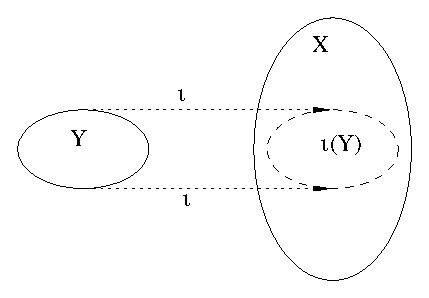
\includegraphics{./pic/einbettung.eps}\\
Nach Def der initialen Topologie $\T_Y$ ist:\\
{\footnotesize $\T_Y:=\{\inv{\iota}(H)|H\in\T_X\}=\{H\cap Y|H\in\T_X\}$}
$\impl\T_Y$ ist die Spurtopologie\index{Spurtopologie}, sie ist somit die gr"obste sodass $\iota$ stetig ist.
\end{minipage}\hspace*{0.5cm}
\begin{minipage}[l]{7.4cm}
\ul{finale Topologie} bez. p$:(X,\T_X)\ra Y$,\\
Y$:=\hspace*{-0.1cm}\{K|\hspace*{-0.2cm}\left.\begin{array}{l}\mbox{\scriptsize K "Aquivalenzklasse bez. fixer}\\\mbox{\scriptsize "Aquivalenzrelation $\sim$ auf X}\end{array}\right.\hspace*{-0.2cm}\}\hspace*{-0.15cm}=\hspace*{-0.1cm}X/\hspace*{-0.1cm}_\sim$ und p$(x)=K$, wobei $x\in K$; p hei"st \ul{kanonische Projektion von X auf $X/\hspace*{-0.1cm}_\sim$}
Veranschaulichung\\
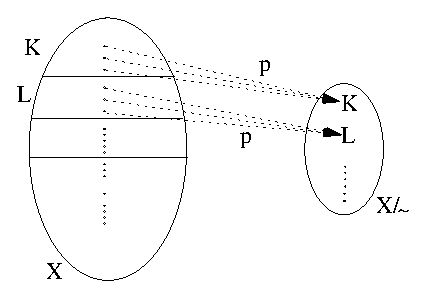
\includegraphics{./pic/projection.eps}\\
$\T_Y=\{ H\seq X/_\sim |\inv{\mbox{p}}(H)\in\T_X\}$ \ul{Quotiententopologie bez. $\T_X$ auf $X/_\sim$}\\
Beispiel: V VR, W TR von V, $v_1\sim v_2 :\eq v_1-v_2\in W, V/_\sim = V/_W$\vspace*{1.7cm}
\end{minipage}\vspace*{0.1cm}\\
\newpage
{\bf V.5.b }\label{5.5.b}{\sc Transport von Topologien entlang mehrerer Abbildungen}\vspace*{0.4cm}\\
\begin{minipage}{7cm}
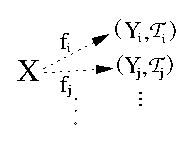
\includegraphics{./pic/initmehr.eps}\\
Gesucht als \ul{initiale Topologie}: Gr"obste Topologie $\T_X$ auf X sodass alle $f_i$ stetig sind, d.h. $\inv{f_i}(\T_i)\seq\T_X\quad \forall i\in I\\
\impl\T_X$ minimal, sodass gilt:
$$\T_X\supseteq\hspace*{-0.8cm} \underbrace{\bigcap_{i\in I}\inv{f_i}(\T_i)}_{\mbox{\scriptsize erf"ullt i.A. nicht (O1)-(O3)}}$$
Daher ernennt man $\Sb :=\bigcap_{i\in I}\inv{f_i}(\T_i)$ zur Subbasis von $\T_X$\\
Also:\\{\small
Die $\inv{f_i}(H_i), (H_i\in\T_i)$ bilden Sb f"ur $\T_X$\\
Die $\inv{f_{i_1}}(H_{i_1})\cap\dots\cap\inv{f_{i_n}}(H_{i_n})$ bilden eine Basis f"ur $\T_X$\\
Die bel. Vereinigungen solcher endl. Durchschnitte bilden die offenen Mengen von $\T_X$}
\end{minipage}\hspace*{0.5cm}
\begin{minipage}{7cm}
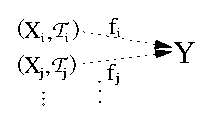
\includegraphics{./pic/finamehr.eps}\\
Gesucht als \ul{finale Topologie}: Feinste Topologie $\T_Y$ auf Y, sodass alle $f_i$ stetig sind, d.h. $\inv{f_i}(\T_Y)\seq\T_i\quad\forall i\in I$\\
$\T_Y:=\{ H\seq Y|\forall i\in I:\inv{f_i}(H)\in\T_i\}$\\
erf"ullt (O1)-(O3) (Beweis analog zu V.5.a)\vspace*{4.8cm}\\
\end{minipage}

\begin{beispiel}\label{5.6}zu intialer Topologie entlang mehrerer Abbildungen\\
Seien $(X_i,\T_i)$, ($\forall i\in I$) Topologische R"aume, Sei $X=\prod_{i\in I}X_i$. F"ur $k\in I$(bel, fix) sei die ''\ul{k-te Projektionsabbildung}'' $\pr_k: X\ra X_k; (x_i)_{i\in I}\mapsto x_k$\vspace*{1cm}\\
vgl. $\pr_1:\R^2\ra\R ,(x_1,x_2)\mapsto x_1$\\
$\pr_2:\R^2\ra\R ,(x_1,x_2)\mapsto x_2$\vspace*{-2cm}\\
\hspace*{5.5cm}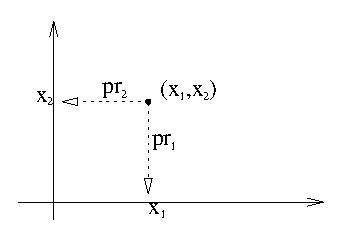
\includegraphics[scale=0.7]{./pic/pr.eps}\\
\includegraphics{./pic/projektionsabb.eps}\\
Was ist die initiale Topologie $\T_X$ auf X bez"uglich der $\pr_k$ $(k\in I)$? Das ist die gr"obste Topologie, sodass alle $\pr_k$ stetig sind (die feinste derartige ist die diskrete Topologie - fad!); $\T_X$ hat als Subbasis gerade die $\inv{\pr_k}(H_k), (H_k\in\T_k)$\\
Nun gilt:\\
\hspace*{2cm}$\inv{\pr_k}(H_k)=\{x=(x_i)_{i\in I}|\pr_k(x)\in H_k\}\\
\hspace*{3.6cm}=\{x=(x_i)_{i\in I}|x_k\in H_k\}\\
\hspace*{3.6cm}=\prod_{i\in I\setminus\{k\}}X_i\times H_k$\\
diese Subbasis ist genau die der \ul{Produkttopologie} siehe \ref{2.23}.1; diese ist somit die gr"obste sodass alle Projektionen stetig sind.
\end{beispiel} 
\begin{prop}\label{5.7}{Produkttopologie $\eq$ koordinatenweise Konvergenz}\\
Sei $X=\prod_{i\in I}X_i$ mit $\T_{prod}$ dann gilt:
$$(x_\lambda )_{\lambda\in\Lambda}\ra x\in (X,\T_{prod})\eq\forall k\in I (\pr_k(x_\lambda ))_{\lambda\in\Lambda}\ra \pr_k(x)$$
\beweis{
\item[($\impl$)] $\pr_k$ sind stetig nach \ref{5.6}; wende \ref{4.4} an.
\item[($\lpmi$)] Sei $U$ eine Umgebung von x (oBdA. U offen nach \ref{2.7}!), dann existiert ein $V$ mit $x\in V\seq U$ und $V=\prod_{i\in I} Z_i$ wobei $Z_i\neq X_i$ f"ur endlich viele $i$, etwa $i_1,\dots ,i_n$. W"ahle nun (f"ur $j=1,\dots ,n$) jeweils $\lambda_j$ mit $\lambda\succeq\lambda_j\impl\pr_{i_j}(x_\lambda)\in Z_{i_j}.$\\
Sei nun $\lambda_0\succeq\{\lambda_1,\dots ,\lambda_n\}$, dann gilt f"ur $\lambda\succeq\lambda_0: \pr_{i_j}(x_\lambda )\in Z_{i_j} (j=1,\dots ,n)\impl x_\lambda\in V\impl x_\lambda\in U$.}
\end{prop}
\section{Compactness - Kompaktheit}
\begin{definition}\label{6.1}{Kompaktheit}\index{kompakt}\\
Sei M eine Menge und $\mathcal{C}=(C)_{i\in I}$ eine Familie von Mengen.\\
$\mathcal{C}$ hei"st \ul{"Uberdeckung von M}\index{Uberdeckung@{\"U}berdeckung}$:\eq \bigcup_{i\in I} C_i = M$\\
Sei ($X,\T$) topologischer Raum. X hei"st \ul{kompakt}(kurz kpt.), wenn jede offene "Uberdeckung eine endliche Teil"uberdeckung hat.\vspace*{-0.3cm}\\
$$\underbrace{\forall (G_i)_{i\in I}, G_i\in\T : X = \bigcup_{i\in I}G_i}_{\mbox{\scriptsize $(G_i)_{i\in I}$ offene "Uberdeckung von X}}:\underbrace{\exists n\in\N: \exists i_1,\dots ,i_n\in I: X = \bigcup_{j=1}^nG_{i_j}}_{\mbox{\scriptsize $G_{i_1},\dots ,G_{i_n}$ endl. Teil"uberdeckung von X}}$$
Sei $Y\seq X$ Y hei"st \ul{kompakte Teilmenge von X}\index{kompakt!-e Teilmenge}:$\eq (Y,\T |_Y$) kompakt.
\end{definition}

\begin{prop}\label{6.2} zu kompakten Teilmengen\\
Sei ($X,\T$) topologischer Raum , $Y\seq X$. Dann ist Y ist kompakte Teilmenge $\eq$
$$\forall (G_i)_{i\in I}, G_i\in\T :Y\framebox{$\seq$}\bigcup_{i\in I}G_i:\exists n\in\N: \exists i_1,\dots ,i_n\in I: Y\framebox{$\seq$}\bigcup_{j=1}^nG_{i_j}$$
Es ist also egal ob Y ''genau passend'' (''='') mit $\T |_Y$-offenen Mengen "uberdeckt wird, oder ''"uberstehend'' (''$\seq$'') mit $\T$-offenen Teilmengen von X.
\beweis{
\item[$(\impl$)] $Y\seq\bigcup_{i\in I}G_i, G_i\in\T\impl Y=(\bigcup_{i\in I}G_i)\cap Y = \bigcup_{i\in I}(\underbrace{G_i\cap Y}_{\in\T |_Y}\vspace*{-0.3cm}\\\implmit{Y\mbox{\scriptsize kpt.}} Y=\bigcup_{j=1}^n(G_{i_j}\cap Y)\seq \bigcup_{j=1}^n G_{i_j}$
\item[$(\lpmi$)] $Y=\bigcup_{i\in I}H_i, H_i\in\T |_Y\impl \exists G_i\in\T : G_i\cap Y=H_i$\\
$\impl Y=\bigcup{i\in I}(G_i\cap Y)\seq \bigcup_{i\in I}G_i\\
\implmit{Vorauss} Y\seq\bigcup_{j=1}^nG_{i_j}\impl Y=(\bigcup_{j=1}^n G_{i_j})\cap Y=\bigcup_{j=1}^n(G_{i_j}\cap Y) =\bigcup_{j=1}^nH_{i_j}$}
\end{prop}
\begin{bem}\label{6.3}zu Kompaktheit:
\begin{enumerate}[(i)]
\item Aufgrund von \ref{6.2} bezeichnet man Kompaktheit als ''\ul{intrinsische Eigenschaft}'' eines topologischen Raumes (bzw. einer Teilmenge eines solchen: Es kommt dabei nur auf diesen Raum und dessen Topologie an,aber {\sc nicht} darauf, ob oder wie dieser Raum in einem gr"o"seren topologischen Raum eingebettet ist.\\
Im Unterschied dazu ist z.B. Abgeschlossenheit keine intrinsische Eigenschaft: (0,1) ist abg. in (0,1) aber nicht in $\R$ . Ebensowenig intrinsisch ist der Begriff der \ul{Relativkompaktheit}\index{relativkompakt}:\\
$A\seq X$ hei"st \ul{relativkompakt}:$\eq \ol{A}$ ist kpt.;\\
offensichtlich sollte man hier genauer sagen:''\dots relativ kompakt in X, \dots wenn $\ol{A}^X$ kompakt ist. Hier kommt es sehr wohl auf den umgebenden Raum X an!
\item Der Anschluss an die Analysis-VO erfolgt etwas sp"ater. Mittels des Satzes von {\sc Heine-Borel}; der besagt dass genau die beschr"ankten \& abgeschlossenen Teilmengen von $\R^n$ kompakt sind.
\item Achtung auf die richtige Verwendung der Quantoren in Definition\ref{6.1} bzw. ihrer Negation!!!\\
Machen Sie sich in Ruhe "uber die Richtigkeit der folgenden Aussagen klar ($\R ,T_{eukl}$):
\begin{itemize}
\item $\{ (-\durch{n}, 1+\durch{n})|n\in\N\}$ ist offene "Uberdeckung von (0,1) und $\{ (-\durch{2},1+\durch{2})\}$ ist endliche Teil"uberdeckung; (0,1) ist aber nicht kompakt.
\item $\{ (\frac{k}{n},\frac{k+2}{n})|n,k\in\Z ,n\geq 3,-1\leq k\leq n-1\}$ ist offene "Uberdeckung von $[0,1]$ und $\{ (-\durch{3},\durch{3}), (0,\frac{2}{3}), (\frac{1}{3},1), (\frac{2}{3},\frac{4}{3})\}$ ist endliche Teil"uberdeckung; dies beweist aber noch lange nicht dass $[0,1]$ kompakt ist (- das tut z.B. Heine Borel).
\item $\{ (\durch{n},1-\durch{n})|n\in\N ,n\geq 3\}$ ist offene "Uberdeckung von $(0,1)$ die {\sc keine} endliche Teil"uberdeckung besitzt - damit kann $(0,1)$ nicht kompakt sein.
\end{itemize}
\item Durch "Ubergang zu Komplementmengen ergibt sich die "aquivalente Formulierung von Kompaktheit\index{kompakt}:\\
$(X,\T )$ \ul{kpt}$\eq \forall (C_i)_{i\in I} C_i $abg.$:\bigcap_{i\in I} C_i=\leer\exists n\in\N\exists C_{i_1},\dots ,C_{i_n}: \bigcap_{j=1}^nC_{i_j}=\leer$
\item Oder andersrum:\footnote{aus ''General Topology, J.L. Kelley $6^{th}$ed 1963, D. van Nostrand}\\
$(X,\T )\mbox{kpt}\eq\forall \{ G_{i_1},... ,G_{i_n}| G_{i_j}\in(G_i)_{i\in I} \mbox{\scriptsize offen}\} \bigcup_{j=1}^n G_{i_j}\neq X\impl \bigcup_{i\in I}G_i\neq X$\\
$(X,\T )\mbox{kpt}\eq\forall \{ A_{i_1},\dots ,A_{i_n}| A_{i_j}\in(A_i)_{i\in I} \mbox{\scriptsize abg.}\} \bigcap_{j=1}^n A_{i_j}\neq \leer\impl \bigcap_{i\in I}A_i\neq \leer$
\end{enumerate}
\end{bem}
\begin{beob} zur Kompaktheit
\begin{enumerate}[(i)]
\item Jede endliche Menge ist kompakt: Ist $\{x_1,\dots ,x_n\}\seq\bigcup_{i\in I}G_i$, dann w"ahle zu jedem $k=1,\dots ,n$ ein $i_k$ mit $x_k\in G_{i_k}\impl \{x_1,\dots ,x_n\}\seq\bigcup_{k=1}^nG_{i_k}$
\item Jede Vereinigung von zwei $[$Induktion endl. vielen Mengen$]$ kompakten Mengen ist kompakt: $\dots A\cup B\seq \bigcup_{i=1}^r \cup \bigcup_{j=r+1}^s\seq \bigcup_{k=1}^{r+s}\dots$
\end{enumerate}
\end{beob}

\begin{satz}\label{6.5}{\sc Stetige Bilder kompakter R"aume sind kompakt}\\
Sei ($X,\T_X$)(kpt.) und ($Y,\T_Y$) topologischer R"aume, $f:X\ramit{stetig} Y$.\\
Dann ist $f(X)$ kpt.
\beweis{Sei $(H_i)_{i\in I}$ offene "Uberdeckung von $f(X)\impl (\inv{f}(H_i))_{i\in I}$ ist offene "Uberdeckung von X, denn $\inv{f}(H_i)$ ist offen und \\
$X=\inv{f}(f(X))\seq\inv{f}(\bigcup_{i\in I}H_i)=\bigcup_{i\in I}\inv{f}(H_i)\\
\impl \exists n\in\N \exists i_1,\dots ,i_n:X=\bigcup_{j=1}^nH_{i_j}\\
\impl f(X)=f(\bigcup_{j=1}^n\inv{f}(H_{i_j}))=\bigcup_{j=1}^nf(\inv{f}(H_{i_j}))\seq \bigcup_{j=1}^nH_{i_j}$
}
\end{satz}
Anwendung von \ref{6.5} auf eine stetige Funktion $f:[a,b]\ra\R$ liefert den Satz "uber Minimum/Maximum aus der Analysis-VO:
\beweis{Da nach {\sc Bolzano-Weierstra"s} $[a,b]$ kompakt ist, folgt mit Satz \ref{6.5}, dass $f([a,b])$ kompakt - also wieder mit {\sc Bolzano-Weierstra"s}:\\
beschr"ankt - also existiert das Supremum/Infimum, und\\
abgeschlossen - also ist Supremum=Maximum und Infimum = Minimum\\
$\impl \exists$(mindestens ein) maximaler und minimaler Funktionswert. auf $[a,b]$.}
\begin{satz}\label{6.6}{\sc Kompaktheit via Netze}
Ein topologischer Raum $(X,\T)$ ist genau dann kompakt, wenn jedes Netz einen H"aufungswert hat.
\beweis{
\item[($\impl$)] Indirekt angenommen $(x_\lambda )_{\lambda\in\Lambda}$ hat keinen HW. d.h.\\
$\forall x\in X\exists U_x\in\umg{U}{x}\exists\lambda_0\in\Lambda\forall\lambda\succeq\lambda_0: x_\lambda\notin U_x$\\
$X=\bigcup_{x\in X}U_x\implmit{kpt}\exists x_1,\dots ,x_n\in X: X=\bigcup_{k=1}^nU_{x_k}$\\
W"ahle $\lambda_0'\in\Lambda :\lambda_0'\succeq \lambda_{x_k} (k=1,\dots ,n; (nof)\& Induktion)$\\
$\impl x_{\lambda_0'}\notin U_{x_k}\forall k\in\{1,\dots ,n\}\impl x_{\lambda_0}\notin \bigcup_{k=1}^n U_{x_k}=X \wid$ ein Widerspruch.
\item[($\lpmi$)] Sei $X=\bigcup_{i\in I}G_i$, $G_i$ offen; indirekt angenommen $\not\exists$ endl. Teil"uberdeckung.\\
Sei $\Phi:=\{ F|F\mbox{\scriptsize (endl.)}\seq I\}; F_1\succeq F_2:= F_1\seq F_2$\\
$\forall F\in\Phi :\bigcup_{i\in F} G_i \neq X\impl \exists x_F\in X\setminus\bigcup_{i\in F}G_i$\\
$(x_F)_{F\in\Phi}$ hat lt. Voraussetzung HW. x;$\impl\exists i_0\in I:x\in G_{i_0}\in\umg{U}{x}$\\
$\{i_0\}\in\Phi\impl \exists F\succeq\{i_0\} :x_F\in G_{i_0}$\\
$x_F\in X\setminus\bigcup_{i\in F}G_i\seq X\setminus G_{i_0}\impl x_F\notin G_{i_0} \wid$ ein Widerspruch.}
\end{satz}

\begin{kor}\label{6.7}$(X,\T )$ kompakt $\eq$ Jedes Netz hat eine konvergente Verfeinerung
\beweis{
\item[($\impl$)] \ref{6.6} jedes Netz hat HW $\implmit{\ref{3.12}}$ hat konvergente Verfeinerung
\item[($\lpmi$)] Jedes gegebene Netz hat lt. Voraussetzung eine konvergente Verfeinerung; sei x Grenzwert der Verfeinerung $\implmit{\ref{3.6}}$ x ist HW dieses Netzes $\implmit{\ref{3.11}(ii)}$ x ist HW des geg. Netzes nach \ref{6.6} ist X kompakt.}
\end{kor}

\begin{satz}\label{6.8}{\sc "Uber Abgeschlossenheit und Kompaktheit}
Sei ($X,\T$) topologischer Raum, $A\seq X$
\begin{enumerate}[(i)]
\item Ist X kompakt, dann gilt: A abg. $\impl$ A kompakt.
\item Ist X $\trax_2$, dann gilt: A kompakt $\impl$ A abg.
\end{enumerate}
\beweis{\item[(i)] Sei $A\seq \bigcup_{i\in I}G_i, G_i$ offen $\impl X=A\cup A^c=\bigcup_{i\in I}G_i\cup \overbrace{A^c}^{\mbox{\scriptsize offen}}\implmit{\mbox{\scriptsize X kpt.}}\\
\exists n\in\N\exists i_1,\dots ,i_n: X=\bigcup_{j=1}^nG_{i_j}\cup A^c\impl A\seq\bigcup_{j=1}^nG_{i_j}$
\item[(ii)] Wir zeigen $A^c$ ist offen: sei $y\in A^c$ bel.$; \forall x\in A(\impl x\neq y) \implmit{\trax_2}\\
\exists U_x,V_x$(beide offen):$ x\in U_x,y\in V_x, U_x\cap V_x=\leer; A\seq \bigcup_{x\in A}U_x\implmit{\mbox{\scriptsize A kpt.}}\\
\exists n\in\N\exists x_1,\dots ,x_n:A\seq\bigcup_{j=1}^nU_{x_j};\\
U:=\bigcup_{j=1}^nU_{x_j}\\
V:=\bigcap_{j=1}^nV_{x_j}$ ist offene (O3) Umgebung von y; und es gilt:\\
$y\in V=\bigcap_{j=1}^nV_{x_k}\seq\bigcap_{j=1}^nU^c_{x_k}\stackrel{!}{=}(\bigcup_{j=1}^nU_{x_k})^c\seq A^c\impl A^c\in \umg{U}{y}$ also offen.}
\end{satz}

\begin{kor}\label{6.9} In kpt. {\sc Hausdorff}-R"aumen ist A abgeschlossen $\eq$ A kompakt.
\end{kor}

\begin{bem}\label{6.10}zu \ref{6.8}:
\ref{6.8}(i) ist ohne X kompakt nat"urlich falsch: Gegenbeispiele sind in $X=A=\R$ selbst zu konstruieren (wer bis hier hin liest kann das !)\\
\ref{6.8}(ii) ist ohne $X$ $\trax_2$ falsch: Gegenbeispiel: Jedes endl., nichtleere A$\subsetneqq X$ ist bez"uglich der Klumpentopologie kompakt aber {\sc nicht} abgeschlossen.
\end{bem}

\begin{satz}\label{6.11}{\sc Stetige Abbildungen zu Hom"oomorphismen}\\
Sei $(X,\T_X)$ kpt. top. Raum, $(Y,\T_Y)$  $\trax_2-$Raum, $f:X\ramit{\mbox{\scriptsize stetig,bij}}Y$. Dann ist auch die Umkehrfunktion $\inv{f}:Y\ra X$ stetig - $f$ also ein Hom"oomorphismus.
\beweis{Trick: $\inv{f}=:g :Y\ra X$(wegen ''Urbild''\dots )\\
$A$(abg.)$\seq X\implmit{\ref{6.8}(i)}  A$ kpt $\implmit{\ref{6.5}} f(A)$ abg.\\
$f(A)$ ist aber gerade $\inv{g}(A)$(Urbild!); \ref{4.2}(vi)$\impl g$ stetig; bij ist klar.}
\end{satz}
\begin{kor}\label{6.12}Eine kompakte Topologie l"asst sich nicht {\sc Hausdorff}'sch vergr"obern.\vspace*{-0.4cm}\\
d.h. ist $(X,\T)$ kompakt und $\exists \widetilde{\T}$,sodass ($X,\widetilde{\T}$) $\trax_2$ und $\T\stackrel{\stackrel{\mbox{\scriptsize gr"ober}}{\lightning}}{\unlhd}\widetilde{\T}$, dann ist $\T =\widetilde{\T}$.
\beweis{$\mbox{id}_X:(X,\T )\ra (X,\widetilde{\T})$ ist stetig, da $\inv{\mbox{id}_X}(\widetilde{\T} )=\widetilde{\T}\seq\T$ Nach 
\ref{6.11} ist auch $\inv{\mbox{id}_X}$ - die Umkehrabbildung stetig, d.h. $\T =\widetilde{\T}$}
\end{kor}

\begin{satz}\label{6.13}{\sc Jeder kompakte Hausdorff-Raum ist normal}
\beweis{\item[$\bullet )$] {\sc Hausdorff} = $\trax_2 \impl \trax_1$;
\item[$\bullet )$] Seien $A,B$ beide abg in X, $A\cap B=\leer$\\
$\impl A,B$ kompakt:
sei $y\in B; \forall x\in A(\impl x\neq y) \implmit{\trax_2}\\
\exists U_x,V_x$(beide offen):$ x\in U_x,y\in V_x, U_x\cap V_x=\leer; A\seq \bigcup_{x\in A}U_x\implmit{\mbox{\scriptsize A kpt.}}\\
\exists n\in\N\exists x_1,\dots ,x_n:A\seq\bigcup_{j=1}^nU_{x_j};\\
U_y:=\bigcup_{j=1}^nU_{x_j}\\
V_y:=\bigcap_{j=1}^nV_{x_j}$ ist offene (O3) Umgebung von y; und es gilt:\\
$B\seq \bigcup_{y\in B}V_y\implmit{\mbox{\scriptsize B kpt.}} \exists n\in\N \exists y_1,\dots y_n: B\seq \bigcup_{j=1}^nV_{y_j}$\\
$U:= \bigcap_{j=1}^nU_{y_j}$ist offen\\
$V:= \bigcup_{j=1}^nV_{y_j}$ist offen und es gilt: $A\seq U, B\seq V$ und :\\
$U\cap V = U\cap \bigcup_{j=1}^nV_{y_j} = \bigcup_{j=1}^n(U\cap V_{y_j})\stackrel{!}{\seq} \bigcup_{j=1}^n(U_{y_j}\cap V_{y_j})=\leer$}
\end{satz}
\subsection{Der Satz von {\sc Tychonoff}}
Der folgende Satz ist wahrscheinlich der wichtigste "uber kompakte R"aume.
\begin{satz}\label{6.14}{\sc Satz von Tychonoff}\\
Seien ($X_i,\T_i)_{i\in I}$ kompakte R"aume.\\
$(\prod_{i\in I}X_i,\T_{prod})$ ist genau dann kompakt, wenn alle $(X_i,\T_i)$ es sind.
\beweis{\item[($\impl$)] folgt aus \ref{6.5}, da $\pr_k:(\prod_{i\in I}X_i)\surj X_k$ stetig sind und surjektiv.
\item[$(\lpmi )$] folgt vielleicht - erstmals ohne Beweis.}
\end{satz}
Der Beweis in die nichttriviale Richtung ($\lpmi$) benutzt das Auswahlaxiom (oder eine dazu "aquivalente Aussage). Um einen ''einfacheren Beweis f"uhren zu k"onnen, ist es sinnvoll die Konvergenztheorie (Kapitel III) auf den Begriff des Filters anstelle den des Netzes aufzubauen; was aber weniger anschaulich ist wenn man das Arbeiten mit folgen gewohnt ist. Ein Beweis f"ur den Fall endlicher Produkte $\prod_{i=1}^nX_i$ der auf der Charakterisierung der Kompaktheit mittels H"aufungswerten \ref{6.6} beruht, stellt eine PS Aufgabe dar.\\
\todo{BEWEIS}\\
Ein paar Worte nun zum Anschluss an die Analysis-VO (im $\R^n$ bzw. metrische R"aume):\\
F"ur Teilmengen $ A\seq \R^n$ gilt der Satz von {\sc Heine-Borel}:\\
$A$ kompakt $\eq$ A abgeschlossen \& beschr"ankt.\\
Diese Aussage hat in allgemeinen topologischen R"aumen keinen Sinn | was hei"st in $(X,\T$) beschr"ankt ??\\
Und ist in metrischen R"aumen ja sogar normierten Vektorr"aumen falsch - denn:\\
Die $K_1(0)$ in $\ell^2$ dem {\sc Hilbert}-Raum aller ''Quadratisch summierbaren Folgen'' ist abgeschlossen und beschr"ankt aber {\sc nicht} kompakt denn die Folge der Einheitsvektoren $e_n$ hat {\sc keinen} HW ($\norm{e_n -e_m}_2=\sqrt{2}$ $\forall n,m\in \N$ besitzt keine konvergente Teilfolge).\\
Also {\sc Vorsicht!} Es ist Aufgabe der Topologie (bzw. der (linearen) Funktionalanalysis f"ur $\infty$-dimensionale Vektorr"aume), jeweils auf die einzelnen R"aume zugeschnittene - gut handhabbare Kompaktheitskriterien zu liefern, die dann als ''Ersatz'' f"ur den Satz von {\sc Heine-Borel} herhalten k"onnen.\\
Beispiele:
\begin{itemize}
\item Satz von {\sc Ascoli-Arzela} f"ur $\mathcal{C}[a,b]$
\item ''Gleichm"a"sige quadratische Summierbarkeit'' f"ur $\ell^2$
\item In metrischen R"aumen $(X,d)$ (analog f"ur uniforme R"aume) gilt bez"uglich der metrischen Topologie und $A\seq X$ ([CR] p.68:\\
A kompakt $\eq$ A $\framebox{totalbeschr"ankt}^\alpha \& \framebox{vollst"andig}^\beta$\\
($\alpha$) $\forall \eps >0\underbrace{\exists n\in\N\exists x_1,\dots ,x_n\in A\bigcup_{i=1}^n B_\eps(x_i)}_{\mbox{\scriptsize ''$x_1,\dots ,x_n$ bilden ein endl. $\eps$-mesh}}\supseteq A''$\\
($\beta$) Falls $(X,d)$ selbst vollst"andig ist, so kann ''A vollst"andig'' durch ''A abgeschlossen'' ersetzt werden (vgl. $\R^n$/{\sc Heine-Borel}) - siehe \ref{8.6}(ii)
\end{itemize}
(alles ohne Beweis)
\begin{beob}\label{6.15} zu Kompaktheitsbegiffe\\
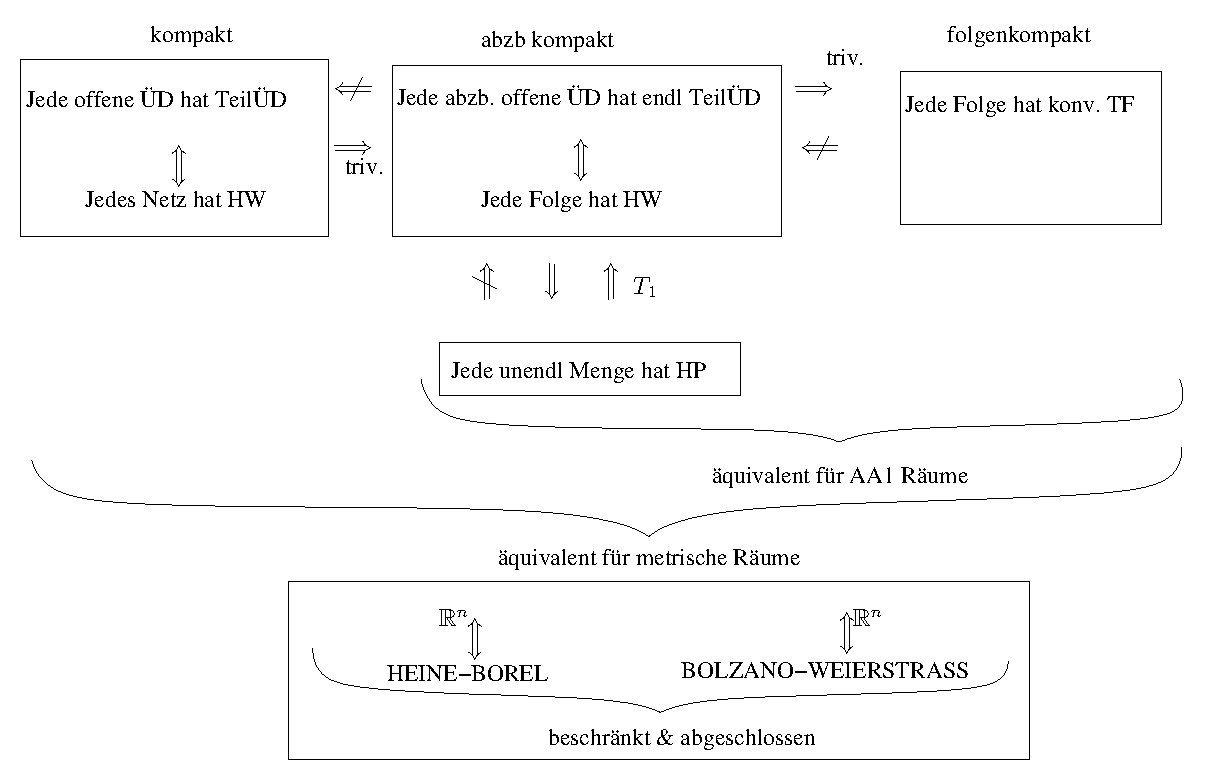
\includegraphics[scale=0.8]{./pic/kompaktheitsbegriffe.eps}
\end{beob}

\begin{definition}\label{6.16}\index{lokalkompakt}Lokalkompaktheit\\
Sei ($X,\T$) ein topologischer Raum.\\
X hei"st \ul{lokalkompakt}:$\eq\forall x\in X\exists$ Umgebungsbasis aus kompakten Mengen
\end{definition}

\begin{beispiel}\label{6.17}zu Lokalkompaktheit
\begin{enumerate}
\item $\R^n$ Die $\ol{B_\eps(x)}$ sind kompakt und bilden eine Umgebungsbasis von x.
\item Offene Teilmengen G von $\R^n$: wie Beispiel 1 (mit $\eps$ passend klein zu x)
\item Abg. Teilmengen von $\R^n: \ol{B_\eps(x)}\cap A$ ist ebenfalls kompakt.
\item $\Q$ ist nicht lokalkompakt, da jedes $(r-\eps ,r+\eps )\cap\Q (r\in\R ,\eps >0)$ Folgen mit irrationalen Limes - also ohne HW in $\Q$ ! -enth"alt. Da Jede Umgebung von r so ein $(r-\eps ,r+\eps )\cap\Q$ enth"alt, kann sie nicht kompakt sein.
\item der {\sc Hilbert}-Raum $\ell^2$ ist nicht lokalkompakt (kein $\infty$-dimensionaler normierter VR ist es!), da keine der abg. Kugeln $\ol{B_\eps(0)}$ kompakt ist - vgl Diskussion zum Satz von {\sc Heine-Borel}.
\end{enumerate}
\end{beispiel}

\begin{prop}\label{6.18}
Sei $(X,\T$) $\trax_2$-Raum dann gilt:\\
X lokalkompakt$\eq \forall x\in X:\exists $ kompakte Umgebung von x
\beweis{
\item[$(\impl$)] klar, nimm irgendeine der kpt. Umgebungen aus der Umgebungsbasis
\item[($\lpmi$)] Sei K kpt. Umgebung von $x\in X$\\
Wir zeigen die Menge aller kompakten Umgebungen von x bilden eine Umgebungsbasis von x.\\
\ul{Vorbemerkung:} Jede $\T|_K$-Umgebung Z von x ist nach \ref{5.2}(i) von der Gestalt $Z=K\cap Z_0$ mit $Z_0\in \umg{U}{x}^X$, somit auch Umgebung von x in ($X,\T$).\hfill ($\star$)\\
Sei jetzt $U\in\umg{U}{x}\impl K\cap U$ ist Umgebung von x in ($K,\T |_K$); wir schachteln im kompakten $\trax_2$-Raum ($K,\T |_K$) ({\scriptsize $\implmit{\ref{6.13}}$normal $\impl$ regul"ar $\impl \trax_3$}) zuerst W, dann V wie folgt ein:\\
$x\in \stackrel{\mbox{\scriptsize offen in K \ref{3.17}(iii)}}{V}\seq \ol{V}^K\seq \stackrel{\mbox{\scriptsize offen in K \ref{2.7}}}{W}\seq K\cap U$\\
Dann gilt:\\
$\bullet$) $\ol{V}^K$ abg. in K $\implmit{\ref{6.8}(i)} \ol{V}^K$ kompakt\\
$\bullet$) $\ol{V}^K$ ist Umgebung von x in K $\implmit{(\star )}$ in X\\
$\bullet$) $\ol{V}^K\seq U$}
\end{prop}
{\bf Bemerkung:} \ref{6.18}(ii)$\impl$ K abg. in X$\impl \ol{V}^X\seq K\implmit{\ref{5.2}(iii)} \ol{V}^K =\ol{V}^X\cap K =\ol{V}^X$.\\
Wichtige Eigenschaften lokalkompakter R"aume:
\begin{enumerate}[(i)]
\item Jeder lokalkompakte Raum X kann durch hinzuf"ugen eines einzigen(!) neuen Punktes ''$\infty''$ kompakifiziert werden, d.h. $X\cap\{\infty\}$ ist kompakt und die Spurtopologie ist die Ausgangstopologie. Hierzu f"ugen wir zu den in X offenen Mengen noch als neue offene Mengen $(X\setminus K)\cup \{\infty\}$ hinzu wobei K kpt.$\seq X$ {\sc Alexandroff}- oder Einpunktkompaktifizierung\\
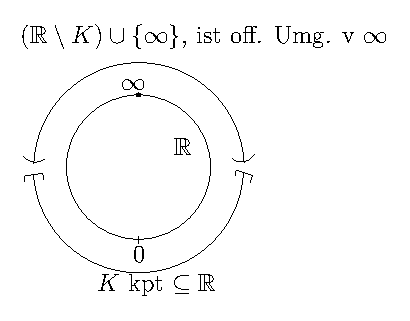
\includegraphics{./pic/alexandroff.eps}\\
\item In lokalkompakten $\trax_2$ R"aumen lassen sich je eine kompakte und eine abgeschlossene Menge ''stetig trennen'' so wie die beiden abgeschlossenen Mengen im {\sc Lemma von Urysohn} (\ref{4.7})
\item Lokalkompakte R"aume sind besonders geeignet f"ur das gleichzeitige betreiben von Ma"stheorie und Topologie - wenn sich die Ma"se mit den Topologien vertragen sollen.
\item Lokalkompakte $\trax_2$-R"aume sind {\sc Baire}'sche R"aume siehe Kapitel VIII.
\end{enumerate}

\section{Connectedness-Zusammenhang}

\begin{definition}\label{7.1}\index{Disjunktion}Disjunktion\\
Sei ($X,\T$) ein topologischer Raum. Eine Disjunktion von X ist ein Paar von offenen, disjunkten Mengen $G_1, G_2$ mit $G_1\cup G_2=X$.
\end{definition}
$G_1$ und $G_2$ k"onnen hier als ''getrennte Teile'' von $X$ aufgefasst werden, ''die von einander topologisch nichts wissen'': $x\in G_1\impl G_1$ ist Umgebung von  x und $G_2$ ist ''weit weg'' von x, da x durch $G_1$ von $G_2$ abgeschirmt wird.\\
Die Mengen sind genau die nichttrivialen ($=\leer , X$) ''\ul{offen-abgeschlossenen}'' Mengen\footnote{engl. ''clopen'' sets - dt. ''abgeschloffen'' ?}\\
Denn: $G_1, G_2$ Disjunktion $\impl X\setminus G_2 =G_1$ ist auch abgeschlossen\\
\hspace*{0.6cm} G offen-abgeschlossen ($\neq \leer ,X ) \impl G, X\setminus G$ ist Disjunktion.\\

\begin{definition}\label{7.2}\index{zusammenhangend@{zusammenh{\"a}ngend}}Zusammenhang\\
Sei ($X,\T$) ein topologischer Raum.\\
X hei"st \ul{zusammenh"angend}$:\eq $ X hat keine Disjunktion.\\
\dots d.h. $\nexists G_1, G_2 \in\T: X=G_1\cup G_2\et G_1\cap G_2 =\leer$\\
Eine Teilmenge A eines topologischen Raumes ($X,\T$) hei"st \ul{zusammenh"angend} :$\eq$ wenn ($A,\T |_A$) zusammenh"angend als topologischer Raum ist.
\end{definition}
Jeder topologische Raum l"asst sich in ''\ul{Zusammenhangskomponenten}''\index{Zusammenhangskomponenten} (maximale zusammenh"angende Teilmengen zerlegen. (ohne Beweis), die bei ''vern"unftigen'' Mengen genau das sind, was man sich erwartet.\\
{\sc achtung} - In allgemeinen F"allen ''Dienst nach Vorschrift''.\\
z.B.: Die Zusammenhangskomponenten von $\Q$ sind genau die Singletons(=Einpunktmengen) $\{ q\}$ mit $q\in\Q$ [w"ahrend $\R$ als Zusammenhangskomponente(n) nur sich selbst besitzt (siehe \ref{7.4}). ]:\\
Enth"alt $A\seq \Q$ zwei verschiedene Punkte $q_1< q_2(\in\Q )$ dann stellen f"ur jede irrationale Zahl $t\in (q_1,q_2)\seq\R$ die Mengen $A\cap (-\infty ,t), A\cap (t,+\infty)$\footnote{diese Mengen hei"sen {\sc Dedekind}'sche Schnitte - mit denen man rechnen kann $\ra$ einen K"orper erh"alt und (oh Wunder) dieser ist als metrischer Raum vollst"andig und wird im Allgemeinen mit $\R$ identifiziert.} bilden eine Disjunktion von A; A ist somit nicht zusammenh"angend.

\begin{satz}\label{7.3}{\sc Stetigkeit und Zusammenhang}\\
Seien ($X,\T_X$), ($Y,\T_Y$) topologische R"aume, $f:X\ramit{stetig} Y$\\
Das stetige Bild zusammenh"angender Mengen ist zusammenh"angend.
\beweis{ Ind. Ann.: Sei $f(X)\seq Y$ nicht zshgd. d.h. $\exists H_1, H_2$ eine Disjunktion - dann ist $\inv{f}(H_1), \inv{f}(H_1)$ eine Disjunktion von X $\wid$ - ein Widerspruch.}
\end{satz}


\begin{satz}\label{7.4}{\sc Die zusammenh"angenden Mengen von $\R$ sind gerade die Intervalle}\\
Sei $A\seq\R$ dann sind die folgende Aussagen "aquivalent:
\begin{enumerate}[(i)]
\item A ist zusammenh"angend
\item A hat die ''Zwischenwerteigenschaft'' (= A ist konvex)\\
$\forall x<y \in A, t\in \R$ und $x<t<y\impl t\in A$.
\item A ist ein Intervall.
\end{enumerate}
\beweis{\item[$(i)\impl (ii)$] Indirekt: Ist (ii) verletzt, dann $\exists x,y\in A, t\in \R$ mit $x<t<y$ und $t\notin A$; dann ist $(-\infty ,t)\cap A, (t,+\infty )\cap A$ eine Disjunktion von A $\wid$ - ein Widerspruch.
\item[$(ii)\impl (i)$] Indirekt:Sei $A_1, A_2$ Disjunktion von A$:\eq\exists G_1, G_2 \mbox{\scriptsize offen}:A_1 =A\cap G_1$ und  $A_2 =A\cap G_2$ und $A=\underbrace{(A\cap G_1)}_{\mbox{\scriptsize offen in A}}\cup \underbrace{(A\cap G_2)}_{\mbox{\scriptsize offen in A}}$, $\underbrace{(A\cap G_1)}_{\neq\leer}\cap \underbrace{(A\cap G_2)}_{\neq\leer }=\leer$\\
W"ahle $u_1\in (A\cap G_1), u_2\in (A\cap G_2)$; oBdA. $u_1<u_2$; nach (ii) ist $[u_1, u_2]\seq A$ und $[u_1,u_2]\cap G_1, [u_1,u_2]\cap G_2$ eine Disjunktion von $[u_1,u_2] \wid$ - ein Widerspruch: Sei $z:=\sup ([u_1,u_2]\cap G_1) \in [u_1,u_2]$. Dann muss $z$ in $G_1$ oder in $G_2$ liegen, beides ist aber unm"oglich; da $G_1, G_2$ offen.
\begin{itemize}
\item $z\in G_1(\impl z<u_2)\impl$ ein ganzes Intervall $[z,z+\delta ) (\delta >0)$ geh"ort also ebenfalls noch zu $[u_1, u_2]\cap G_1 \wid$ ein Widerspruch zu $z=\sup ([u_1,u_2]\cap G_1)$
\item $z\in G_2 (\impl z>u_1)\impl$ ein Intervall $(z-\eta ,z ] (\eta >0)$ geh"ort ebenfalls noch zu $[u_1,u_2]\cap G_2 \wid$- ein Widerspruch zu $z=\sup ([u_1,u_2]\cap G_1)$.
\end{itemize}
\item[$(ii)\impl (iii)$] $A=\leer $: ok; f"ur $A\neq\leer$ setzen wir:\\
$a:=\inf (A) \in \R\cup\{ -\infty\}\quad (\impl a\leq t\in A)$\\
$b:=\inf (A) \in \R\cup\{ +\infty\}\quad (\impl A\ni t\leq b)$\\
F"ur $a<z<b$ w"ahlen wir  $u\in A\cap (a,z)$, $v\in A\cap (z,b)$\\
Dann ist $u<z<v$ und nach (ii) somit $z\in A$\\
$\impl (a,b)\seq A\seq [a,b] (\seq \R\cup\{ -\infty ,+\infty\} )$
\item[$(iii)\impl (ii)$] $A=\leer$ oder $A=\{ a\}:$ ok; sei nun $a<b$ und $A=[a,b];$ f"ur $x,y\in A$ und $x<z<y$ gilt nun $a\leq x<z<y\leq b\impl z\in [a,b]=A$. Die F"alle $A= (a,b], [a,b), (a,b); (-\infty ,b), (-\infty ,b], (a,+\infty ), [a, +\infty )$ gehen analog.}
\end{satz}

\begin{kor}\label{7.5} zu \ref{7.3} und \ref{7.4} ({\sc Zwischenwertsatz})\\
Sei $(X,\T$) topologischer, zusammenh"angender Raum und $f:X\ramit{\mbox{\scriptsize stetig}}\R$\\
F"ur $x_1, x_2\in X$ und $f(x_1)<t<f(x_2)$ existiert ein $x\in X$ mit $f(x) = t$.
\beweis{Nach \ref{7.3} ist $f(X)$ zusammenh"angende Teilmenge von $\R$, hat also nach \ref{7.4} $(i)\impl (ii)$ die Zwischenwerteigenschaft.\\
F"ur den Spezialfall, dass X ein Teilintervall von $\R$ ist (\ref{7.4} $(iii)\impl (i)$), liefert \ref{7.5} den {\sc Zwischenwertsatz} der reellen Analysis.}
\end{kor}

\begin{definition}\label{7.6}\index{zusammenhangend@{zusammenh{\"a}ngend}!bogenweise}
Sei ($X,\T$) topologischer Raum.\\
X hei"st \ul{bogenweise zshgd}$:\eq\forall x,y\in X\hspace*{-1.4cm}\underbrace{\exists c:[0,1]\ramit{stetig} X}_{\mbox{\scriptsize stetiger Pfad/Kurve, der x mit y verbindet}}$\hspace*{-1.4cm} mit $c(0)=x, c(1)=y$
\end{definition}

\begin{prop}\label{7.7}{bogenweise zusammenh"angend $\impl$ zusammenh"angend}\\
Sei ($X,\T$) ein topologischer Raum, X bogenweise zusammenh"angend, dann ist X auch zusammenh"angend.
\beweis{Indirekt angenommen: Sei $G_1, G_2$ eine Disjunktion von X, dann w"ahlten wir $x\in G_1$, $y\in G_2$ und verbinden x und y mit dem stetigen Pfad c. Dann liefert $\inv{c}(G_1),\inv{c}(G_2)$ eine Disjunktion von $[0,1] \wid$ - ein Widerspruch nach \ref{7.4} $(iii)\impl (i)$}
\end{prop}
Die Menge $\{ 0\}\times [-1,+1]\cup\{ (x,\sin(\frac{20}{x}) )|x\in (0,1]\}\seq \R^2$ mit der Spurtopologie, ist zusammenh"angend, aber nicht bogenweise zusammenh"angend ([CR] p.152-153)\\
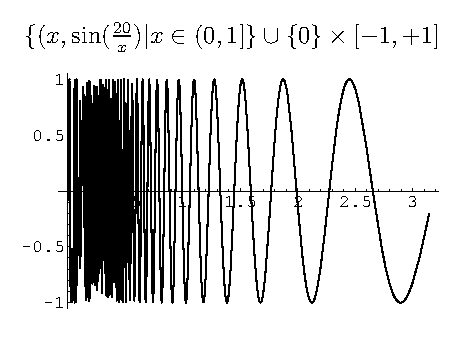
\includegraphics[scale=0.82]{./pic/zshg.eps}\\
(P,Q k"onnen nicht durch einen stetigen Pfad in X verbunden werden.)\\
Allerdings gilt: Ist X zusammenh"angend und besitzt f"ur jeden $x\in X$ eine bogenweise zusammenh"angende Umgebung, dann ist X bogenweise zusammenh"angend ([CR]p.154). Damit ist jede \ul{offene} zusammenh"angende Teilmenge G (ein ''\ul{\bf G}ebiet[!]) des $\R^n$ auch bogenweise zusammenh"angend.

\section{Spezielle Resultate "uber metrische R"aume}
Im ganzen Kapitel sei $(X, d$) metrischer Raum und $\T_d$ die von $d$ erzeugte Topologie auf X (die ''metrische Topologie'').
\begin{itemize}
\item Kompaktheit (\ref{6.15}) 
\item Normalit"at ($\trax_4 +\trax_1$)
\item Vollst"andigkeit, Vervollst"andigung
\item Fixpunktsatz von {\sc Banach}\item Satz von {\sc Baire}
\end{itemize}
\subsection{Kompaktheit}
Siehe Kapitel VI
\subsection{Normalit"at}
F"ur $\leer \neq C\seq X$ und $x\in X$ definieren wir den \ul{Abstand von x zu C}\index{Abstand von einer Menge} durch:
$$d(x,C):=\inf\{d(x,y)|y\in C\}$$
Dann gilt:
\begin{itemize}
\item $d(x,C)=0\eq x\in\ol{C}$ ($\dots x_n\ra x, x_n\in C, d(x,x_n)\ra d(x,C)\dots$)\\
\includegraphics{./pic/d(xC).eps}
\item $x\mapsto d(x,C)$ ist stetig, denn es gilt $|d(x,C) -d(y,C)|\leq d(x,y):\\
z_n\in C, d(x,z_n)\ra d(x,C): d(x,C)\leq d(x,z_n)\leq d(x,y)+d(y,z_n)\ra d(x,y)+d(z,C)$\\
analog $d(y,C)\leq d(x,y)+d(y,C)$.
\end{itemize}

\begin{satz}\label{8.1}{\sc Jeder metrische Raum ist Normal}{ mit der metrischen Topologie}
\beweis{\item[$\bullet$] metrisch $\implmit{\ref{3.15}(i)} \trax_2\impl \trax_1$
\item[$\bullet$] A,B (disj.\& abg.)$\seq X; dann ist :$
$$f(x):=\frac{d(x,A)}{d(x,A)+d(x,B)} (x\in X)$$
stetig, $f:X\ra [0,1], f|_A=0, f|_B=1$ (wie im {\sc Lemma von Urysohn}\ref{4.7}$\impl \trax_4$}
\end{satz}

\subsection{Vollst"andigkeit \& Vervollst"andigung}
\begin{definition}\label{8.2} Cauchy-Folge\index{Cauchyfolge@{\sc Cauchy}-Folge} \\
Sei $(x_n)_{n\in\N}$ eine Folge in X, dann hei"st:\\
$(x_n)_{n\in\N}$ \ul{Cauchy-Folge}$:\eq \forall\eps >0 \exists N\in\N :\forall m>n\geq N: d(x_m,x_n)<\eps$
\end{definition}
\ul{\bf Bemerkung:} $(x_n\ra x)\impl (x_n)_{n\in\N}$ Cauchy-Folge, denn $d(x_n,x_m)\leq d(x_n, x)+d(x,x_m)$.

\begin{definition}\label{8.3} gleichm"a"sig stetig \index{Stetigkeit!gleichmassige@gleichm{\"a}{\ss}ige}\\
Seien $(X,d_X), (Y,d_Y)$ metrische R"aume, $f:X\ra Y$\\
f \ul{gleichm"a"sig stetig}$:\eq \forall\eps >0 \exists\delta >0\forall x,y\in X: d_X(x,y)<\delta :d_Y(f(x),f(y))<\eps$
\end{definition}
Gleichm"a"sig stetige Abbildungen bilden Cauchy-Folgen auf Cauchy-Folgen ab.
\begin{definition}\label{8.4} Vollst"andigkeit \index{Vollstandigkeit@Vollst{\"a}ndigkeit}
Sei (X, d) metrischer Raum\\
(X,d) \ul{vollst"andig}$:\eq (x_n)_{n\in\N}$ Cauchy-Folge $\exists x\in X: x_n\ra x$.
\end{definition}

\begin{beispiel}\label{8.5} zur Vollst"andigkeit:
\begin{enumerate}
\item $(E,\norm{\_})$ normierter Vektorraum, $d(x,y):=\norm{x-y}\\
(E,\norm{\_})$hei"st \ul{{\sc Banach}-Raum}\index{Banachraum@{\sc Banach}-Raum}$:\eq (E,\norm{\_})$ vollst"andig.
\item $(E,\innprod{\_}{\_})$ Raum mit inneren Produkt, $d(x,y):=\sqrt{\innprod{x-y}{x-y}}=\sqrt{\norm{x-y}_2}$:\\
$(E,\innprod{\_}{\_})$ hei"st \ul{{\sc Hilbert}-Raum}\index{Hilbertraum@{\sc Hilbert}-Raum}$:\eq (E,d)$ vollst"andig.
\end{enumerate}
\end{beispiel}

\begin{beob}\label{8.6} (leichte Beweise)
\begin{enumerate}[(i)]
\item $(X,\T_d)$ metrischer kompakt Raum$\impl (X, d)$ vollst"andig.
\item Sei $(X,d)$ vollst"andig, $A\seq X$\\
A abgeschlossen $\eq$ A vollst"andig (bez"uglich $d|_{A\times A}$)
\end{enumerate}
\end{beob}
Beispielsweise ist $\mathcal{C} ([a,b])$ abgeschlossen im {\sc Banach}-Raum $(\mathcal{B}([a,b],\norm{\_}_\infty )$ der beschr"ankten Funktionen (Analysis-VO!), daher ist auch ($\mathcal{C}([a,b]),\norm{\_}_\infty$) der Raum der stetigen Funktionen auf Kompaktum ein {\sc Banach}-Raum.\vspace*{0.3cm}\\
Jedem nicht-vollst"andigen metrischen Raum kann man die ''fehlenden'' Limiten von Cauchy-Folgen derart dazugeben, sodass ein vollst"andiger metrischer Raum entstehen.

\begin{definition}\label{8.7} Vervollst"andigung\index{Vervollstandigung@Vervollst{\"a}ndigung}
Sei $(X,d)$ ein metrischer Raum, dann hei"st ein vollst"andiger, metrischer Raum $((\widetilde{X},\widetilde{d}),\iota$) zusammen mit einer injektiven Abbildung $\iota :X\inj\widetilde{X}$ \ul{Vervollst"andigung} wenn gilt:
\begin{enumerate}[(i)]
\item $\widetilde{d}(\iota (x),\iota (y))= d(x,y)\quad (x,y\in X)$\hfill d.h. $\iota$ ist Isometrie
\item $\ol{\iota (X)}=\widetilde{X}$\hfill d.h. $\iota (X)$ ist dicht in $\widetilde{X}$
\end{enumerate}
Identifizieren wir X mit $\iota (X)$ $(x\leftrightarrow \iota (x), x\in X)$, dann erhalten (i) und (ii) die Gestalt:
\begin{enumerate}[(i)']
\item $\widetilde{d}|_{X\times X} =d$\hfill {\scriptsize ($\widetilde{d}$ setzt d fest)}
\item $\ol{X} = \widetilde{X}$\hfill {\scriptsize ($X$ liegt dicht in $\widetilde{X}$)}
\end{enumerate}
\includegraphics{./pic/vervollstandigung.eps}
\end{definition}
\begin{satz}\label{8.8}{\sc "Uber Existenz und Eindeutigkeit von Vervollst"andigungen}
\begin{enumerate}[(i)]
\item Zu jedem metrischen Raum $(X,d)$ existiert (mindestens) eine Vervollst"andigung.
\item Je zwei Vervollst"andigungen sind isometrisch-isomorph($\leadsto $''die'' Vervollst"andigung:\\
$\xymatrix@R=0.1cm{
&\widetilde{X}\ar@{<->}[dd]^{\mbox{\scriptsize bij}}\\
X\ar@{}[ur]|\seq \ar@{}[dr]|\seq \\
&\widetilde{\widetilde{X}}
}$
\item Jede gleichm"a"sig stetige Abbildung $f$ von $(X,d_X)$ in einen vollst. metr. Raum $(Y,d_Y)$ l"asst sich eindeutig zu einer gleichm"a"sig stet. Abbildung\\
$\widetilde{f}:\widetilde{X}\ra Y$ fortsetzen:
$\xymatrix{X\ar@{^{(}->}[r]^\iota \ar[dr]_f&\widetilde{X}\ar@{-->}[d]^{\exists !\widetilde{f}}\\
&Y}$
$\widetilde{f}\circ \iota =f; \widetilde{f}(\hspace*{-0.6cm}\stackrel{\stackrel{\lim x_n, x_n\in X}{\lightning}}{\widetilde{x}}\hspace*{-0.6cm})=\lim_{n\in\N}\hspace*{-0.2cm}\underbrace{f(x_n)}_{\mbox{\scriptsize ist C.F. in Y}}$
\end{enumerate}
\beweis{
\item[ad (i)] \framebox{Entweder} $\widetilde{X}$ als Menge aller Cauchy-Folge in X konstruieren, wobei $(x_n)_{n\in\N}$ und $(y_n)_{n\in\N}$ identifiziert werden, wenn $d(x_n,y_n)\ra 0$ gilt:\\
$$\widetilde{X}:=\{(x_n)_{n\in\N}|(x_n)\mbox{ist Cauchy-Folge in X}\}/_\sim \mbox{ mit } (x_n)_{n\in\N}\sim (y_n)_{n\in\N}:\eq d(x_n,y_n)\ra 0$$
$$\iota (x):=[(x,x,x,\dots )]$$
[Funktioniert als ''Kaltstart'' f"ur die Vervollst"andigung von $\Q$ zu $\widetilde{\Q}=\R$.]\\
\framebox{Oder} [Wir setzen $\R$ als vollst"andig voraus und \dots ]\\
Betten X isometrisch in den vollst"andigen, metrischen Raum $\mathcal{C}_b (X,\R)$ der beschr"ankten stetigen Funktionen von $X$ nach $\R$, mit der Metrik $d(f,g):=\norm{f-g}_\infty$, $\norm{h}_\infty :=\sup_{x\in X}|h(x)|$ ein: Fixiere $a\in X$ (bel.) und definiere: $g:X\ra \mathcal{C}_b (X,\R)$ durch $g:x\mapsto (g_x:y\mapsto d(x,y) -d(a,y))$ und setze $\widetilde{X} =\ol{g(x)}, \iota =g$ (siehe [CR] p.55-56).
\item[ad (iii)] Beweisidee: F"ur $\widetilde{x}=\lim_{n\in\N}\hspace*{-0.7cm}\blitzmit{x_n}{\mbox{\scriptsize Cauchy-Folge}\impl}\hspace*{-0.7cm}, x_n\in X$ setze $\widetilde{f}(\widetilde{x}):=\lim_{n\in\N}\overbrace{f(x_n)}^{\impl \mbox{C.F.}}$
\item[ad (ii)] $\xymatrix{
	X
		\ar@{^{(}->}[rr]^{\widetilde{\iota}}
		\ar@<-0.1cm>@{^{(}->}[drr]^{\widetilde{\widetilde{\iota}}}
 &&{\widetilde{X}\mbox{\scriptsize(Vervollst.)}}
		 \ar [d]^{\exists !\varphi}\\
&& \widetilde{\widetilde{X}}
}$
$\xymatrix{
	X
		\ar@{^{(}->}[rr]^{\widetilde{\iota}}
		\ar@<-0.1cm>@{^{(}->}[drr]^{\widetilde{\widetilde{\iota}}}
 && {\widetilde{X}
		\mbox{\scriptsize(Vervollst.)}}\\
&& \widetilde{\widetilde{X}}\ar [u] _{\exists !\psi}
}$\\
Zeige dann (ebenfalls mit Dreiecksdiagrammen: $\psi\circ\varphi =id_{\widetilde{X}}$, $\varphi\circ\psi =id_{\widetilde{\widetilde{X}}}$;\\
$\varphi$ und $\psi$ sind inverse Isometrien.}
\end{satz}
\subsection{Fixpunktsatz von {\sc Banach}}
\begin{satz}\label{8.9}{\sc Fixpunktsatz von Banach}\\
Sei ($X,d$) ein vollst"andiger metrischer Raum und $T:X\ra X$ eine Kontraktionsabbildung, d.h. $d(T(x),T(y))\leq Kd(x,y)$ f"ur ein$K\in(0,1)$ und $x,y\in X$;\\
Dann besitzt $T$ einen Fixpunkt (d.h. $Tx=x$) - dieser ist eindeutig und gegeben durch: $z=\lim_{n\in\N}T^nx$ f"ur jeden beliebigen Startpunkt.
\beweis{Sei $x\in X$(bel.) und $T^1x=Tx, T^n:=T(T^{n-1}x)$.  Dann gilt:\\
$d(T^{n+1}x,T^nx)\leq K^nd(Tx,x)$ und f"ur $m>n$:\\
$d(T^mx,T^nx)\hspace*{-0.8cm}\blitzmit{\leq}{\triangle -Ungleichung} \hspace*{-0.8cm}d(T^mx,T^{m-1})+d(T^{m-1}x,T^{m-2}x)+\dots +d(T^{n+1}x,T^nx)\leq\\
\hspace*{2.3cm}\leq (K^{m-1}+K^{m-2}+\dots +K^n)d(Tx,x)=\\
\hspace*{2.3cm}=\frac{K^n}{1-K}d(Tx,x)$\\
Wegen $K^n\ra 0$ f"ur $n\ra\infty$ ist $(T^nx)_{n\in\N}$ eine C.F., sei $z=\lim_{n\in\N}T^nx$.\\
Dann gilt (T ist stetig, sogar {\sc Lipschitz}-stetig):
$$Tz=T(\lim_{n\in\N}T^nx) = \lim_{n\in\N}T(T^nx)=\lim_{n\in\N}T^{n+1}x=z$$
Sei $u\neq z$ ein zweiter Fixpunkt, also  $Tu=u$, dann folgt:\\
$0<d(z,u)=d(Tz,Tu)\leq Kd(z,u) \wid$ ein Widerspruch, da $K<1$, also ist $d(z,u)=0\eqmit{D0} z=u$}
\end{satz}

\subsection{Satz von {\sc Baire}}
\begin{definition}\label{8.10}\index{nirgends dicht}\index{mager}
Sei $(X,\T)$ topologischer Raum, $A\seq X$ dann hei"st:\\
A \ul{nirgends dicht}$:\eq \inn{(\ol{A} )}=\leer$\\
A \ul{mager}$:\eq \exists A_1, A_2\dots ;$ all nirgends dicht und $A=\bigcup_{i=1}^\infty A_i$\\
$[$Genaugenommen: ''nirgends dicht \ul{in X}'', und ''mager \ul{in X}'', $\inn{(\ol{A}^X)}]$
\end{definition}
Nirgends dichte (n.d.) Mengen sind ''kleine, d"unne Mengen'' im topologischen Sinne: Ihre Abschl"usse enthalten keine nichtleeren, offenen Mengen und keine Umgebungen.\\
Da endliche Vereinigung von n.d. Mengen wieder nirgends dicht sind (siehe \ref{8.12}(iii)), sind magere Mengen in gewissem Sinn der ''n"achstgr"o"sere'' Typ von Mengen. Sie hei"sen daher manchmal auch ''Mengen 1.Kategorie''; eine ''Menge 2. Kategorie'' ist dann eine nichtmagere Menge.
\begin{beispiel}\label{8.11} zu nirgends dichten und mageren Mengen
\begin{enumerate}
\item Jedes $\{ x\}$ ist nirgends dicht in $\R$; jede Gerade in $\R^2$ und Ebene in $\R^3$.
\item $\Q =\bigcup_{q\in\Q}\{ q\}$ ist mager in $\R$, eine abzb. Vereinigung von Geraden im $\R^2$ ist mager usw.
\end{enumerate}
\end{beispiel}

\begin{beob}\label{8.12} zu nirgends dichten und mageren Mengen
\begin{enumerate}[(i)]
\item A (n.d.) und $B\seq A \impl B$ ist nirgends dicht, denn $B\seq A\impl\inn{(\ol{B})}\seq\inn{(\ol{A})}$
\item A mager und $B\seq A\impl B$ mager denn $B=B\cap A=B\cap (\bigcup_{i=1}^\infty A_i)= \bigcup_{i=1}^\infty \underbrace{(B\cap A_i)}_{\mbox{n.d.}}$
\item $A, B$ n.d. $\impl A\cup B$ n.d. denn sei:\\
$G${\scriptsize (offen)}$\seq\ol{A\cup B}\gleichmit{\ref{2.35}(iv)} \ol{A}\cup\ol{B}$\\
$G\setminus\ol{A}${\scriptsize (offen)}$\seq \ol{B}\implmit{B n.d.} G\setminus\ol{A} =\leer\impl G\seq \ol{A}\implmit{A n.d.} G=\leer$
\item A n.d. $\eq \inn{(\ol{A})}$\\
\hspace*{1.3cm}$\eq $ keine nichtleere offene Menge ''passt'' in $\ol{A}$ ''rein''\\
\hspace*{1.3cm}$\eq$ jede nichtleere offene Menge ''steht'' "uber $\ol{A}$ ''raus''\\
\hspace*{1.3cm}$\eq$ jede nichtleere offene Menge enth"alt $\ext{A}$-Punkte\\
\hspace*{1.3cm}$\eq \ext{A}$ ist dicht.
\end{enumerate}
\end{beob}

\begin{satz}\label{8.13}{\sc Satz von Baire}\\
In einem vollst. metrischen Raum $(X,d)$ ist das Innere jeder mageren Menge leer.
\beweis{Sei A mager$:\eq A=\bigcup_{i=1}^\infty A_i, A_i$ n.d.\\
Sei $x_0\in X, r_0 >0$(bel.) : Wir zeigen A kann $B_{r_0}(x_0)$ {\sc nicht} enthalten.\\
Mittels Induktion definieren wir eine Folge von B"allen:\\
$B_1\supseteq B_2\supseteq B_3\supseteq\dots$,  $B_n:=B_{r_n}(x_n), r_n<\durch{n}$, so:\\
$B_{n-1}$ gew"ahlt$\implmit{A_n n.d.}\exists x_n\in B_{n-1}\setminus\ol{A_n}=B_{n-1}\cap(\ol{A_n})^c$ ist offen!\\
$\impl \exists r_n(<\durch{n}): x_n\in B_{r_n}(x_n)\seq \ol{B_{r_n}(x_n)}\seq B_{n-1}\setminus\ol{A_n}$\\
$\bullet )$ $(x_n)_{n\in\N}$ ist Cauchy-Folge, da f"ur $m>n: x_m\in B_n\impl d(x_n,x_m)<r_n$\\
$\bullet )$ X vollst"andig$\impl \exists X\in x\lim_{n\in\N}x_n$\\
$\bullet )$ $x_m\in\ol{B_n}$ f"ur $m>n \impl x=\lim_{m\in\N}x_m\in\ol{B_n}\forall n\in\N$\\
\hspace*{0.3cm} $\impl x\in \bigcap_{n=1}^\infty \ol{B_n}\seq \bigcap_{n=1}^\infty (B_n\cap \ol{A_n}^c) =\bigcap_{n=1}^\infty B_n\cap (\bigcup_{n=1}^\infty A_n)^c \seq B_0\setminus A$\\
A enth"alt also keine offene Kugel $B_0$, somit ist $\inn{A}=\leer$}
\end{satz}
\ul{\bf Bemerkung:}
\begin{enumerate}[(i)]
\item Insbesondere kann ein vollst"andiger metrischer Raum nicht selbst mager (in sich) sein.
\item Ist $(X,d)$ nicht vollst"andig, dann kann X sehr wohl mager (in sich) sein, z.B. $\Q =\bigcup_{q\in\Q} q$.
\end{enumerate}
F"ur Anwendungen des Satzes von {\sc Baire} siehe [CR] p.63-65 oder auch\\
\verb*|http://www.mat.univie.ac.at/~cap/files/Topologie.pdf|\\
Oft findet sich statt ''Das Innere magerer Mengen ist leer.'' auch eine der folgenden "aquivalenten Bedingungen; solche R"aume hei"sen {\sc Baire}'sche R"aume. Nach \ref{8.13} ist also jeder vollst"andige metrische Raum {\sc Baire}'sch; andererseits auch jeder lokalkompakte (nach \ref{6.18} auch jeder kompakte) {\sc Hausdorff}-Raum {\sc Baire}'sch - siehe [CR] p.128 .

\begin{prop}\label{8.14} F"ur einen topologischen Raum $(X,\T$) sind die folgenden Eigenschaften "aquivalent (und charakterisieren {\sc Baire}'sche R"aume):
\begin{enumerate}[(i)]
\item A mager $\impl \inn{A}=\leer$
\item A mager $\impl A^c$ dicht
\item G nichtleer, offen $\impl$ G nicht mager
\item $G_1, G_2,\dots $ alle offen und dicht $\impl \bigcap_{n=1}^\infty G_n$ dicht
\end{enumerate}
\beweis{
\item[(i)$\eq$(ii)]$\inn{A} =\ext{A^c} =\leer \eq \ol{(A^c)}=X\eq A^c$ ist dicht\hfill $(\star)$
\item[(i)$\impl$(iii)] Indirekt angenommen:G mager $\implmit{(i)} G=\inn{G} =\leer \wid$ ein Widerspruch.
\item[(iii)$\impl$(i)] Indirekt angenommen $\inn{A}\neq \leer\impl \inn{A}$ nichtleer, offen, mager ($\seq A$-\ref{8.12}(ii))$\wid$ ein Widerspruch.
\item[(i)$\impl$(iv)] $G_n$ offen, dicht $\implmit{(\star )} G_n^c$ (abg.)$\et \inn{(G_n^c)}=\leer \impl G_n^c$ n.d.\\
\hspace*{3cm} $\impl \bigcup_{n\in\N}G_n^c$ mager $\implmit{(i)} \inn{(\bigcup_{n\in\N}G_n^c)}=\leer$\\
\hspace*{3cm} $\implmit{(\star )} (\bigcup_{n\in\N}G_n^c)^c=\bigcap_{n\in\N} G_n$ dicht
\item[(iv)$\impl$(i)] Sei $A=\bigcup_{n\in\N}A_n, A_n$ n.d.; $G_n:=(\ol{A})^c\implmit{(\star )} G_n$ dicht\\
\hspace*{3cm} $\bigcap_{n\in\N} G_n$ dicht $\implmit{(\star )}(\bigcap_{n\in\N}G_n)^{c\circ}=\leer$\\
\hspace*{3cm} $\inn{(\bigcup_{n\in\N}G_n^c)}=\inn{(\bigcup_{n\in\N}\ol{A_n})}=\leer\impl\inn{A}=\inn{(\bigcup_{n\in\N}A_n)}=\leer$}
\end{prop}
\newpage
\thispagestyle{empty}
\printglossary
\newpage
\printindex
\end{document}
